% !Mode:: "TeX:UTF-8"

\chapter{分层光网络下的并行路由优化算法研究}
\section{引言}
在EON架构中,存在细粒度的带宽间隙(比如,12.5GHZ),他比WDM 网络所遵循的ITU标准的50GHZ或者100GHZ 的带宽粒度要小很多,而且,这些带宽间隙可以根据需要被组合在一起以提供更宽的通道。为了提高带宽利用率,在EON中存在混合速率,每个速率的业务需要不同数量的频谱间隙数量。理论上,EON能够灵活地提供各种速率,但是在实际中,EON却可能只含有很少的速率种类,这主要是因为:第一,随着频谱的增加,频谱碎片和管理复杂度将显著增加。第二,实际的EON从较低的线路费率升级到更高的线路费率,并存大量速率的情况已经很少见了。

为了在EON网络中加入业务,控制平面必须在网络中找到一条路径,同时,还需要在此路径上的链路上分配足够的频谱带宽,来创建一个合适的端到端光路连接,这被称为路由和频谱分配(RSA)问题,RSA问题可以进一步分为静态RSA问题和动态RSA问题。静态的RSA问题出现在网络规划阶段,其中流量需求是已知的,这样可以离线计算出最优或者接近最优的RSA解,动态RSA问题是指在实时业务情况下光通路的路由选择和波长分配的优化问题,在动态RSA问题中,业务随机的到达和离开光网络,而且当业务到达网络时,控制平面需要在短时间内找到RSA解来安排业务。动态RSA问题比静态RSA问题更具有挑战性,因为业务需求随机到达和离开,网络状况随时发生变化,而且要求控制平面反应实时。

本章考虑在EON中解决动态场景下的业务量工程问题,我们采用分层图模型将频谱分配问题简化为路由选择问题,设计出基于分层图模型的频谱分配与业务量工程算法(TESAA,traffic engineering and sptrum allocate algrithm),在进行频谱分配的同时优化路由代价。我们针对算法TESAA进行并行加速设计,在带权图和无权图两种情况下对TESAA进行GPU并行加速,实验发现,基于GPU的并行的PTESAA(parallel TESAA)算法对串行算法STESAA(serial TESAA)的加速比可达到5倍。我们将PTESAA与基于分层图模型的贪心算法比较,发现PTEAA在短时间内能够大大地优化路由代价,并且由于路由代价减小,占用网络资源较少,最终使得网络阻塞率降低。
\section{问题描述}
\subsection{EON中动态RSA问题}
当业务到达网络时,SDN控制层需要找到可行的路径,并且为路径分配合适的频谱资源。由于EON的物理限制,RSA问题的解需要满足以下限制:

第一,传输距离限制:光信号的传输质量会随着传输距离的增加而下降,为了在目的点顺利恢复光信号,光链路的传输距离需要小于一个阈值$W_{max}$, 为了简化设计,本文假设每一条链路的长度相同,都是一个单位,那么传输路径的跳数需要小于阈值$D_{max}$。

第二,频谱连续性限制:每条光连接的频谱从它的源节点到它的目的节点 ,在所经过的链路上保持不变。

第三,频谱不重叠限制:同一光纤链路中的频谱不能分配给不同的光路。

第四,频谱邻近限制:频谱邻近约束保证分配给一个光路径的频谱必须是一个连续的部分。
\subsection{分层网络模型}
论文 \citing{ELAYER}中提出一种分层图模型来解决WDM网络中的路由和波长分配问题,分层图模型将路由选择和波长分配问题统一到一起来,使得RWA问题变得简化,这种分层图模型也可以很容易推广到EON的RSA问题中。

我们使用有向图$N(V,E)$表示物理网络拓扑,其中$V=\{v_1,v_2,...,v_N\}$表示节点集合,$E=\{e_1,e_2,e_3,...,e_M\}$表示边集合,$e_k=(i_k,j_k)$表示边的头节点为$v_{i_k}$,边的尾节点为$v_{j_k}$。假设所有光链路具有相同的频谱范围$W=(F_{start},F_{end})$, 其中$F_{end}-F_{start}=C$。EON所支持的速率集合为$R$, 比如,$R={40Gb/s,100Gb/s,400Gb/s}$, 每一种速率$r\in R$需要一个特定的频谱宽度$b_r GHz$。一个源节点为$s$,目的节点为$t$,速率为$r Gb/s$的业务被表示为$TD(s,t,r)$。

下面我们讨论分层图的产生过程,假设第一个速率的为$r$的业务$TD_r(s,t)$到达网络,我们从可用的频谱切割出一块频谱大小为$b_r$ 的连续带宽分配给速率为$r$ 的业务,假设这块频谱的起始频率为$fs_{( r,1 )}$,终止频谱为$fe_{( r,1 )}$,那么$fe_{( (r,1) )}-fs_{( (r,1) )}=b_r$,我们把所有物理链路上频谱范围$( fs_{( (r,1) )},fe_{( (r,1) )} )$,从所有链路上切割下来,把切割下来的部分组成一个新的虚拟网络$N^{( r,1) )} ( V^{( (r,1) )},E^{( (r,1) )}) )$,在这个新的网络中每条链路的频谱范围都是$(fs_{( (r,1) )},fe_{( (r,1) )})$,这样切割下来之后,原来的物理网络的频谱范围更新为$( F_{start}+b_r,F_{end} )$。

如果在这个复制出来的图上为业务求一条最短路径$p$,那么容易知道路径$p$一定满足约束2,3,4, 这样问题被简化为单纯的路由问题。要注意的是,这个虚拟图上频谱不能再分配给其他速率为$r'$ 的业务$TD_{r'}(s',t')$, 即使$b_r'<b_r$,这是因为这样会产生大量的频谱碎片,使得频谱利用率下降,并且这样会使得问题变得更加复杂化,所以这些分割出来给速率$r$的频谱,将继续被分配给速率为$r$ 的业务。当下一个速率为$r$的业务$TD_r (s'',t'')$ 到达网络后,他首先在图$N^{( r,1) )} ( V^{( (r,1) )},E^{( (r,1) )}) )$中寻找路径,如果找到合适的路径则加入网络并且更新路径链路的可用频谱为0;反之,如果他在图$N^{( r,1) )} ( V^{( (r,1) )},E^{( (r,1) )}) )$中没有找到合适的路径,那么算法会重新去”切割“物理拓扑得到虚拟网络$N^{( r,2) )} ( V^{( (r,2) )},E^{( (r,2) )}) )$,这样随着大量业务的动态的到达和离去,会产生大量的分层图,频谱资源已经大量地分布在各个虚拟图中,我们把这些虚拟图叫做分层图(layered Graph),现在RSA问题转化为在分层图中求解路由的问题,问题被简化。
下图 \ref{layer}表示分层图示意,原图被切割成一个分层图集集合$L$,$L_i \in L$表示速率$i$的分层图集,如图所示,速率$k$的一共有$|L_k|$ 个图副本,每个子分层图占用频谱$(fs_{( (r,1) )},fe_{( (r,1) )})$,图 \ref{layer}中,点$v_i^{( (r,l) )}$表示速率$r$ 的第$l$ 层图上的第$i$ 号点。
\begin{figure*}
\setlength{\belowcaptionskip}{-0.5cm}
\begin{center}
{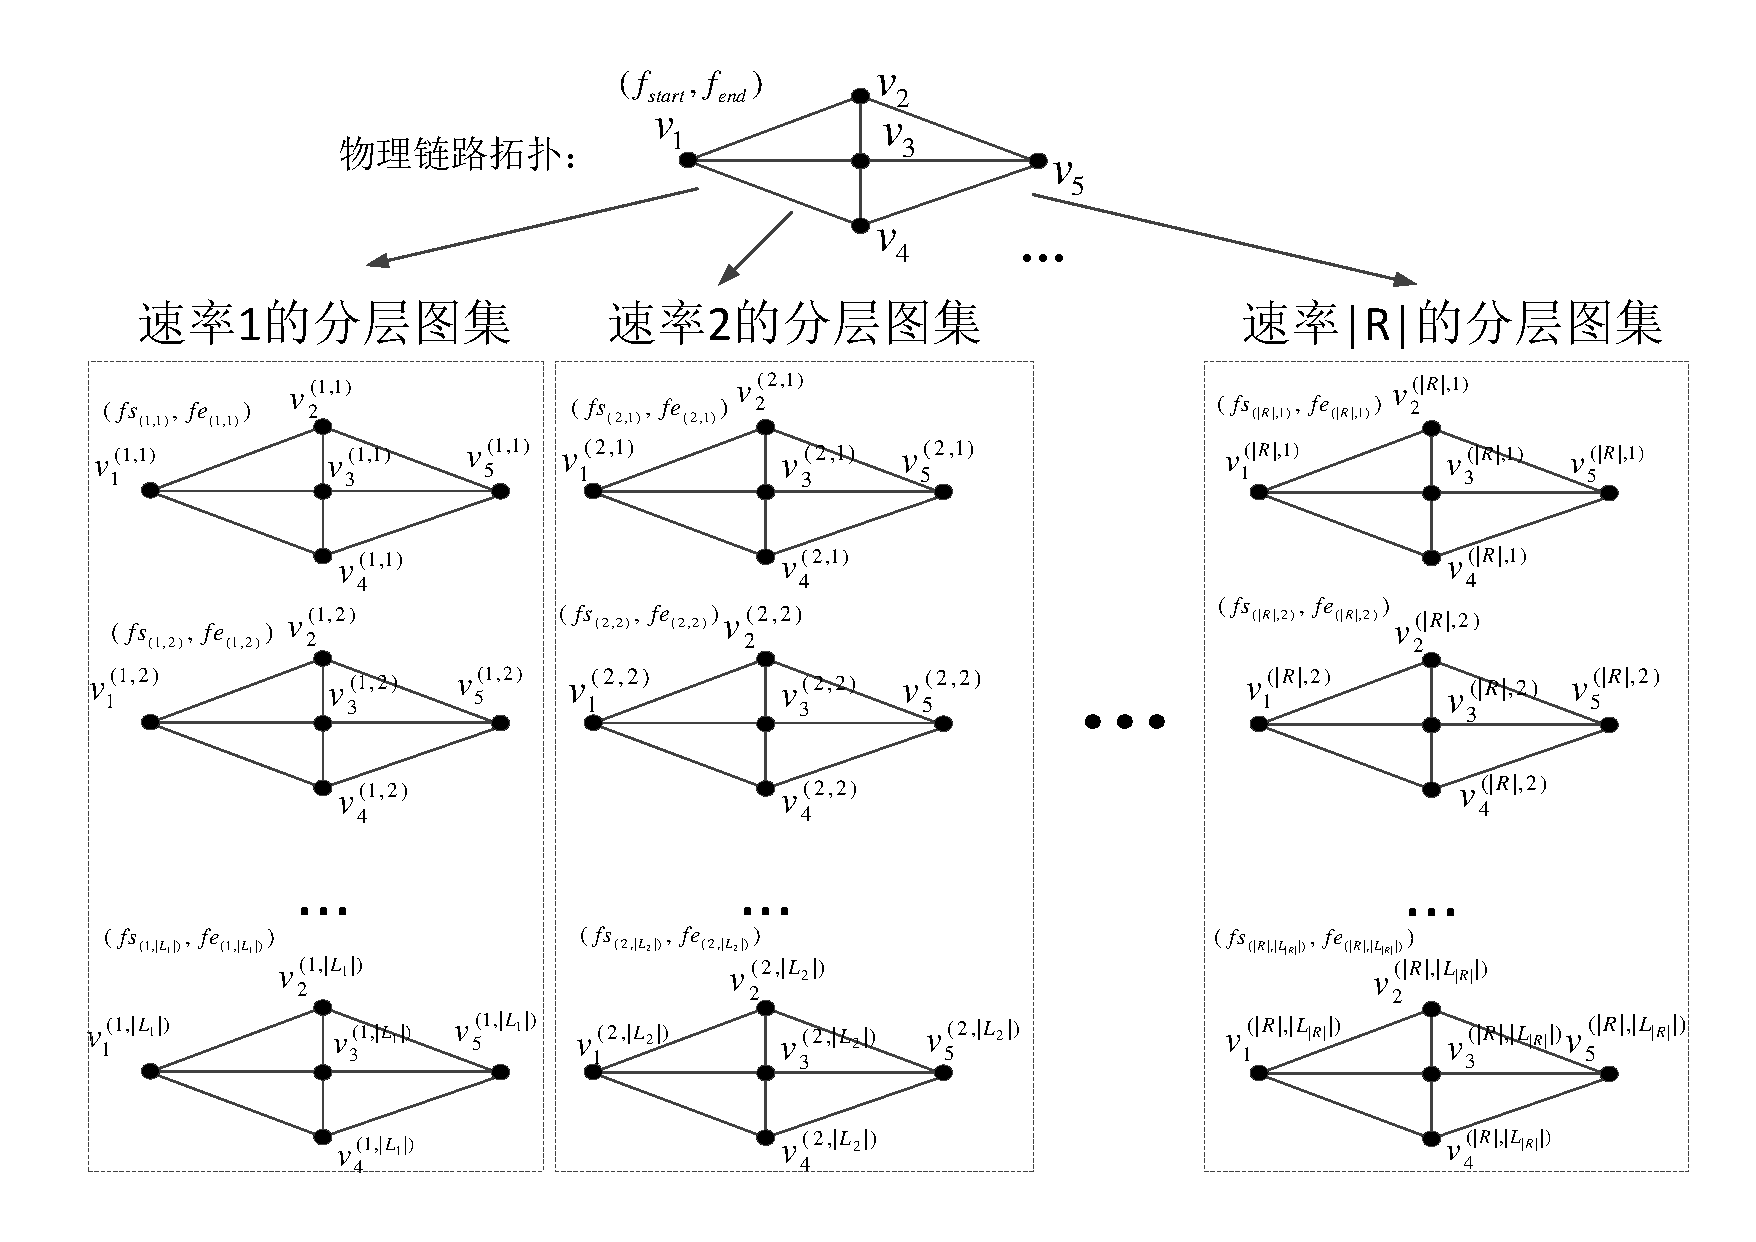
\includegraphics[width=1 \textwidth]{figures/LAYER.pdf}}
\end{center}
\caption{{\footnotesize{分层图示意}}}
\label{layer}
\end{figure*}
\section{主要优化流程}
根据前面的讨论,当一个速率为$r$的业务$TD_r(s,t)$到达网络时,一共有$L_r$ 个分层平面都可以用于此业务,也就是说如果在这些图当中都能为业务找到合适的路径的话,那么业务就有$L_r$ 条路径可供选择,我们可以选择代价最小的一条来优化路由。进一步,当有一批速率为$r$ 的业务集合$TD_r$到达网络时,如果大家都选择同一层加入的话,会出现大量的冲突,而且路由代价也会很大,但是由于现在有多个分层图平面可以选择,每个业务都有$L_r$条路径可以选择,这就给路由优化提供了可能,不同的业务需求可以选择不同层上的路径来进行路由,以使得总体路由代价减小,节省网络频谱资源,从而优化阻塞率。

本节提出一个基于分层图的动态RSA路由优化算法流程称为带路由优化的RSA算法(route optimization RSA,RORSA),算法流程如下图 \ref{bblayer}所示:
\begin{figure*}
\setlength{\belowcaptionskip}{-0.5cm}
\begin{center}
{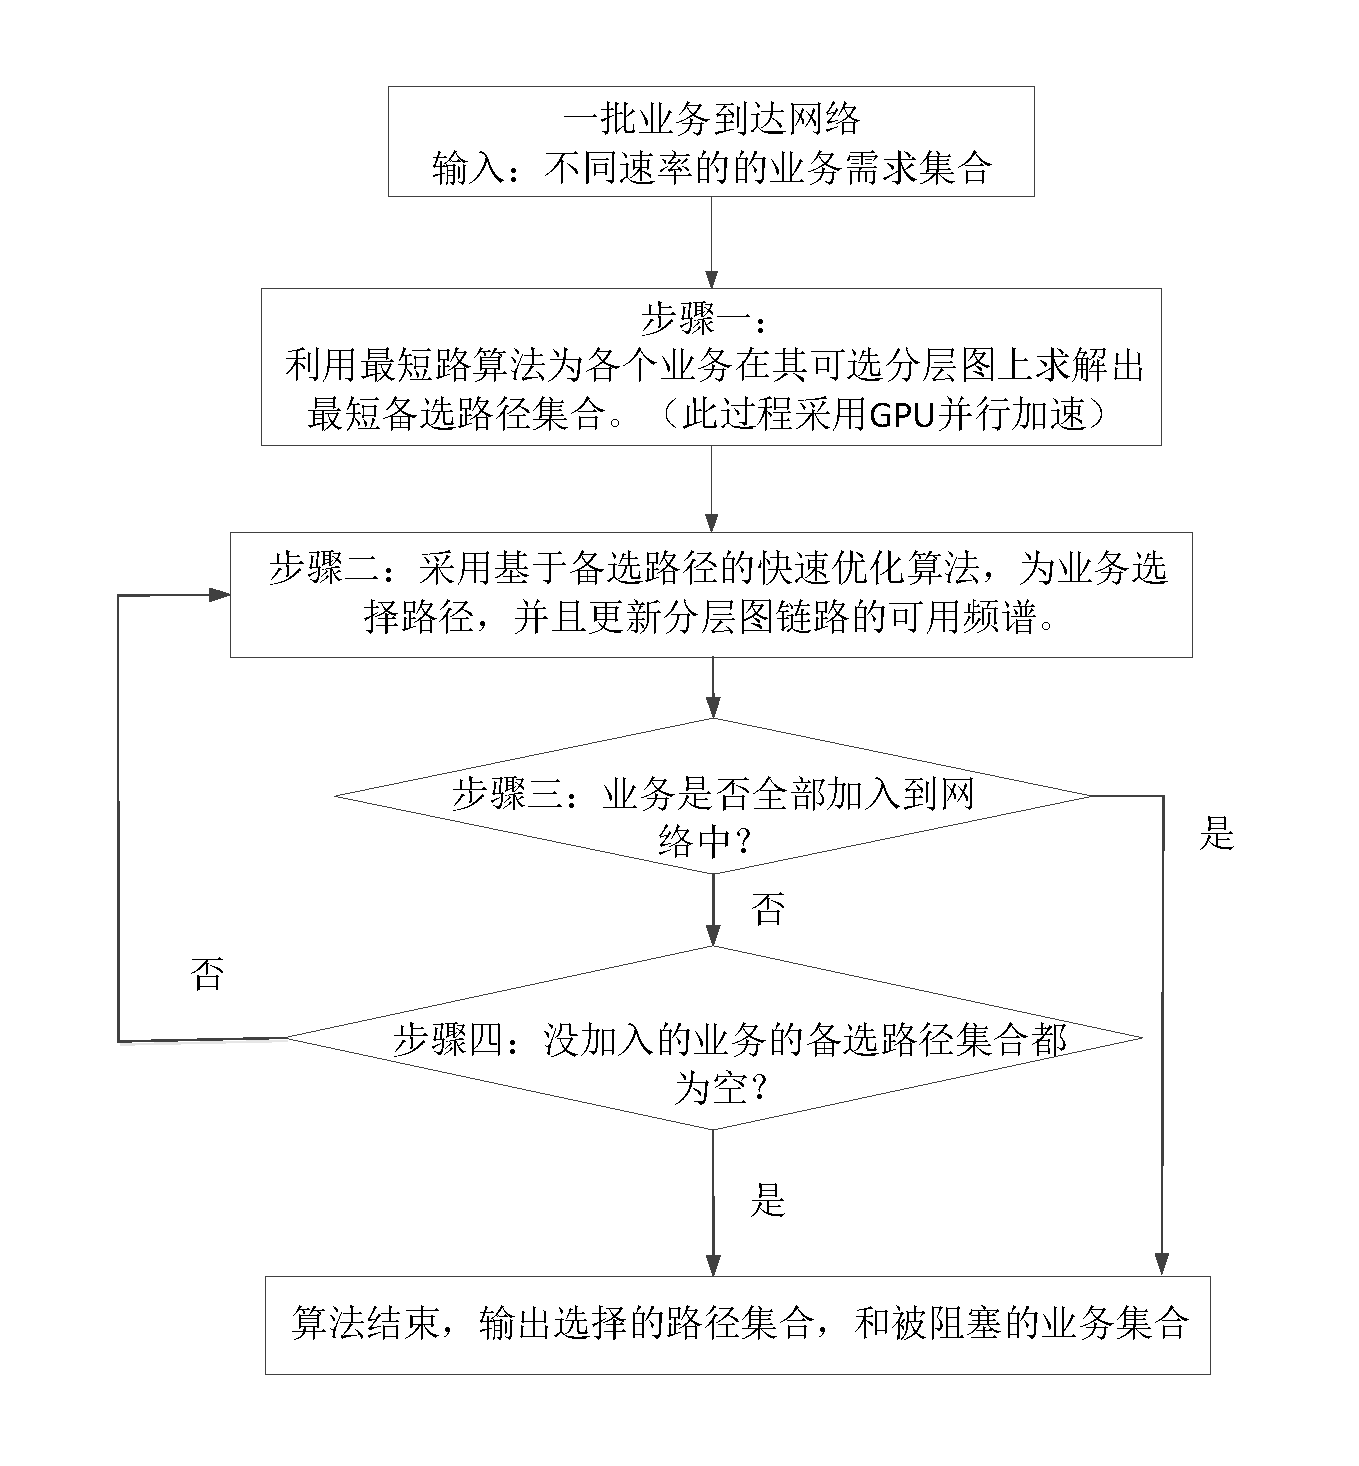
\includegraphics[width=1 \textwidth]{figures/bbprocess.pdf}}
\end{center}
\caption{{\footnotesize{算法优化流程}}}
\label{bblayer}
\end{figure*}
当一批业务到达网络时,对每一个业务在其对应速率的层上求出大量的备选路径,这个过程计算量较大,但是每一个拓扑层是独立的,所以可以采用并行算法来进行加速设计,后面4.4和4.5将讨论无权图和有权图上的两种基于GPU 的路由加速算法来加速这个步骤,当备选路径都求出来了之后采用一种快速路径选择算法来把业务安排进网络,这个步骤采用一种简单贪心的启发式算法,由于备选路径较多,实验发现这种简单的贪心算法已经可以很好的优化路径代价了。当业务的路径确定后,如果每个业务都能加入到网络,那么本轮算法结束,如果还有剩余的业务没有被安排进网络,需要判断业务的备选路径集合是否为空,如果为空,则说明所有层都不能为业务求出路径,业务将被阻塞;反之,如果业务的备选路径集合不是空,则说明业务是因为和其他业务的路径冲突而导致不能被安排进网络的,分层图中可能还存在其他可用路径,所以需要重新在分层图中计算路径,算法回到步骤二,对这些业务进行重新计算。

步骤一的具体算法将在4.4和4.5介绍,这里介绍步骤二的快速优化算法,快速优化算法的主要思想是根据求出来的备选路径为每个业务选择路径以使得整体路径代价最小,由于动态RSA环境下需要在短时间内安排好路径,所以为了提高计算速度,这里采用一种简单快速的贪心算法来进行解决,流程如算法\ref{arrange}所示。
\begin{algorithm}[htb]
\begin{algorithmic}[1]
\Require
$N(v,E)$:分层图;
$P$:备选路径集合;
$TD$:业务需求集合;
\Ensure
$AP$:加入业务的路径集合;
\For{$T \in TD$}
\State {对$P_T$中的路径按照路径的代价进行降序排序}
\EndFor
\State {对$T$按照$P_T$中的最小路径代价进行排序}
\For{$T \in TD$}
\For{$p \in P_T$}
\If{路径$p$所对应分层图上的相应链路没有被占用}
\State{把$p$加入到$AP$中,并更新$p$所对应的分层网络上的链路,跳出for循环,以继续为下一个业务选路}
\EndIf
\EndFor
\EndFor
\end{algorithmic}
\caption{路径选择算法}
\label{arrange}
\end{algorithm}

算法开始对每个业务的备选路径按照其代价进行降序排序,也就是每个业务优先会选择代价较低的备选路径。然后,再对业务按照其最小代价的路径进行排序,这样保证优先考虑代价小的业务。然后开始加入业务到网络,对每一个业务,遍历其已经排序好的备选路径,如果在相应分层图上路径包含的链路都是空闲的,则加入业务到网络中,更新分层图上的相应链路为占用状态,把这个路径$p$ 加入到集合$AP$ 中。最后算法输出路径集合$AP$, 算法结束。
\section{无权图情况下的GPU算法设计}

无权图情况下,路由的代价就是路径的跳数,跳数越少说明占用的网络资源越少,尽量优化路径的跳数可以节省网络资源,进一步的降低动态情况下的网络的阻塞。无权图情况下的路由算法一般使用BFS (宽度优先搜索)算法进行求解,BFS 算法从目的节点最近的点开始,一层一层的进行扩展直到找到目的节点,每扩展一层跳数增加一跳,扩展一层需要遍历大量的边,这些边的扩展操作是相互独立的,所以为算法提供了并行设计的可能性,在加上不同速率不同层上的路由求解上的并行,总体并行粒度是很大的,下面分别对不同的并行层次的设计进行讨论。
\subsection {相同速率业务的并行}

如下图\ref{bfs}所示,对速率都为$r$的一批业务,在其可用的每个分层图上并行进行计算,在每个分层图上,具有相同源节点的业务组成业务组,因为他们的路径可以一起计算,对每一个业务组,在GPU 上开辟$|E|$个线程对每一条边进行扩展操作,那么整个过程的的并行粒度为$|L_r||D_r||E|$,其中$|D_r|$为速率为$r$的业务组数量。
\begin{figure*}
\setlength{\belowcaptionskip}{-0.5cm}
\begin{center}
{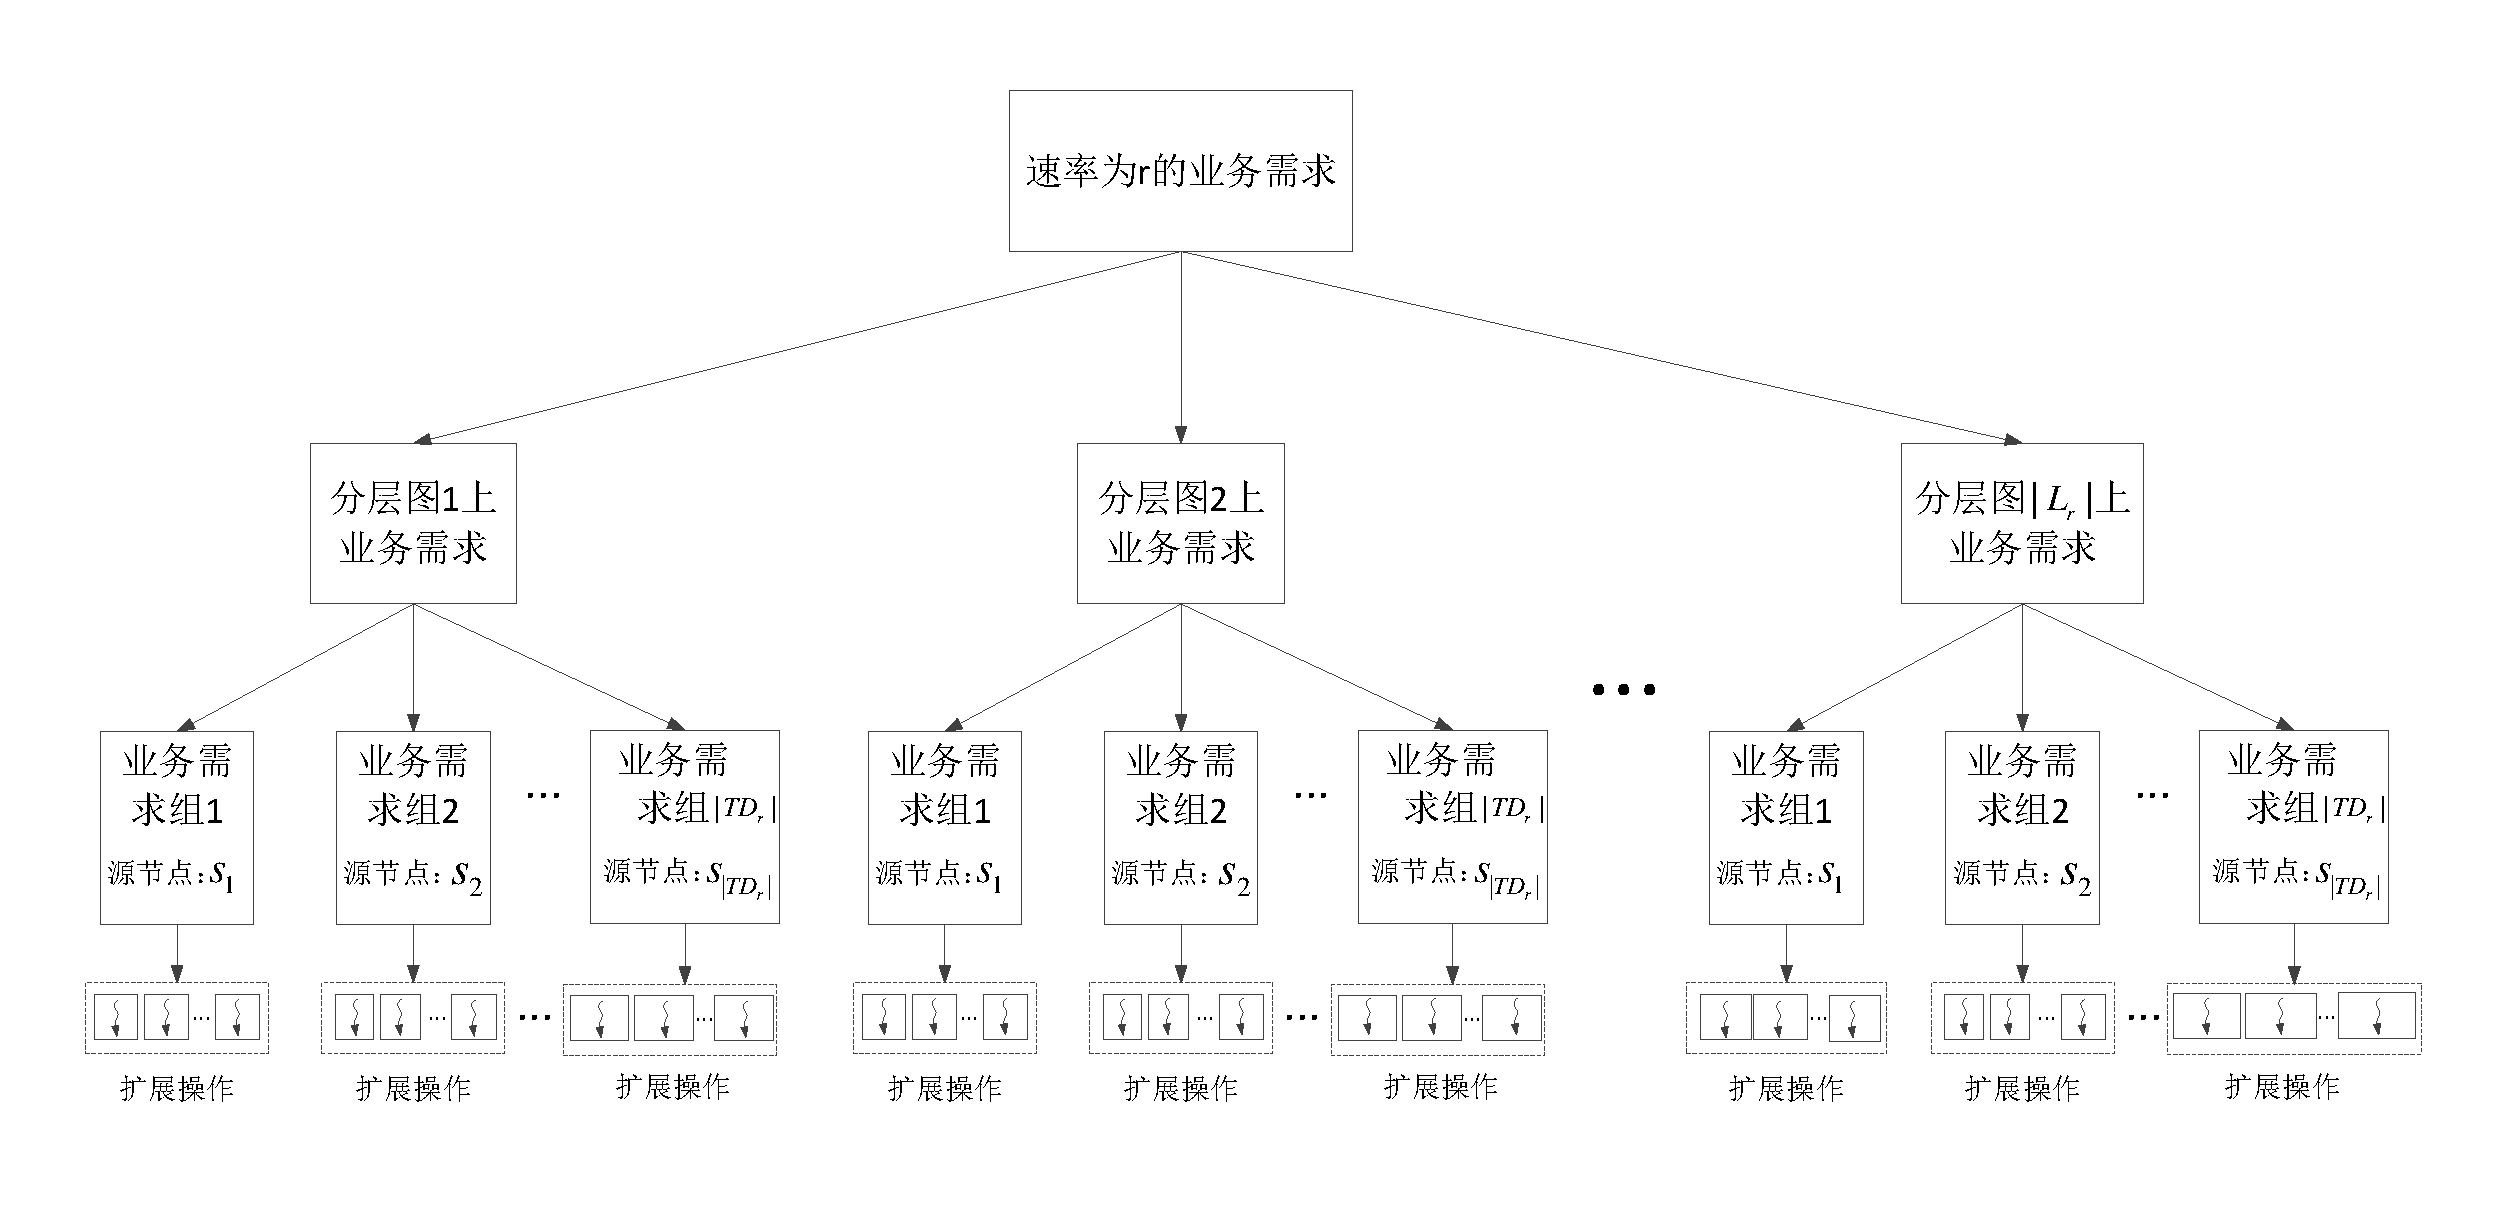
\includegraphics[width=1 \textwidth]{figures/bfs.pdf}}
\end{center}
\caption{{\footnotesize{bfs并行示意图}}}
\label{bfs}
\end{figure*}
\subsection{不同速率间业务的并行}
由于动态业务情况下每次到达网络的业务数和速率情况都是变化的,不同速率之间业务的并行不容易直接实现在一个kernel 中进行,我们采用GPU提供的流并行进行并行设计。如下图 \ref{bfssteam}所示:
\begin{figure*}
\setlength{\belowcaptionskip}{-0.5cm}
\begin{center}
{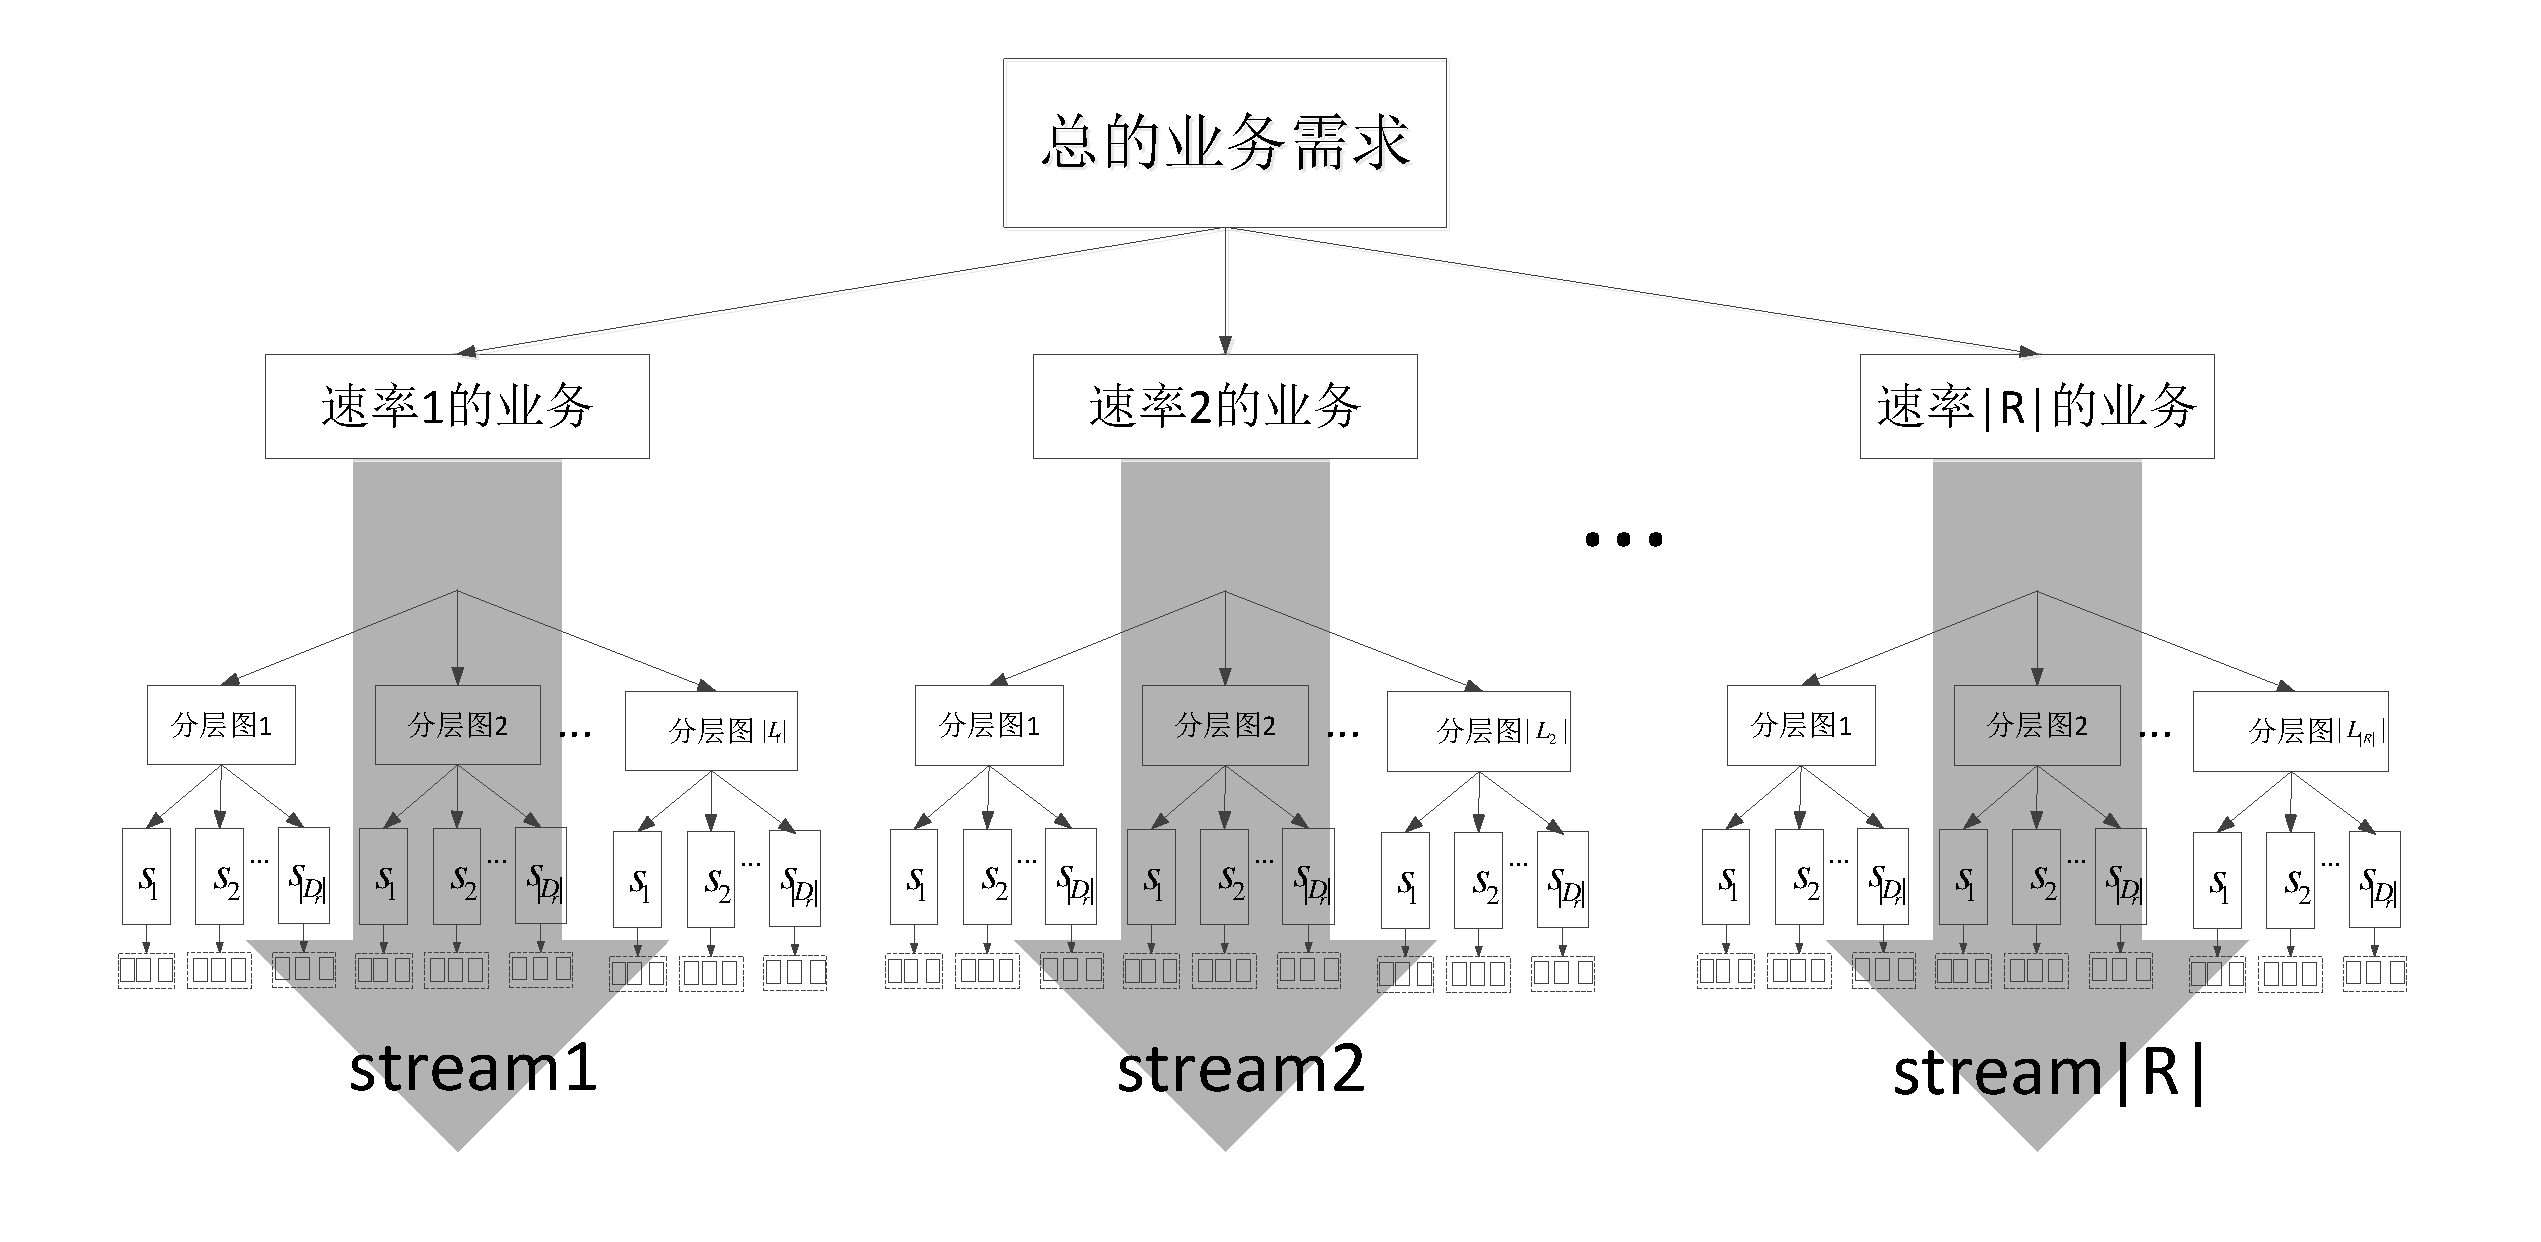
\includegraphics[width=1 \textwidth]{figures/hbfs.pdf}}
\end{center}
\caption{{\footnotesize{bfs流并行示意图}}}
\label{bfssteam}
\end{figure*}
我们为每一个速率建立一个stream来负责这个速率的业务计算,假设业务一个有$|R|$个不同速率,那么需要建立$|R|$个stream,多个kernel 同时执行,充分利用GPU 的SMIT资源,当SIMT资源足够时,每个kernel将并行执行,当SIMIT不足时,不同的kernel之间可以进行快速的切换,以达到隐藏延迟的效果。

\subsection{GPU上kernel设计}
和3.4.2中讨论不一样,在BFS的并行中不会存在前驱节点更新的同步问题,但是,我们依然需要两个kernel函数,这是因为扩展kernel 需要执行多次,如果扩展和更新同时执行,那么更新也会执行多次,这会增多内存访问,所以我们把两个操作分成两个kernel,一个$kernel\_BFS\_extend$ 进行边的扩展操作,一个$kernel\_BFS\_update$ 进行前驱节点的更新操作,其中$kernel\_BFS\_extend$需要多次调用,但是$kernel\_BFS\_update$ 只需要在最后执行一次。
\begin{algorithm}[t]
\begin{algorithmic}[1]
\Function{kernel\_BFS\_extend}{$E$, $Dist$,$rid$,$round$}
\State {$bid \leftarrow$ block ID}
\State {$tid \leftarrow$ thread ID}
\State {用$(bid,tid,rid)$ 映射到边的标号$eid$}
\State {用$(bid,tid,rid)$ 映射到分层图标号$lid$}
\State {$e \leftarrow E[gid][eid]$}
\If {$e.avaliable==-1$}
\State{return}
\EndIf
\State {用$(bid,tid,rid)$ 映射到的源点标号$sid$}
\If{$Dist[lid][sid][e.head]>round $\&\&$ Dist[lid][sid][e.tail]+1==round$}
\State {$Dist[gid][sid][e.head] \leftarrow round$}
\EndIf
\EndFunction
\end{algorithmic}
\caption{kernel\_BFS\_extend}
\label{KernelBFS}
\end{algorithm}
在$kernel\_BFS\_extend$中,输入$E$是所有的分层图的边所组成的集合,$Dist$是预先分配的距离标记数组,他是一个三维数组,第一维表示当前距离数组对应的分层图标号,第二维度表示源节点,第三维度表示目的节点,比如$Dist[3][10][5]=4$表示在第3个分层图上,点10到3的距离为4。初始时,除了源节点距离被初始化为0之外,其他的距离都被初始化为无穷大。$rid$表示当前kernel 负责计算的业务速率标号,他是区分不同流的标记,$rid$不同表示执行kernel的流不同。$round$ 表示当前扩展的层数,由于BFS是一层一层进行扩展操作,我们需要记录当前层数来决定哪些边需要扩展。算法开始时先进行一系列映射操作,将线程映射到边标号$eid$,当前所在分层图标号$lid$,以及源节点标号$sid$。 由于动态情况下,边的可用状态可能发生变化,找到边之后,需要判断这条边是否可用,如果不可用则返回。接着判断当前边是否可以进行扩展操作,如果尾节点已经更新过了($Dist[lid][sid][e.head]<=round$),则不能再更新了,反之,还需要判断头节点是否是上一次扩展层的节点($Dist[lid][sid][e.tail]+1==round$),如果是的话,那么就更新尾节点的距离为当前扩展层$round$。
\begin{algorithm}[t]
\begin{algorithmic}[1]
\Function{kernel\_bfs\_update}{$E$, $Pre$,$rid$}
\State {$bid \leftarrow$ block ID}
\State {$tid \leftarrow$ thread ID}
\State {用$(bid,tid,rid)$ 映射到边的标号$eid$}
\State {用$(bid,tid,rid)$ 映射到分层图标号$lid$}
\State {$e \leftarrow E[gid][eid]$}
\If {$e.avaliable==-1$}
\State{return}
\EndIf
\State {用$(bid,tid,rid)$ 映射到的源点标号$sid$}
\If{$Dist[lid][sid][e.head]==Dist[lid][sid][e.tail]+1$}
\State {$Pre[gid][sid][e.head] \leftarrow e.tail$}
\EndIf
\EndFunction
\end{algorithmic}
\caption{kernel\_BFS\_update}
\label{KernelBFS}
\end{algorithm}
在$kernel\_BFS\_update$中,其主要逻辑和$kerne\l_BFS\_extend$一样,在进行更新判断的时候,判断当前边的头节点是否是尾节点的上一层(Dist[lid][sid][e.head]==Dist[lid][sid][e.tail]+1)如果是的话,那么头节点就有资格作为尾节点的前驱节点,于是进行前驱更新操作。
介绍完了两个kernel之后,算法 \ref{ParaSPC}为整个并行BFS的算法流程:
\begin{algorithm}[t]
\begin{algorithmic}[1]
\Require
业务需求集合$TD$;
分层图链路集合$E$;
\Ensure {业务需求的最短路径集合$P$}
\State {将业务根据速率和源节点重新组合成业务分组集合$D$}
\For {$D_r \in D$}
\For {$d_{rs} \in D_r$}
\For {$l \in L_r$}
\For {$v \in V$}
\If {$v==s$}
\State {$Dist[l][s][v]\leftarrow$ 0}
\Else
\State {$Dist[l][s][v]\leftarrow \infty $}
\EndIf
\State {$Pre[l][s][v]\leftarrow -1 $}
\EndFor
\EndFor
\EndFor
\EndFor
\State {新建$|R|$个流,组成集合$S$}
\State {$round \leftarrow$ 1}
\While{$round<=W_{max}$}
\For{r in R}
\State {在流$S_r$上发射 kernel\_bfs\_extend($E$, $Dist$,$r$,$round$)}
\EndFor
\State{round=round+1}
\EndWhile
\For{r in R}
\State {在流$S_r$上发射 kernel\_bfs\_update($E$, $Dist$,$r$,$round$)}
\EndFor
\State {根据前驱数组$Pre$重建路径,然后把路径加入到集合$P$}
\end{algorithmic}
\caption{{并行BFS计算}}
\label{ParaSPC}
\end{algorithm}
算法 \ref{ParaSPC}开始时先将业务按照速率的不同进行划分,再将业务按照源节点的不同划分成不同的业务组集合$D$,比如,$D_r \in D$表示速率为$r$的业务组集合,$d_{rs} \in D_r$ 表示速率为$r$的源节点标号为$s$的业务组。划分好业务组之后,就开始初始化距离数组,将速率对应的所有分层图上的源节点距离初始化为0,这是一个三层的for 循环,第一层遍历速率标号,第二层遍历源节点标号,第三层遍历速率所对应的分层图标号。初始化$Dist$数组后,在发射kernel之前需要先新建$|R|$个GPU流,不同的流将对不同速率的业务进行计算。$round$ 为扩展的层数标记,开始时$round$初始化为1。while 循环中进行扩展操作,其中$W_{max}$为跳数限制,最大跳数不能超过$W_{max}$,每一次扩展操作只会使得路径长度增加一跳,所以最多只能循环$W_{max}$次。while循环中for循环用来发射不同的流,因为发射不同流的kernel是异步操作,for循环不会去等待上一个kernel结束了才去执行下一个kernel,所以可以认为所有kernel都是同时间发射的。while循环结束后,算法发射$kernel\_BFS\_update$进行前驱节点记录操作,最后根据这些前驱信息,算法重新恢复出路径,组成路径集合$P$,算法结束。
\section{带权图情况下的GPU算法设计}

在实际应用场景中,我们常常需要将不同的链路设置为不同的代价,因为链路的延迟,租用费用可能不同,所以有必要考虑链路带权情况下的优化设计,算法优化的目标是业务使用的链路总体代价最小化,为了简化问题模型,本节只讨论链路代价为正值的情况。本节将逐步分析和设计适用于带权图的分层网络GPU并行算法。
\subsection{带跳数限制的最短路算法}
带跳数约束的BFS路由,由于没有考虑链路的权重差异,把所有链路的权重看作一样,所以FS路由的优化目标就是跳数,BFS就是寻找跳数最短的路径,跳数约束只是使得BFS算法提前结束。但是在带权的链路情况下,路由的优化目标是最小化链路代价和,也就是寻找一条代价最小的满足跳数约束的路径,跳数越短并不意味则代价越小,代价越小也不意味着跳数越小,这使得带权情况下比无权情况更加复杂。

为了说明带权带跳数约束下的路由算法,我们介绍一些符号,在图$N(V,E)$中,有点$i \in V$, 和点$j \in V$,假设集合$P_{ijk}$ 表示点$i$到点$j$的所有跳数为$k$的路径所组成的集合,设$p_{ijk}^*$为集合$P_{ijk}$当中代价最小的那一条路径,即$p_{ijk}^* =\arg\min\limits_{p \in P_{ijk}}\{Price\_Of(p)\}$,我们设最小代价数组为$Price$,$Price$为三维数组,其中$Price[i][j][k]=Price\_Of(p_{ijk}^*) )$,即$Price[i][j][k]$表示为$p_{ijk}^*$ 的代价,也就是说$Price[i][j][k]$ 表示$i$ 到$j$ 的跳数为$k$跳的最小代价路径的代价。对点$i$,边集合$PreE_i$表示点$i$ 的入边组成的集合,点集合$PreN_i$表示点$i$的入节点所组成的集合。

有了上面的符号介绍后,假设业务的源节点为$s$,下面给出一个动态规划递推式,其中$w_{nj}$ 表示边$(n,j)$ 的代价大小:
\begin{equation}\label{dynamic}
\begin{split}
Price[i][j][k]
=\begin{cases}
\min\limits_{n \in PreN_i}{Price[i][n][k-1]+w_{nj}} & \text{if $k>0$}\\
0 & \text{if $k=0$ and $i=s $} \\
\infty &{otherwise}
\end{cases}
\end{split}
\end{equation}

设$p_{ijk}^*$为点$i$到$j$的跳数为$k$的最小代价路径,由于点$j$的前驱节点只可能是那些属于集合$PreN_j$ 的点,点$j$ 的前驱边只可能是集合$PreE_j$ 中的某一条边,那么最优路径$p_{ijk}^*$中的第$k$条边一定属于集合$PreE_j$,于是递推式中我们遍历了这些边,另外,设经过边$e \in PreE_j$到达$j$的跳数为$k$的最优路径为$p_{ijk}^e$,那么根据Price的定义我们可以得到$Price\_Of(p{ijk}^e)=Price[i][e.head][k-1]+w_e$,其中,$e.head$表示边的头结点,也就是点$i$的对应于边$e$ 的前驱节点。那么最优路径$p_{ijk}^*=\arg\min\limits_{e \in PreE}{Price_Of(p_e)}$,相应的最优代价$Price[i][j][k]=\min\limits_{e \in PreE}{Price_Of(p_e)}$,也就是$\min\limits_{n \in PreN_i}{Price[i][n][k-1]+w_{nj}}$。 注意边界情况下($k==0$),由于除了源节点自己之外,源节点到其他节点的跳数不可能是零,所以开始时需要设置代价为无穷大,而源节点到他自己距离设置为0。

上面的动态规划递推式可以求得一个点到任意点的跳数为1到$k$的最优路径,而我们是要求得在跳数限制下的最优代价路径,我们需要对求得的动态规划解进行处理,设二维数组$OPCost$表示跳数限制下的最优路由代价值,那么跳数限制约束下的点$i$到点$j$的最小代价路径的代价为$OPCost[i][j]$,可以得到下面的表达式:
\begin{equation}\label{best}
\begin{split}
OPCost[i][j]=\min\limits_{k \in W_{max}}{Price[i][j][k]}
\end{split}
\end{equation}

假设满足跳限约束的最优代价路径为$p_{ij}^*$,假设路径$p_{ij}^*$的跳数为$h$,$h \in [1,W_{max}]$,显然$p_{ij}^*=p_{ijh}$,但是实际上我们并不知道$h$ 的值,所以我们从$[1,W_{max}]$ 对$h$进行遍历,那么$p_{ij}^*$肯定是其中代价最小的一条,所以$p_{ij}^*=\min\limits_{k \in W_{max}}{Price_Of(p_{ijk}^*)}$,同样,$OPCost[i][j]=\min\limits_{k \in W_{max}}{Price[i][j][k]}$。

观察动态规划递推式,可以看到,在递推过程不会去记录路径,这样求得路径可能会经过重复的点,但是,最优路径$p_{ij}^*$ 中是不可能经过重复节点的,下面本文进行证明。首先,路径跳数$h<4$ 的路径是不可能经过重复的节点,我们讨论$h>=4$时的情况,如果路径重复经过了一个点,那么路径中一定存在一个环,如下图 \ref{prof},这个存在环的路径为$L_1-L_2-L_3-L_2-L_4$,假设链路$L_2$ 的跳数为$h_2$,代价为$C_2$,由于链路的代价都是正数,所以$C_2>0$,那么存在一条跳数为$t=h-h_2$ 的,代价为$OPCost[i][j]-C_2$ 的由$i$ 到$j$ 的路径$L_1-L_2-L_4$,而这条路径的代价肯定小于等于$Price\_Of(p_{ijt})$,即$OPCost[i][j]-C_2<=Price\_Of(p_{ijt})<=OPCost[i][j]$,进一步得到$OPCost[i][j]-C_2<=OPCost[i][j]$,这与$C_2>0$矛盾,所以最优路径不可能经过重复的节点。
\begin{figure*}
\setlength{\belowcaptionskip}{-0.5cm}
\begin{center}
{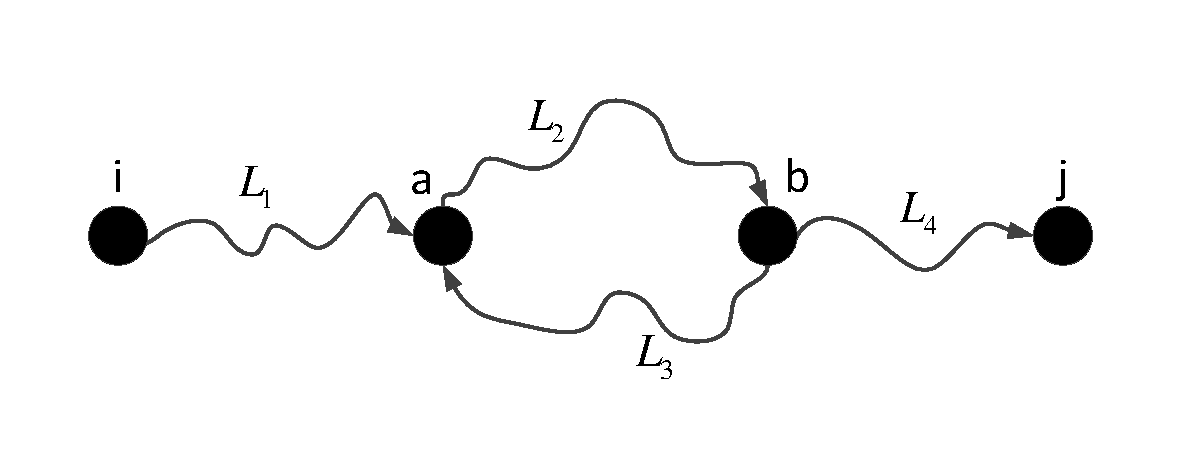
\includegraphics[width=1 \textwidth]{figures/circle.pdf}}
\end{center}
\caption{{\footnotesize{无环证明}}}
\label{prof}
\end{figure*}
\subsection{并行层次}
\subsection{并行动态规划算法}

上一节提出了动态规划模型,证明了算法的正确性,本节我们讨论这个动态规划算法在GPU上的并行设计框架,以及分层图和不同速率的并行层次设计。单个图上的动态规划的串行执行过程如下伪代码所示:
\begin{algorithm}[t]
\begin{algorithmic}[1]
\Require
点的入边集合$PreE$;
点的入点集合$PreN$;
源节点$s$;
\Ensure {最优代价数组$Price$;最优前驱节点数组$Pre$;}
\For {$k \in [1,W_{max}]$}
\For {$v \in V$}
\State {Price[s][v][k]=$\min\limits_{n \in PreN_v}{Price[s][n][k-1]+w_{nv}}$}
\State {Pre[i][j][k]=$\arg\min\limits_{n \in PreN_v}{Price[s][n][k-1]+w_{nv}}$}
\EndFor
\EndFor
\end{algorithmic}
\caption{{串行动态规划算法}}
\label{pda}
\end{algorithm}

算法循环$W_{max}$次,每一次循环中对每一个点进行对应的$Price$数组进行更新,而这些更新操作是相互独立的,所以,可以进行并行设计,对每一个点的$Price$ 数组更新操作开辟一个线程进行计算,这个线程遍历当前点的前驱边,寻找最优的那一条前驱边,这里的并行粒度只有图的点数$|N|$,但是考虑到不同个业务和不同的分层图上计算也是并行的,总的并行粒度为$|N||D||R|$,这样需要开辟大量的线程,充分利用GPU上的SIMT计算资源。

下面考虑单个速率情况下的并行框架,如下图 \ref{DRK}所示,动态规划算法和BFS单个速率情况下的并行类似,只是BFS那里的对每一条边并行的扩展操作被替换成了对每一个点并行的$Price$数组更新操作。
\begin{figure*}
\setlength{\belowcaptionskip}{-0.5cm}
\begin{center}
{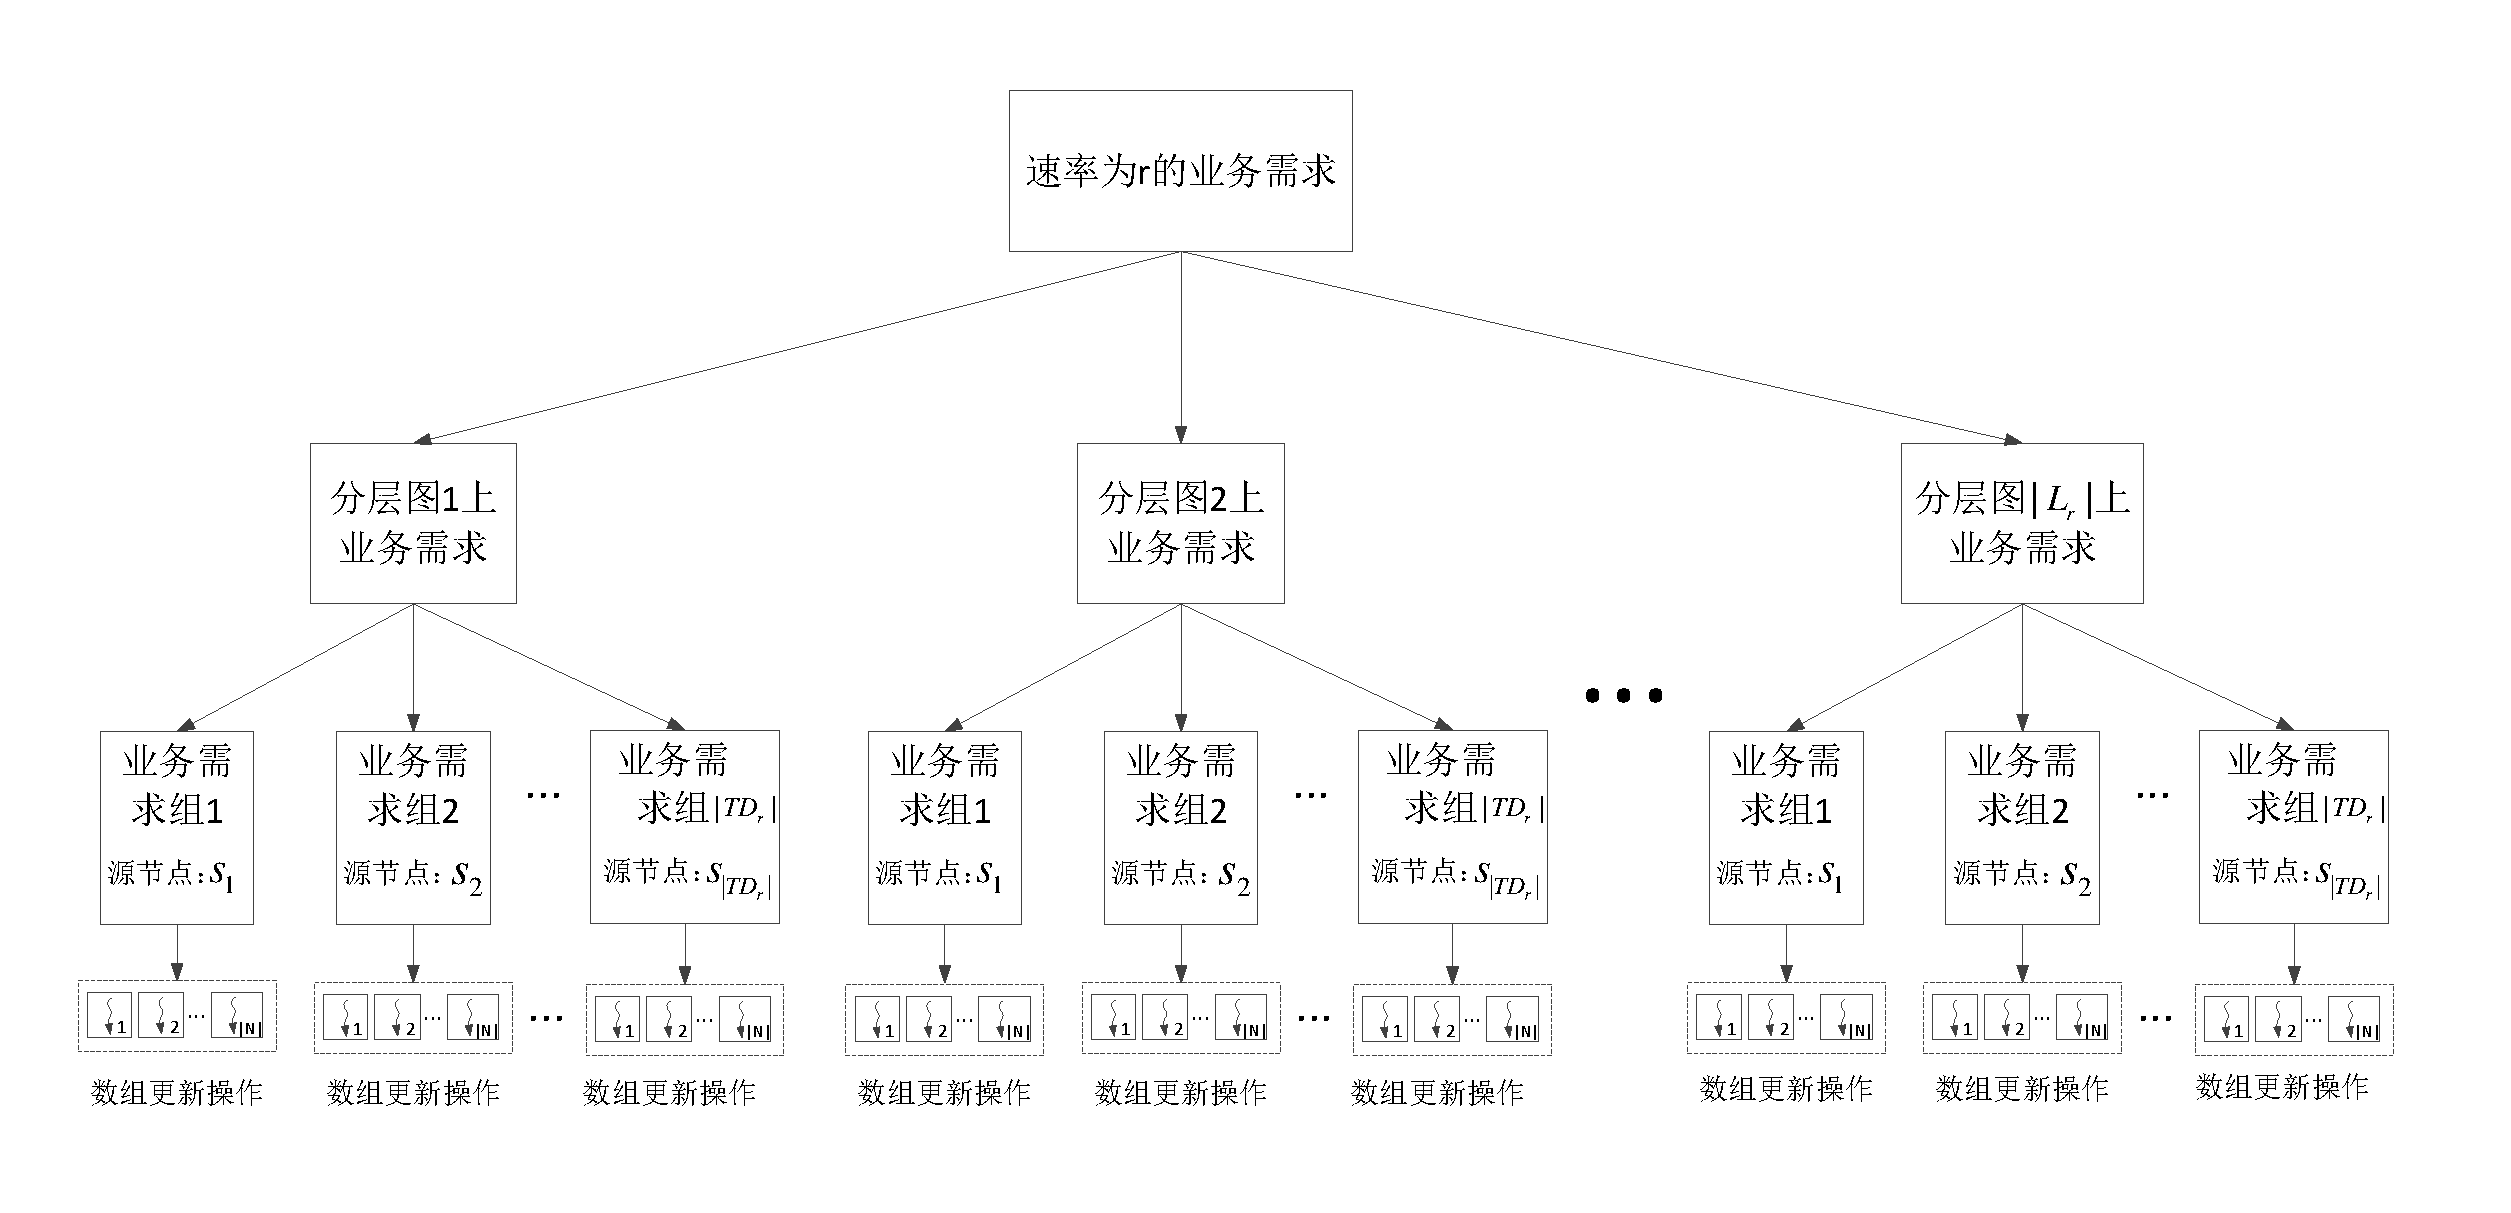
\includegraphics[width=1 \textwidth]{figures/DRK.pdf}}
\end{center}
\caption{{\footnotesize{动态规划并行示意图}}}
\label{DRK}
\end{figure*}

和BFS一样,对不同速率的业务,本文依然采用不同的流进行并行,其并行过程如下所示:
\begin{figure*}
\setlength{\belowcaptionskip}{-0.5cm}
\begin{center}
{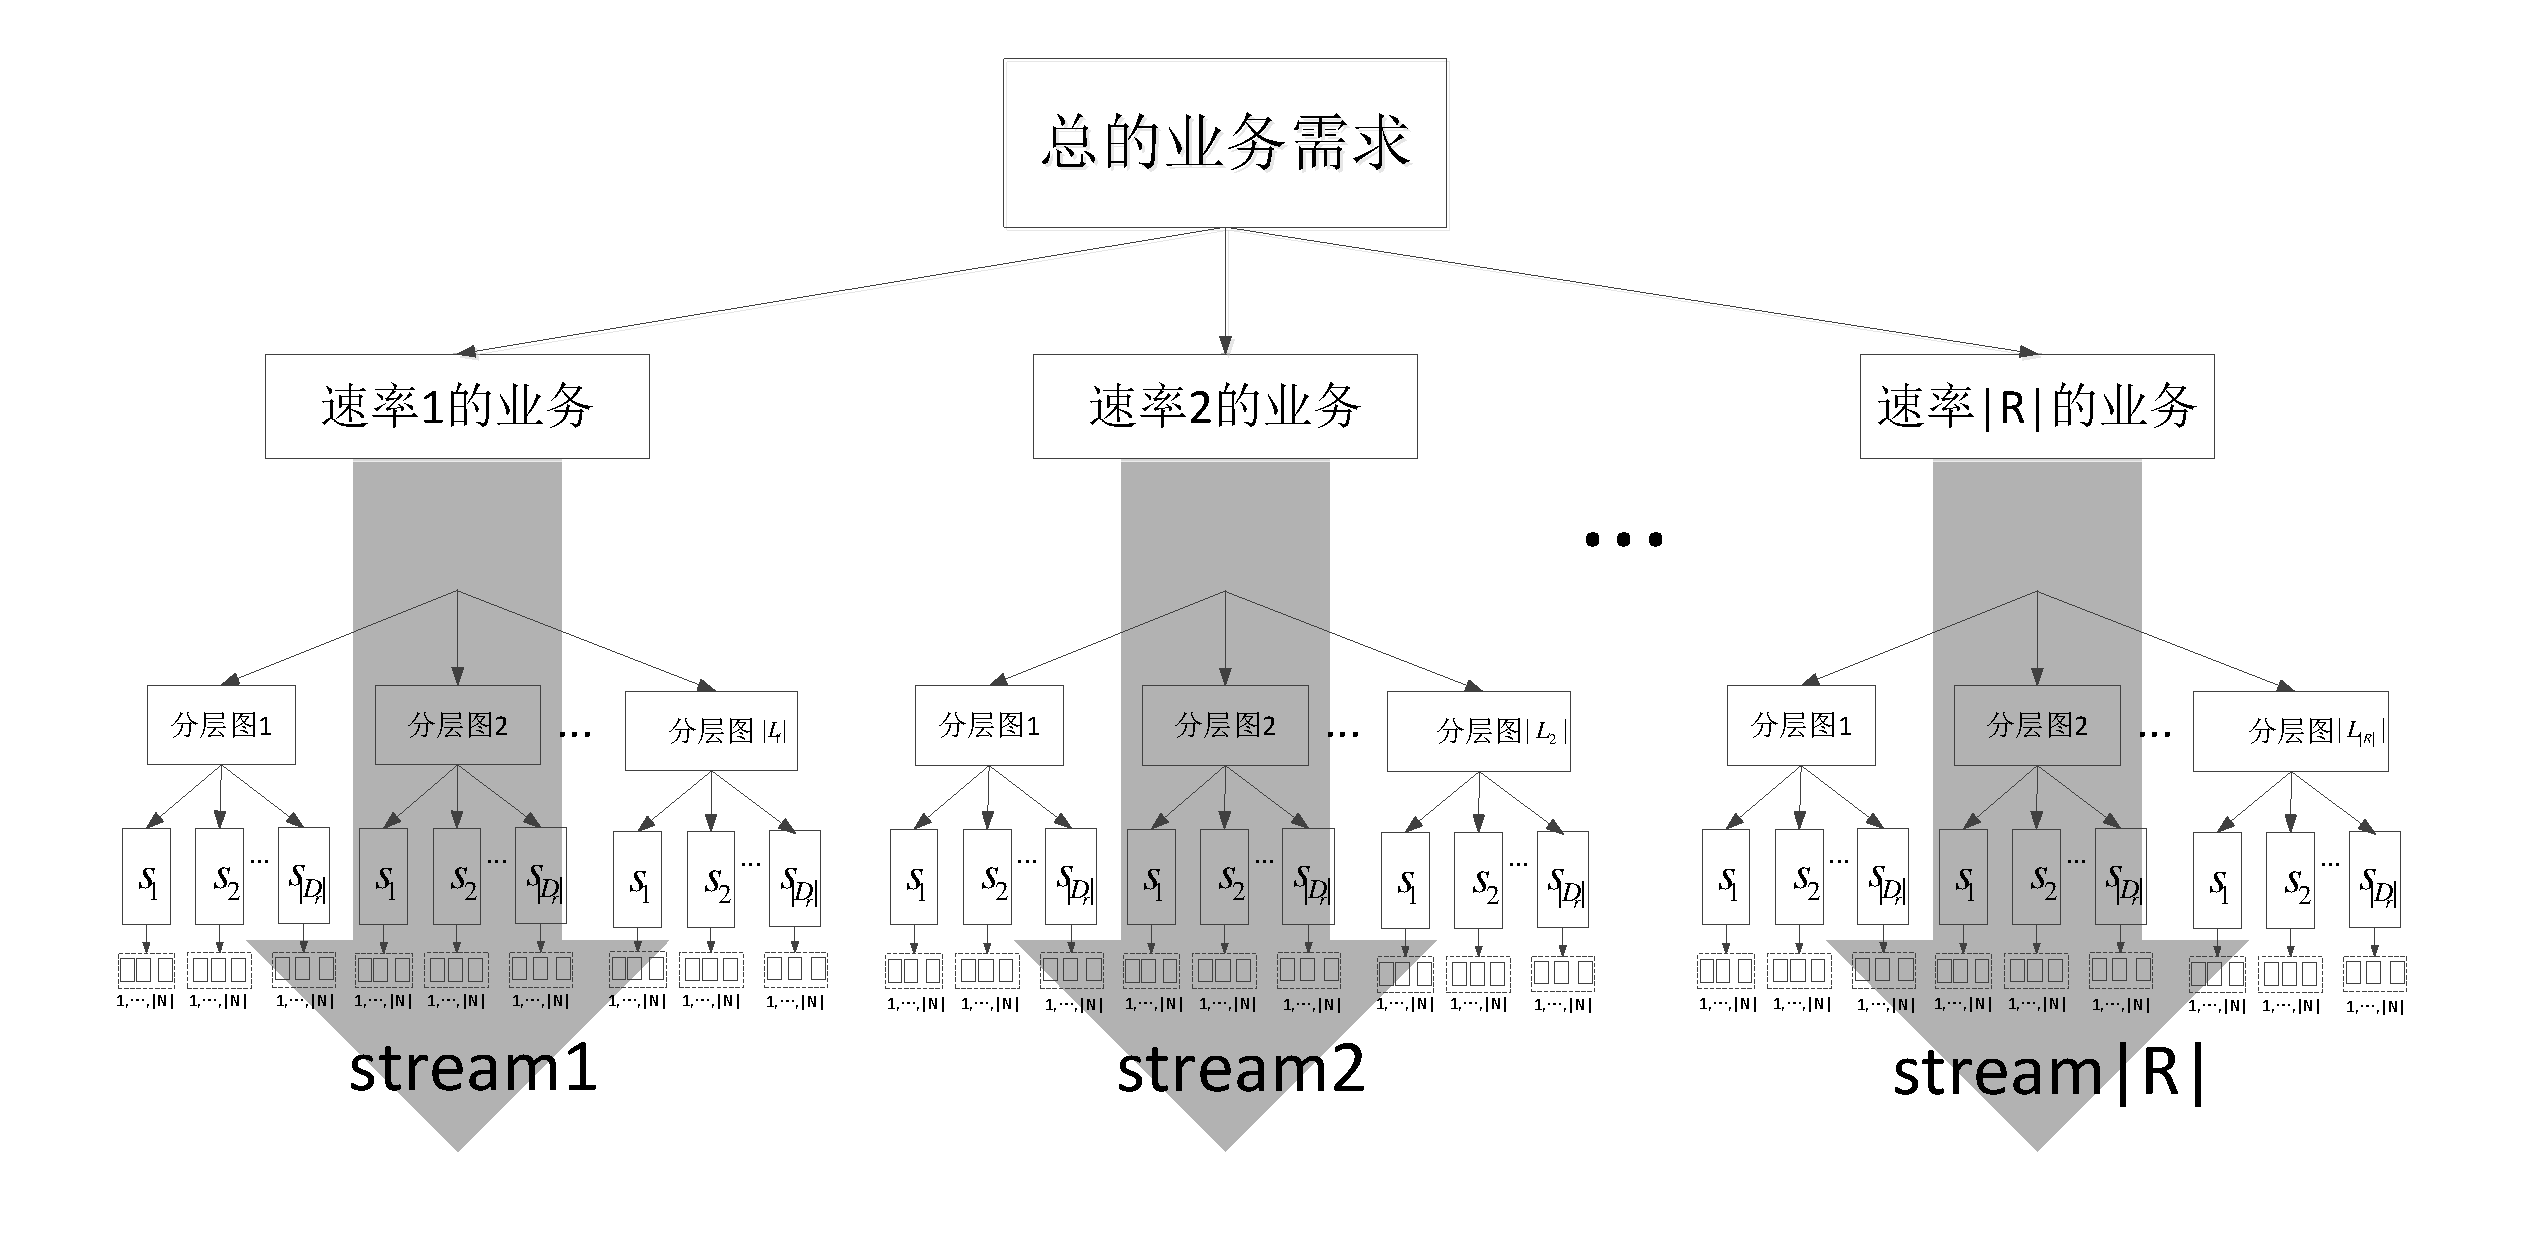
\includegraphics[width=1 \textwidth]{figures/BBK.pdf}}
\end{center}
\caption{{\footnotesize{动态规划流并行示意图}}}
\label{prof}
\end{figure*}
\subsection{GPU上kernel设计}
动态规划的GPU代码设计如下:
\begin{algorithm}[t]
\begin{algorithmic}[1]
\Function{kernel\_dynamic\_update}{$PE$,$rid$,$k$}
\State {$bid \leftarrow$ block ID}
\State {$tid \leftarrow$ thread ID}
\State {用$(bid,tid,rid)$ 映射到边点的标号$nid$}
\State {用$(bid,tid,rid)$ 映射到边源节点的标号$sid$}
\State {用$(bid,tid,rid)$ 映射到分层图标号$lid$}
\For {$e \in PE[lid][nid]$}
\If{$e.avalible>0$}
\If {$Price[lid][sid][nid][k]<Price[lid][sid][e.s][k-1]+e.weight$}
\State{$Price[lid][sid][nid][k]=Price[lid][sid][e.s][k-1]+e.weight$}
\State{$Pre[lid][sid][nid][k]=e.s$}
\EndIf
\EndIf
\EndFor
\EndFunction
\end{algorithmic}
\caption{kernel\_dynamic\_update}
\label{KernelDynamic}
\end{algorithm}
在$kernel\_dynamic\_update$中,输入$PE$是一个二维的集合数组,比如,$PE[2][3]$表示第2个分层图上点3 的入边集合。$Price$ 是预先分配的代价数组,他是一个三维数组,第一维表示当前代价数组对应的分层图标号,第二维度表示源节点,第三维度表示目的节点,第四维度表示路径的跳数,比如$Price[4][3][10][5]$=7 表示在第4个分层图上,点3到10的跳数为5的最优路径代价为7,初始时,当跳数等于0 时,除了源节点代价被初始化为0之外,其他的距离都被初始化为无穷大。
$Pre$数组是前驱数组用以记录前驱信息来恢复路径,$Pre$数组和$Price$数组一样,是一个四维数组,$Pre[4][3][10][5]$=50表示在第4个分层图上,点3到10的跳数为5的最优路径的前驱节点(也就是路径上的倒数第二个点)为点50。$rid$表示当前kernel 负责的计算的业务速率标号,他是区分不同流的标记,$rid$ 不同表示执行kernel的流不同。$k$ 表示当前扩展的层数,也就是跳数。算法开始时先进行一系列映射操作,将线程映射到点标号$eid$,当前所在分层图标号$lid$,以及源节点标号$sid$,映射完成后就可以进行Price数组的更新了,也就是要去寻找最优的入边,算法遍历点的所有入边,由于动态情况下,边的可用状态可能发生变化,找到边之后,需要判断这条边是否可用,如果不可用则跳过这条边,反之,就判断更新条件是否成立($Price[lid][sid][nid][k]<Price[lid][sid][e.s][k-1]+e.weight$),如果条件成立则说明这条入边比之前的要好,经过这条边到达当前点的路径代价更小,所以要更新Price数组,同时为了后面恢复路径需要记录前驱信息在数组$Pre$中。
\begin{algorithm}[t]
\begin{algorithmic}[1]
\Require
业务需求集合$TD$;
各个分层图前驱链路集合$PE$;
\Ensure {业务需求的最短路径集合$P$}
\State {将业务根据速率和源节点重新组合成业务分组集合$D$}
\For {$D_r \in D$}
\For {$d_{rs} \in D_r$}
\For {$l \in L_r$}
\For {$v \in V$}
\If {$v==s$}
\State {$Price[l][s][v][0]\leftarrow$ 0}
\Else
\State {$Price[l][s][v][0]\leftarrow \infty $}
\EndIf
\State {$Pre[l][s][v][0]\leftarrow -1 $}
\EndFor
\EndFor
\EndFor
\EndFor
\State {新建$|R|$个流,组成集合$S$}
\State {$k \leftarrow$ 1}
\While{$k<=W_{max}$}
\For{r in R}
\State {在流$S_r$上发射 kernel\_dynamic\_update($PE$,$rid$,$k$)}
\EndFor
\State{k=k+1}
\EndWhile
\State {根据前驱数组$Pre$重建路径,然后把路径加入到集合$P$}
\end{algorithmic}
\caption{{并行动态规划的计算}}
\label{ParaSPC}
\end{algorithm}

算法开始时先将业务按照速率的不同进行划分,再将业务按照源节点的不同划分成不同的业务组集合$D$,比如,$D_r \in D$表示速率为$r$ 的业务组集合,$d_{rs} \in D_r$ 表示速率为$r$的源节点标号为$s$的业务组。划分好业务组之后,就开始初始化代价数组,将速率对应的所有分层图上的跳数为0的源节点代价初始化为0,这是一个三层的for循环,第一层遍历速率标号,第二层遍历源节点标号,第三层遍历速率所对应的分层图标号。初始化$Price$数组后,在发射kernel之前需要先新建$|R|$ 个GPU 流,不同的流将对不同速率的业务进行计算。$k$为扩展的跳数标记,开始时$k$初始化为1。while循环中进行扩展操作,其中$W_{max}$为跳数限制,最大跳数不能超过$W_{max}$,所以最多只能循环$W_{max}$次。while循环中for循环用来发射不同的流,因为发射不同流的kernel 是异步操作,for循环不会去等待上一个kernel结束了才去执行下一个kernel,所以可以认为所有kernel都是同时间发射的。
\section{实验仿真分析}

实验仿真中,本文假设存在两种速率的业务,并且已知两种速率的业务的大致比例为1:3。我们初始时为速率1的业务分配20层的频谱连续分层网络,为速率2的业务分配60层的频谱连续的分层网络。我们假设对业务的加入服从泊松过程,一共产生了1000个加入事件,每个加入事件间的时间间隔服从均值为4的负指数分布,当加入事件到达时,产生速率1的业务为$d_1$ 个,产生速率为2的业务$d_2$ 个,其中$d1$ 为2|N|到4|N|中的随机值,$d_2$为6|N|到12|N|之间的随机值。初始时网络的节点为$N$,平均度数为$4$。 每个业务的服务时间满足均值为$ST$的负指数分布。我们在不同$ST$下进行仿真,观察算法在不同服务压力下的权值变化,跳数变化和阻塞率变化情况。
\subsection{对比算法}

为了说明PRORSA对路径代价和网络阻塞率带来的优化效果,我们将PRORSA/SRORSA和不进行路径优化的贪心算法进行比较,我们称这个算法为GRSA(Greedy ),算法的执行伪代码如下\ref{ParaSPC}所示:
\begin{algorithm}[t]
\begin{algorithmic}[1]
\Require
业务需求集合$TD$;
分层图集合$G$;
\Ensure {业务需求的路径集合$P$;阻塞的需求集合$Z$}
\For{$r \in R$}
\State{$flag \leftarrow 0$ }
\For{$TD_r \in TD$}
\State{把$TD_r$中的业务按照其在第一层分层图上的路径跳数进行排序}
\For{$d \in TD_r$}
\For{$g \in G_r$}
\If{在分层图g上存在业务$d$的合法路径$p$}
\State{更新分层图g上的链路占用情况}
\State{把路径p加入到结果路径集合$P$中}
\State{$flag \leftarrow 1$}
\State{\bfseries break}
\EndIf
\EndFor
\If{$flag=0$}
\State{把业务$d$加入阻塞集合$Z$中}
\EndIf
\EndFor
\EndFor
\EndFor
\end{algorithmic}
\caption{{贪心的分层RSA算法}}
\label{ParaSPC}
\end{algorithm}

当业务到达时,GRSA先在第一层对所有业务求最短路径,得到一个路径跳数值,按照这个跳数值对业务进行排序,这是为了优先加入较短的业务。然后逐层去寻找是否能够把业务加入到网络中,如果能加入到当前层中,那么就更新当前层上的相应链路的占用情况,反之,就在下一层进行搜寻。如果所有层都无法加入这个业务,那么业务就被阻塞,加入到阻塞集合。
\subsection{无权图下的仿真结果}
\subsubsection{路径优化分析}

在无权图下,优化目标是最小化路径的跳数,图\ref{B5H}到图\ref{B40H}表示了无权图下的跳数优化结果,我们把PRORSA和SRORSA的优化结果与贪心算法GRSA 的算法权值优化结果进行比较,图中的横坐标表示业务到达的次数,我们一共产生了1000个加入事件。当网络状况较好的时候,比如,平均服务时间为$ST=5$时,PRORSA/SRORSA的平均跳数为2.73,而GRSA的平均跳数为3.73,平均跳数要少一跳左右,这样PRORSA/SRORSA可以大大的减小对网络资源的占用。随着平均服务时间$ST$的增加,PRORSA/SRORSA和GRORSA的平均跳数都有所增加,但是PRORSA/SRORSA 的增幅较小,从$ST=5$ 时的平均跳数为2.73增加到$ST=40$时的平均跳数为2.82,也就是说不管在网络空闲还是繁忙的情况下,PRORSA/SRORSA都能够很好得优化跳数。而GRSA的跳数随着$ST$的增加而大幅增加从$ST=5$ 时的平均3.75增加到$ST=40$时的平均4.2。
\begin{figure*}
\setlength{\belowcaptionskip}{-0.5cm}
\begin{center}
{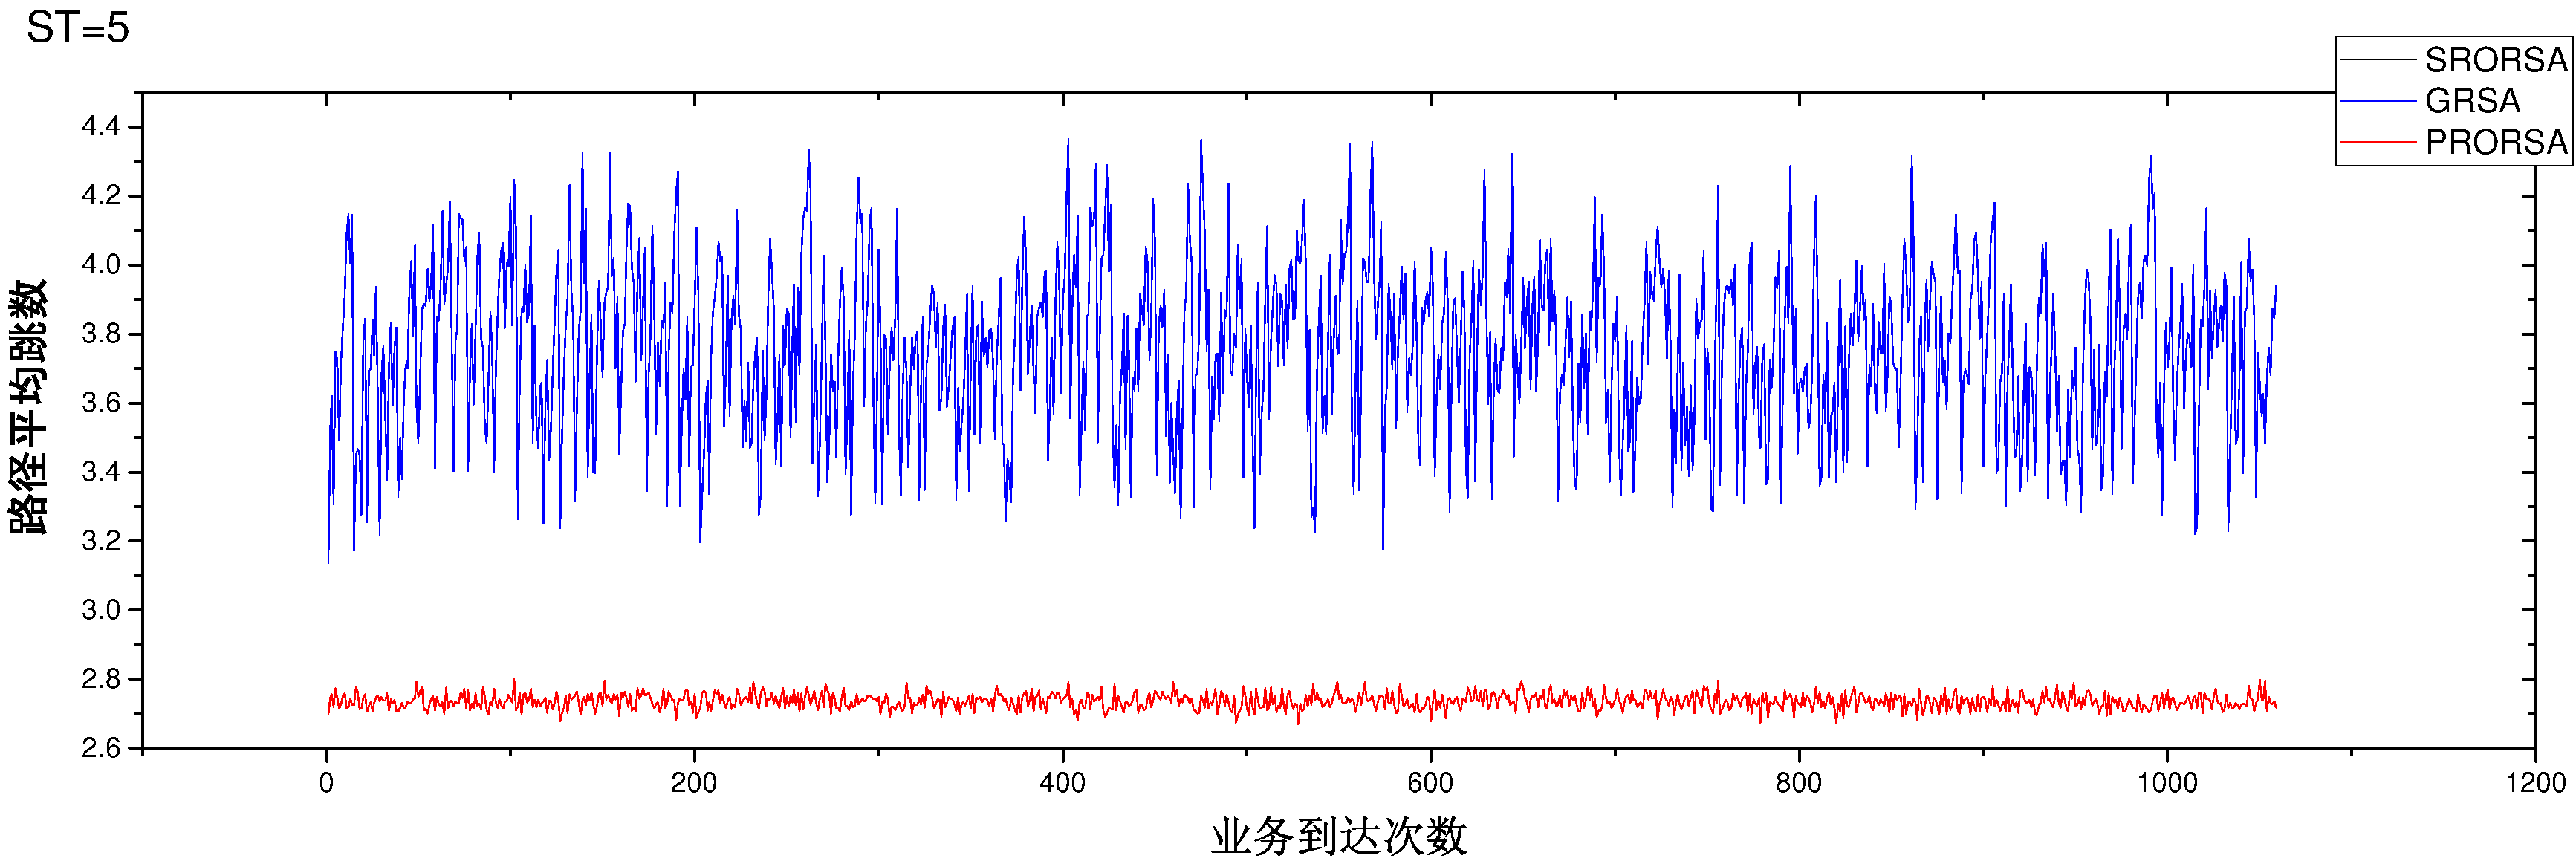
\includegraphics[width=1 \textwidth]{figures/B5H.pdf}}
\end{center}
\caption{{\footnotesize{无权图路径跳数对比(ST=5)}}}
\label{B5H}
\end{figure*}
\begin{figure*}
\setlength{\belowcaptionskip}{-0.5cm}
\begin{center}
{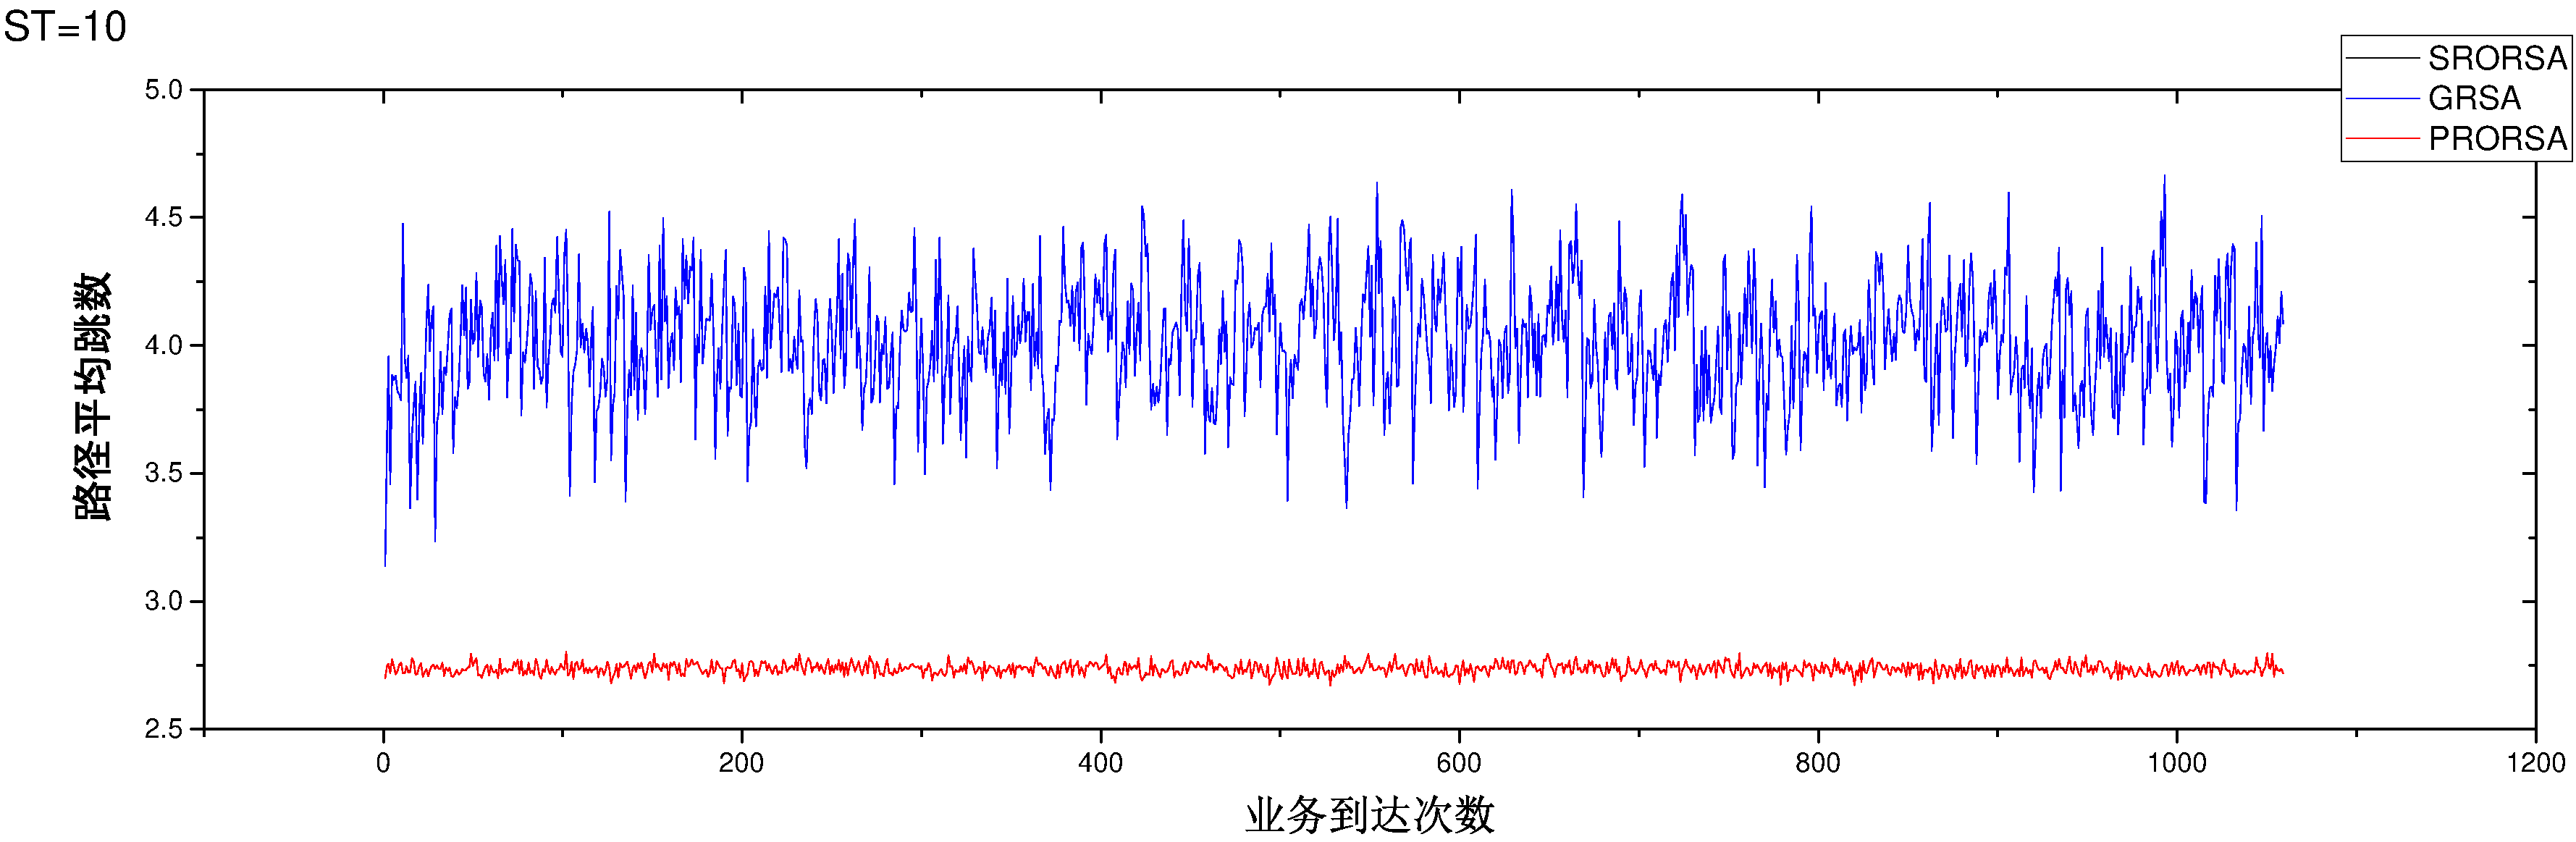
\includegraphics[width=1 \textwidth]{figures/B10H.pdf}}
\end{center}
\caption{{\footnotesize{无权图路径跳数对比(ST=10)}}}
\label{B10H}
\end{figure*}
\begin{figure*}
\setlength{\belowcaptionskip}{-0.5cm}
\begin{center}
{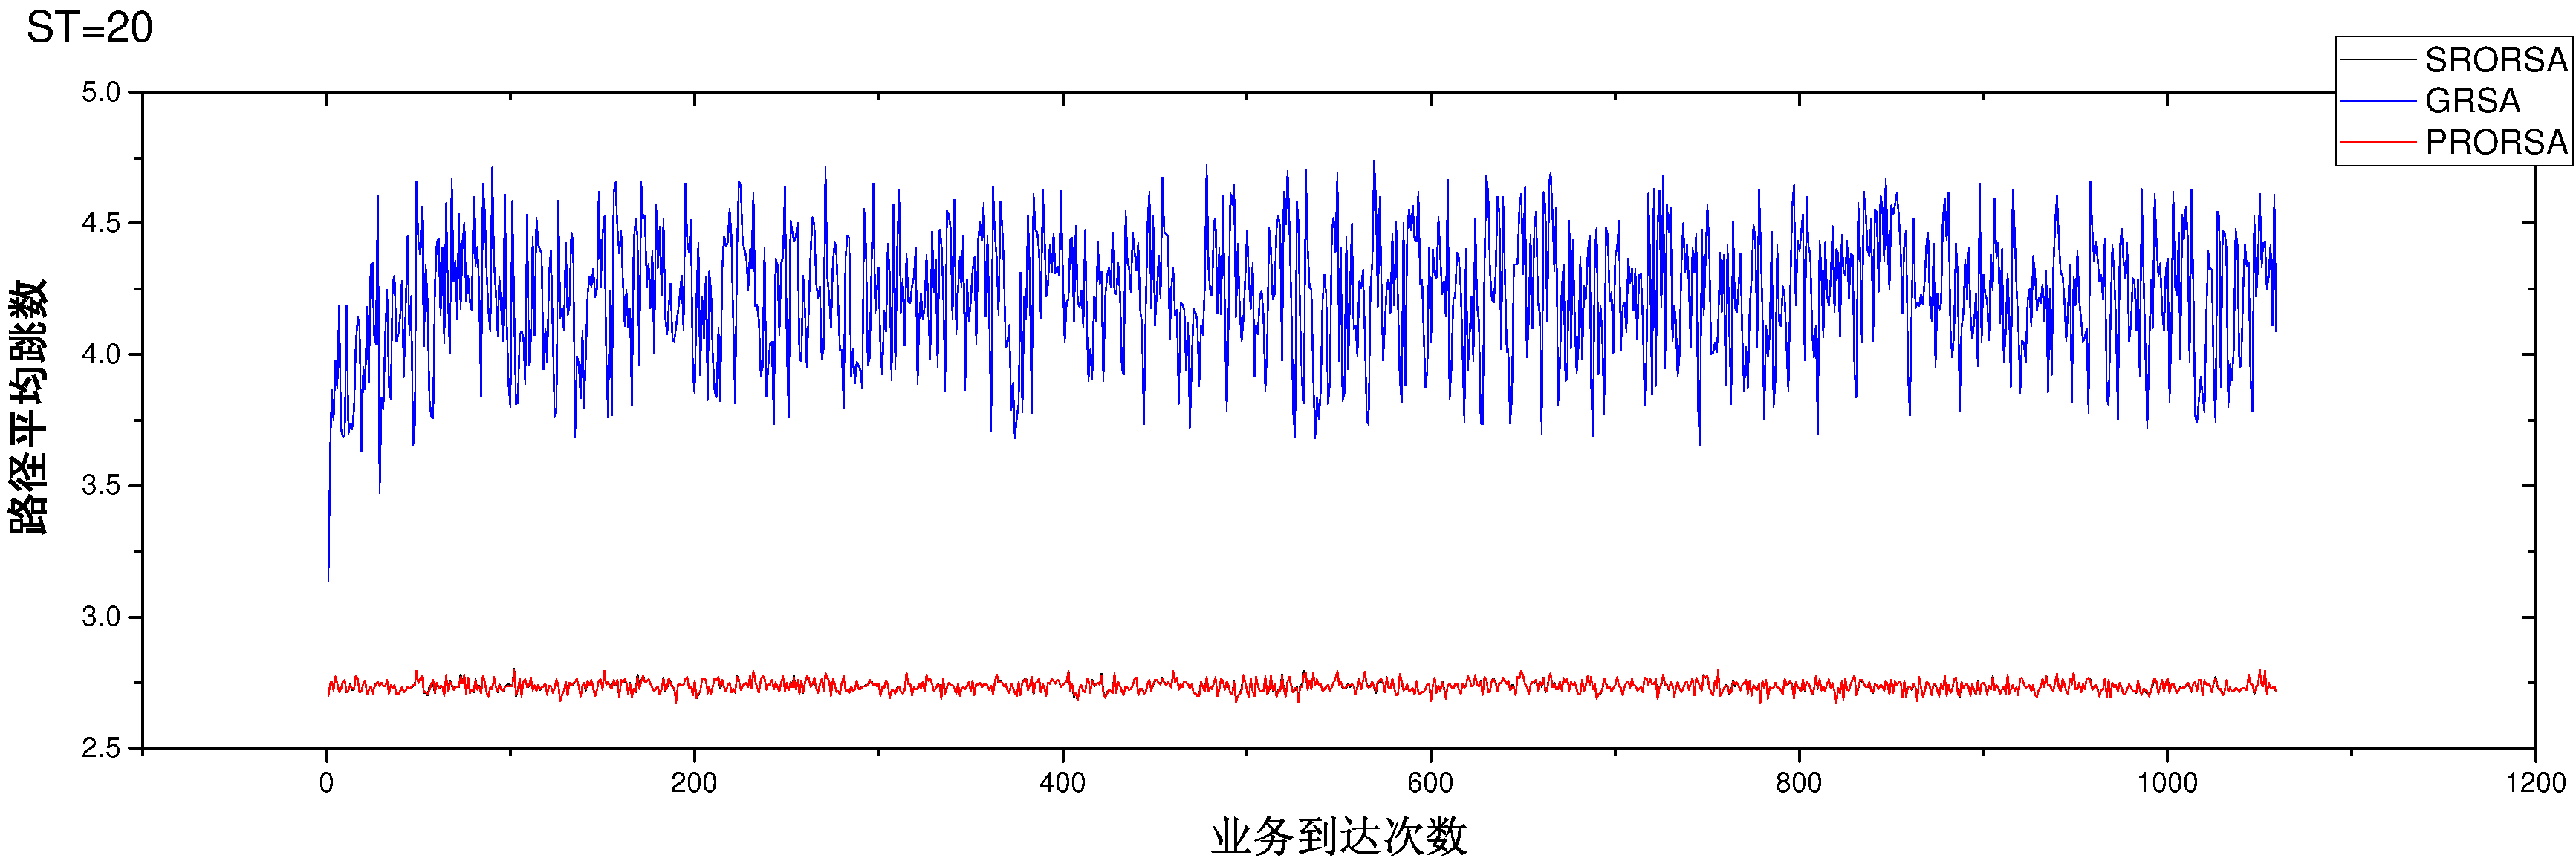
\includegraphics[width=1 \textwidth]{figures/B20H.pdf}}
\end{center}
\caption{{\footnotesize{无权图路径跳数对比(ST=20)}}}
\label{B20H}
\end{figure*}
\begin{figure*}
\setlength{\belowcaptionskip}{-0.5cm}
\begin{center}
{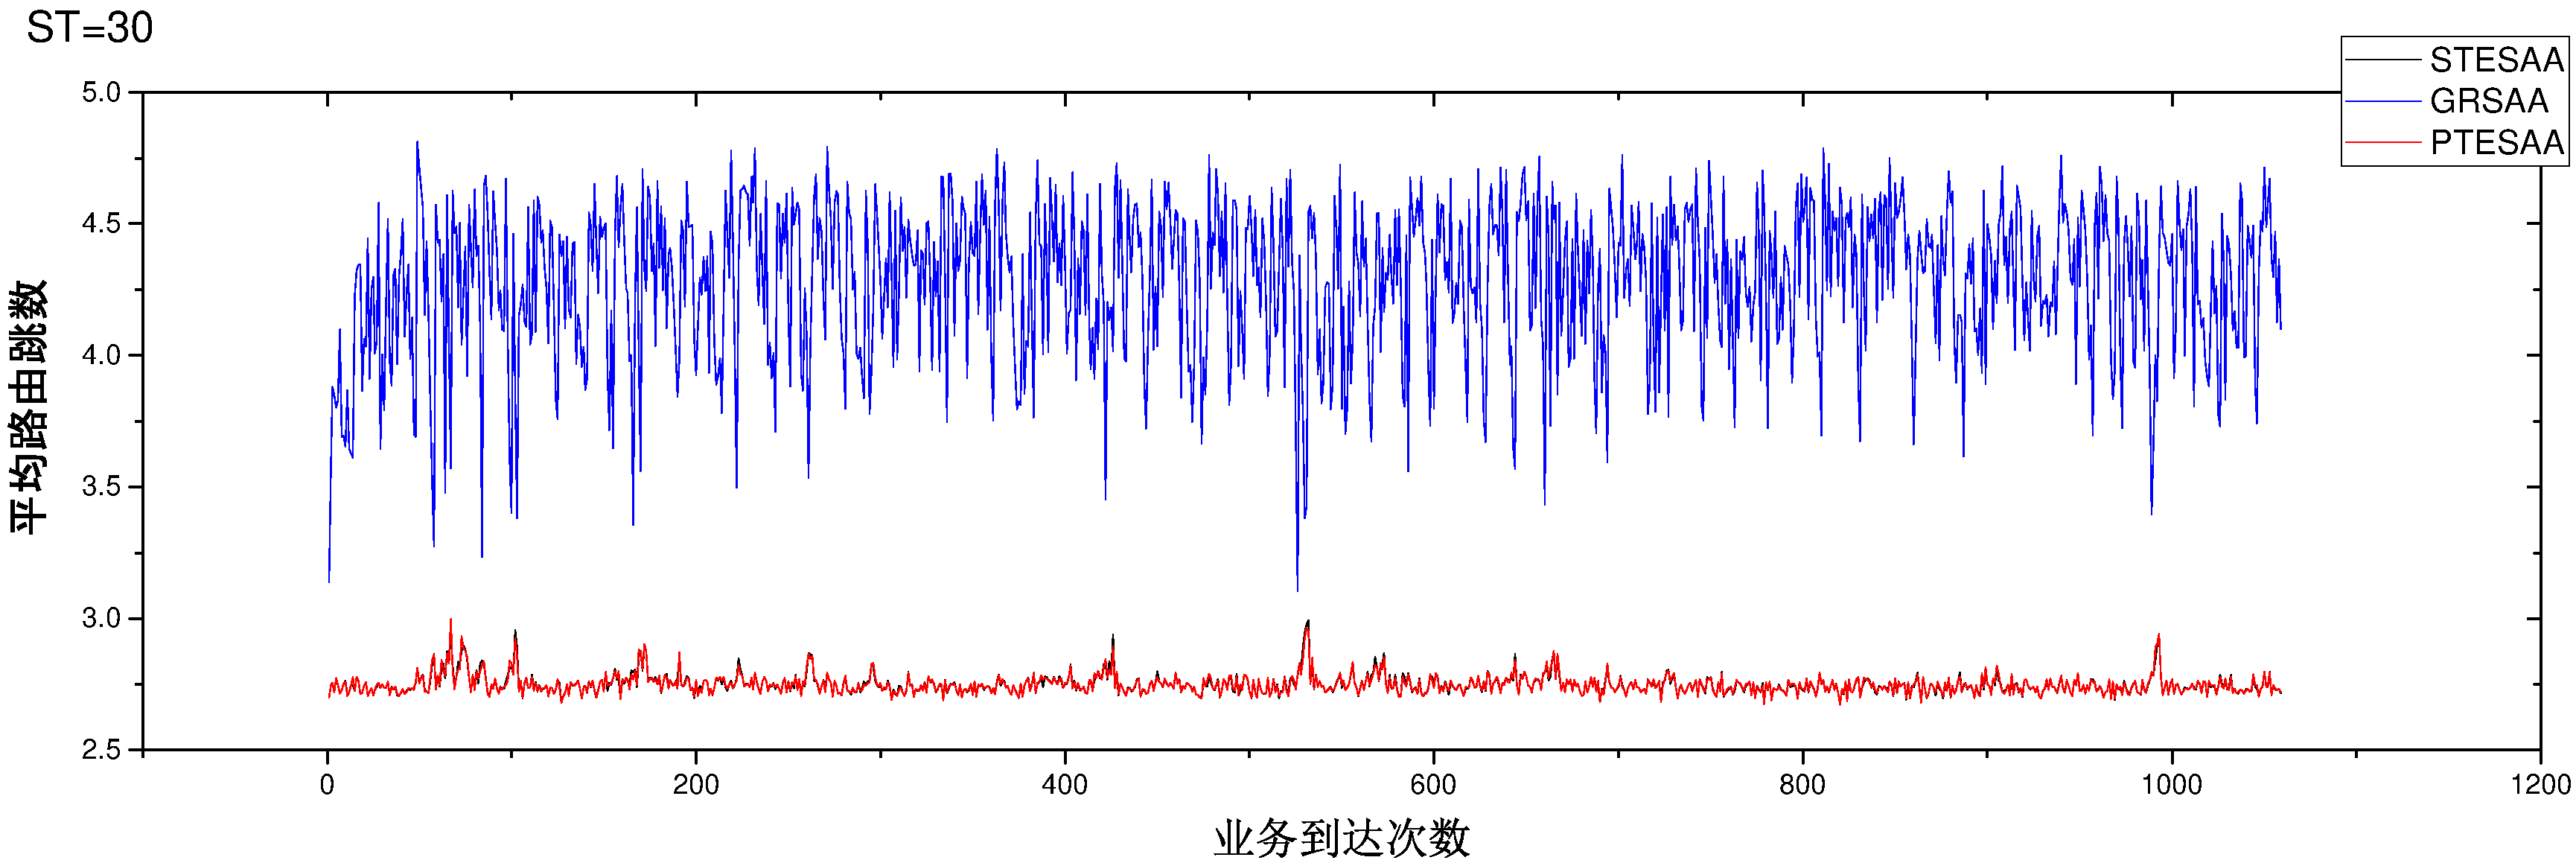
\includegraphics[width=1 \textwidth]{figures/B30H.pdf}}
\end{center}
\caption{{\footnotesize{无权图路径跳数对比(ST=30)}}}
\label{B30H}
\end{figure*}
\begin{figure*}
\setlength{\belowcaptionskip}{-0.5cm}
\begin{center}
{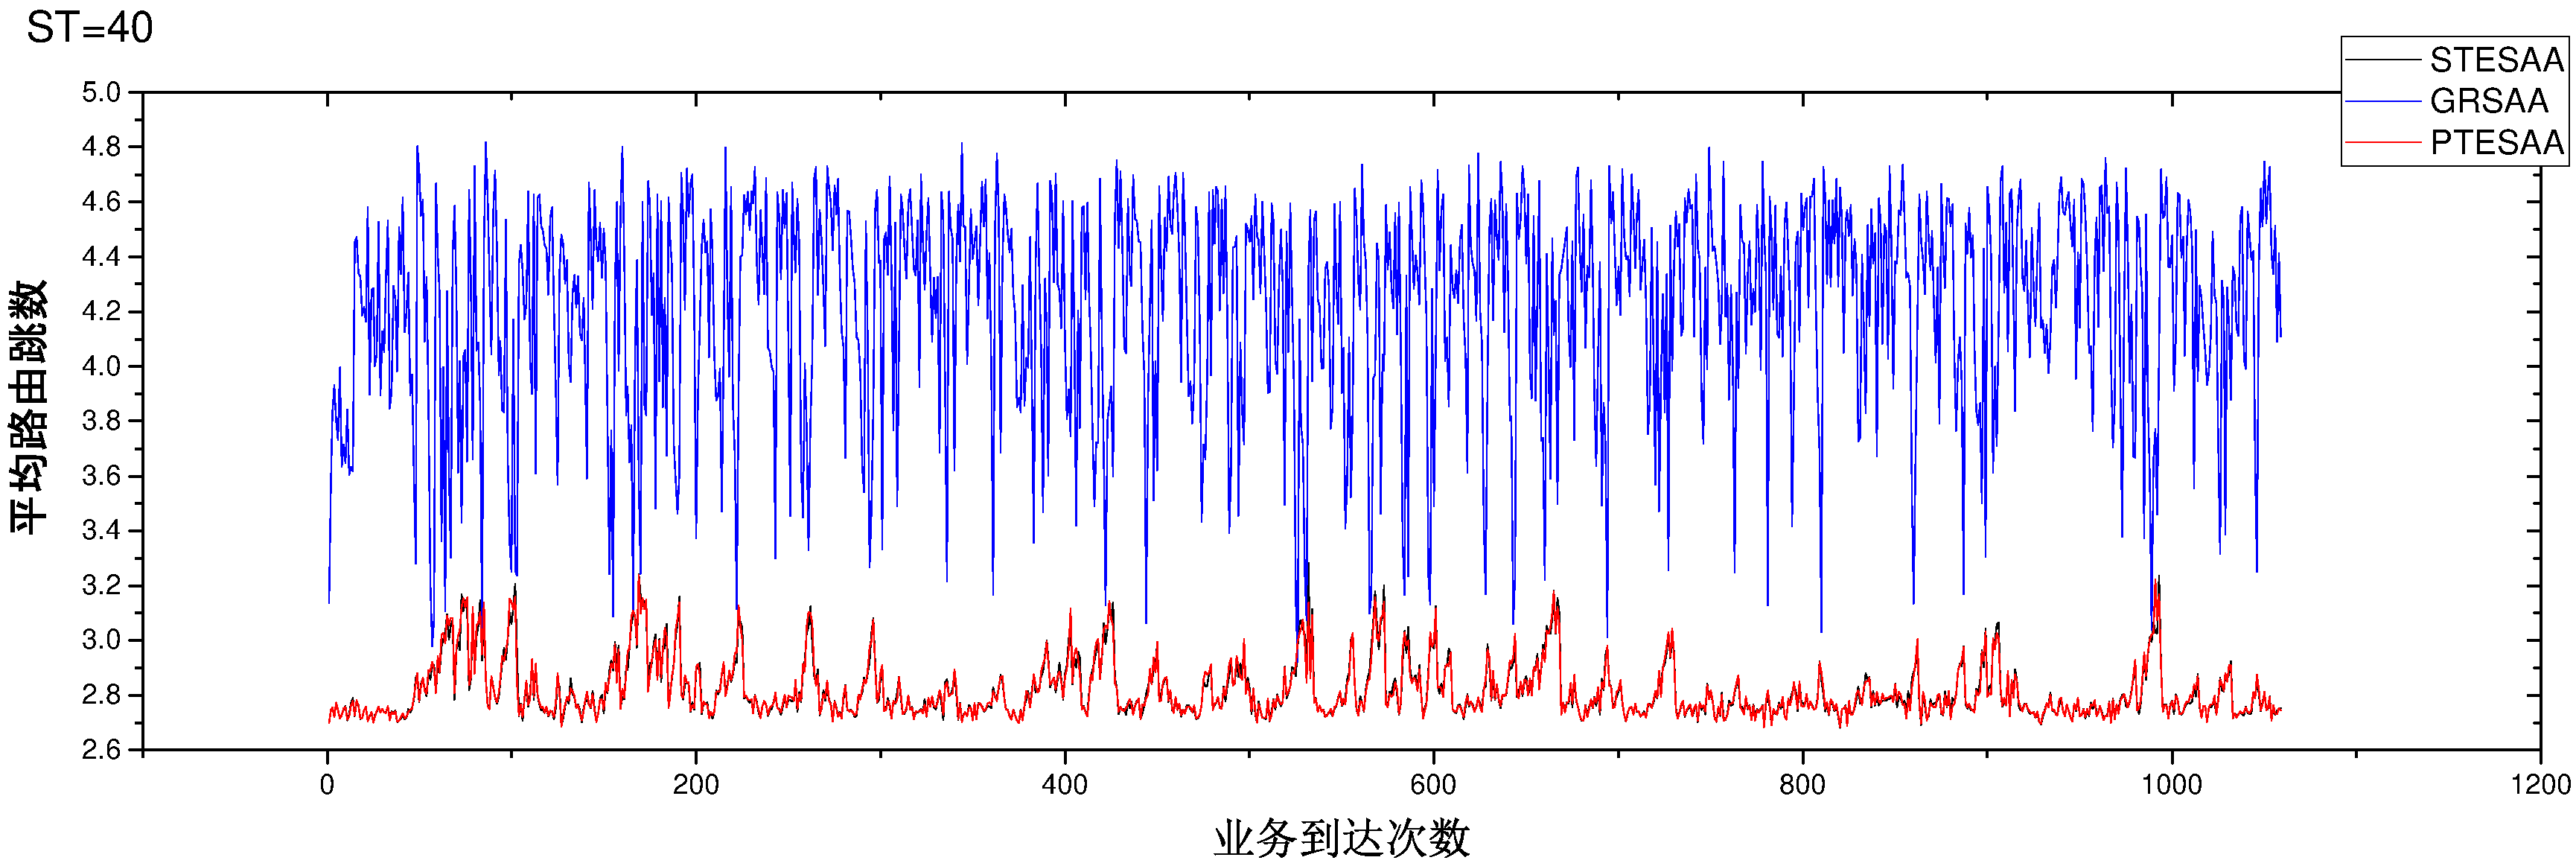
\includegraphics[width=1 \textwidth]{figures/B40H.pdf}}
\end{center}
\caption{{\footnotesize{无权图路径跳数对比(ST=40)}}}
\label{B40H}
\end{figure*}
\subsubsection{时间分析}

图 \ref{B5T}到图 \ref{B40T}展示了在不同平均服务时间$ST$下的各种算法的计算时间,当$ST=5$时,我们可以看到通过GPU加速的PRORSA的计算时间是SPROA 的计算时间的1/4,而实际上备选路径部分的GPU加速达到了7-8 倍,但是由于步骤二的快速路径选择过程也需要消耗一部分时间,这部分时间不能进行GPU加速,实际上PRORSA的大部分算法时间花在了步骤二的路径选择上,所以使得总体的加速比下降为4倍左右。我们发现由于PRORSA的波动幅度比SRORSA的波动幅度小很多,这是因为SRORSA的大部分时间花在计算备选路上,备选路径的计算量随着业务数量和网络链路的占用情况变化较大,而PRORSA的计算量花在步骤二上,计算量变化较小。GRSA的计算时间略高于PRORSA的计算时间,而且GRSA的波动幅度很大,不够平稳,这是因为GRSA贪心策略占用链路资源过多,容易造成分层图链路的碎片化,使得计算量变化较大。
观察到随着$ST$的变化PRORSA的对SRORSA的加速比逐渐下降,这是因为随着网络压力的增加,可用链路变少,使得SRORSA的备选路径计算复杂度下降,PRORSA加速优势变小。另外,随着$ST$的增加,PRORSA 和SRORSA的时间波动幅度增加,这是因为由于链路繁忙,使得大量业务不能一次性加入,步骤二到步骤一之间的循环次数增加,使得某些业务到达点的业务需要多次的循环,计算时间变长,从而拉大了时间变化幅度。
\begin{figure*}
\setlength{\belowcaptionskip}{-0.5cm}
\begin{center}
{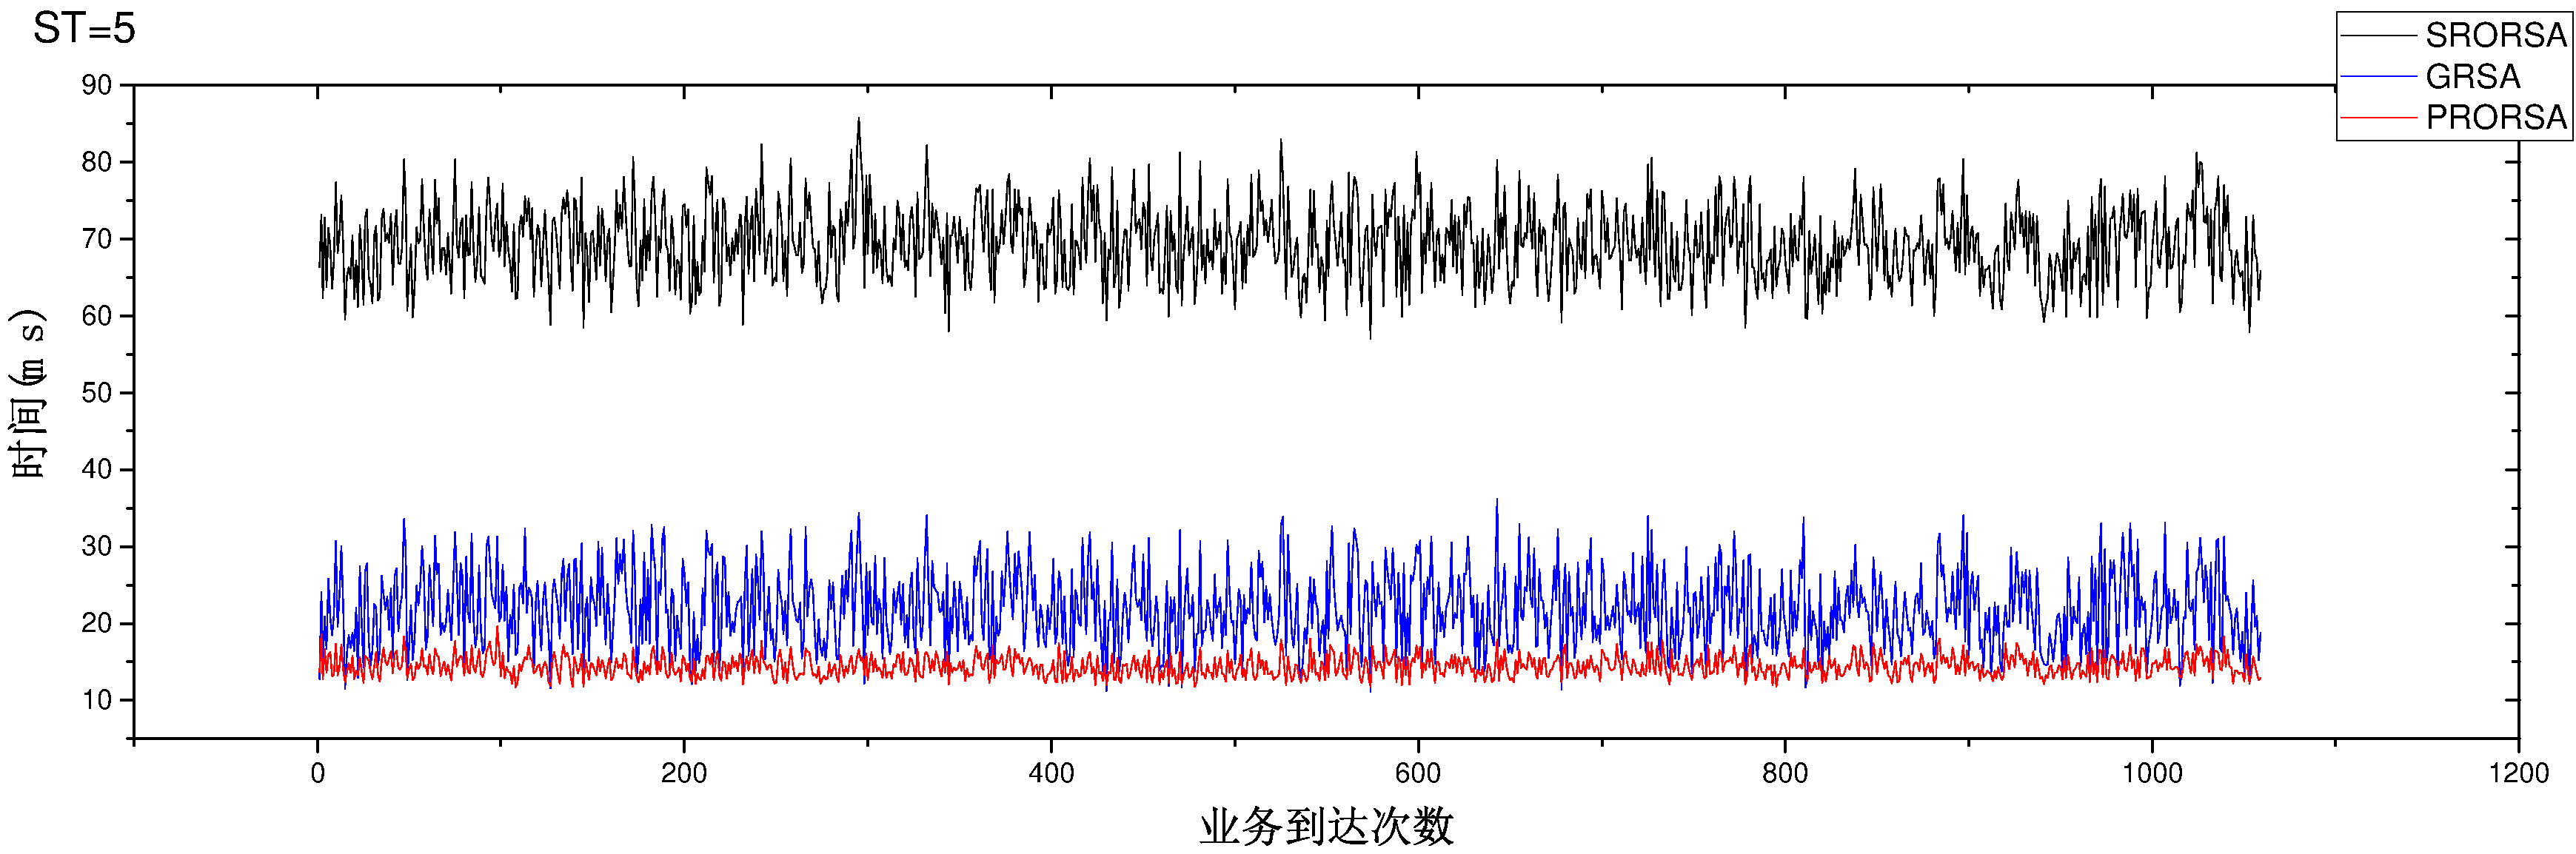
\includegraphics[width=1 \textwidth]{figures/B5T.pdf}}
\end{center}
\caption{{\footnotesize{无权图时间对比(ST=5)}}}
\label{B5T}
\end{figure*}
\begin{figure*}
\setlength{\belowcaptionskip}{-0.5cm}
\begin{center}
{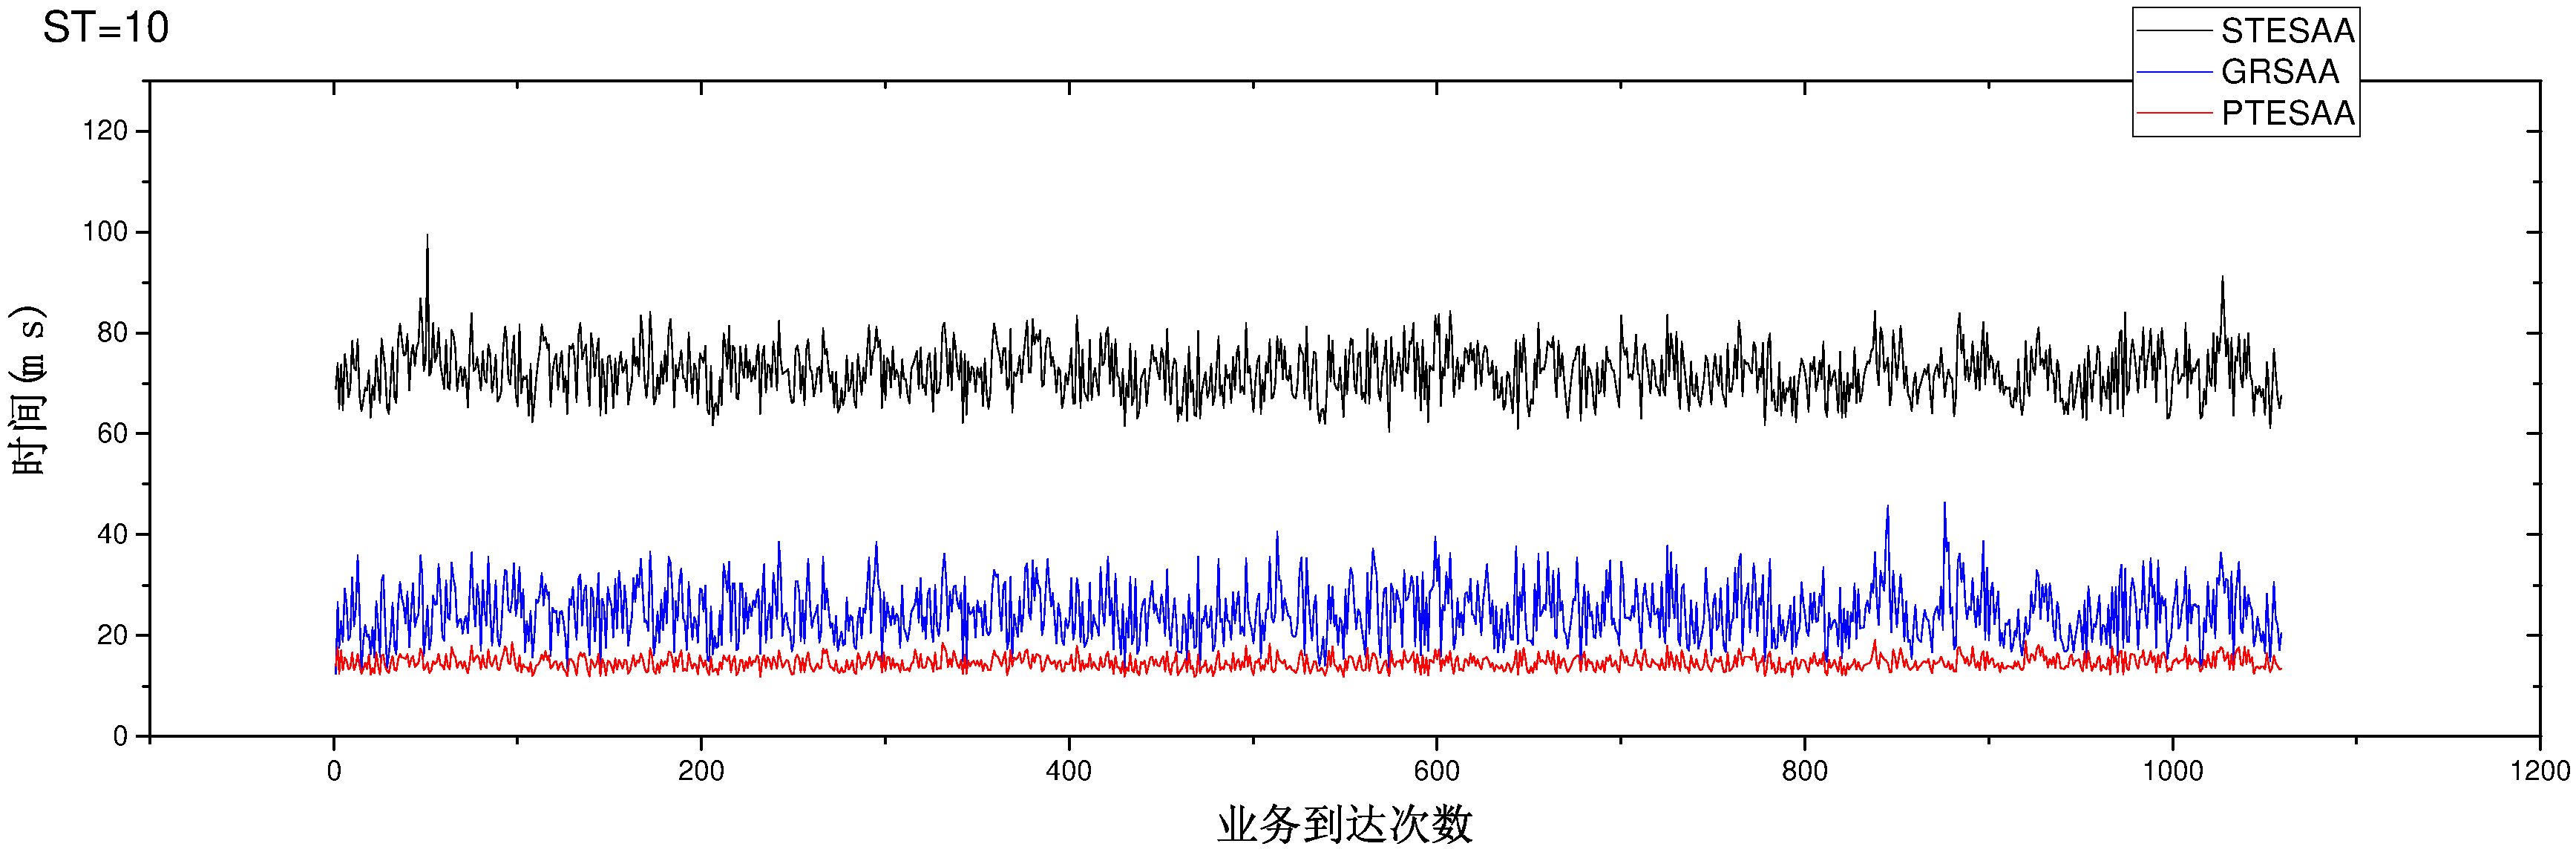
\includegraphics[width=1 \textwidth]{figures/B10T.pdf}}
\end{center}
\caption{{\footnotesize{无权图时间对比(ST=10)}}}
\label{B10T}
\end{figure*}
\begin{figure*}
\setlength{\belowcaptionskip}{-0.5cm}
\begin{center}
{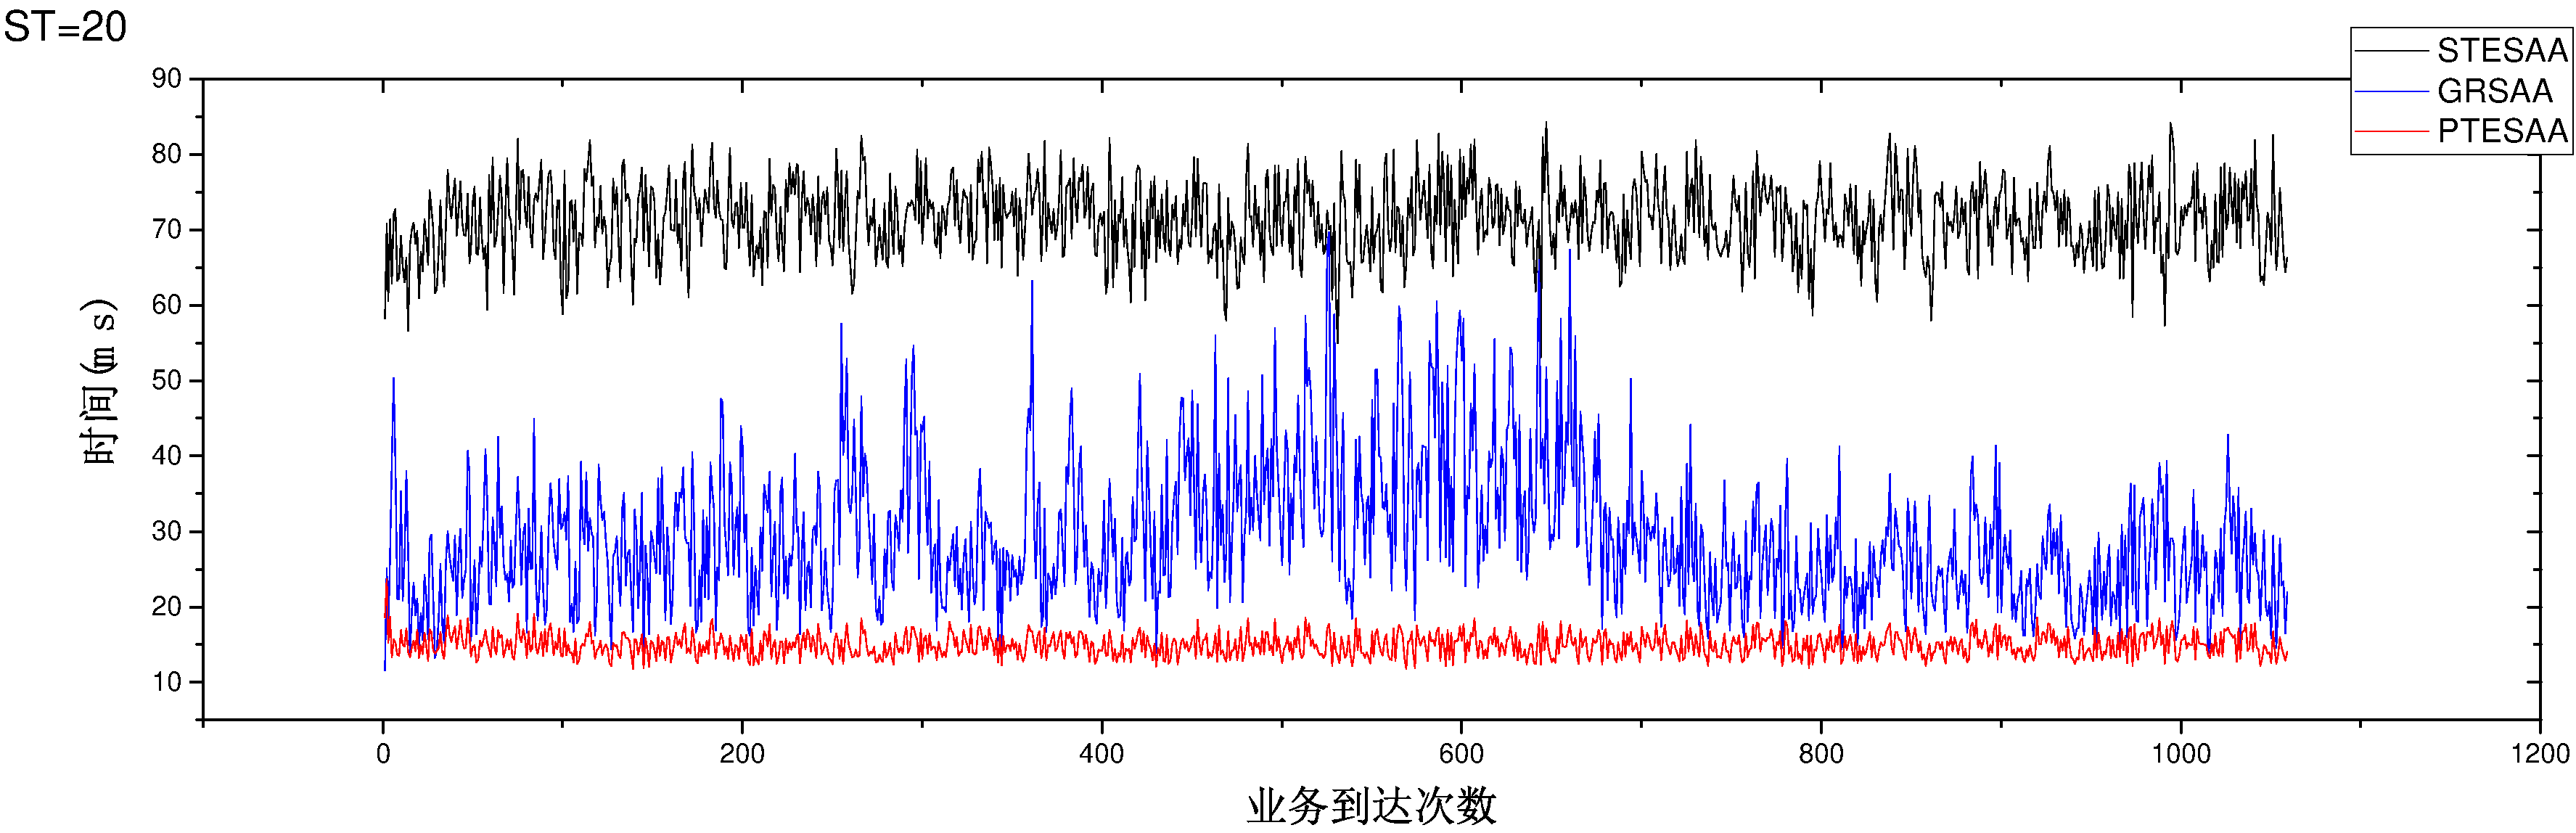
\includegraphics[width=1 \textwidth]{figures/B20T.pdf}}
\end{center}
\caption{{\footnotesize{无权图时间对比(ST=20)}}}
\label{B20T}
\end{figure*}
\begin{figure*}
\setlength{\belowcaptionskip}{-0.5cm}
\begin{center}
{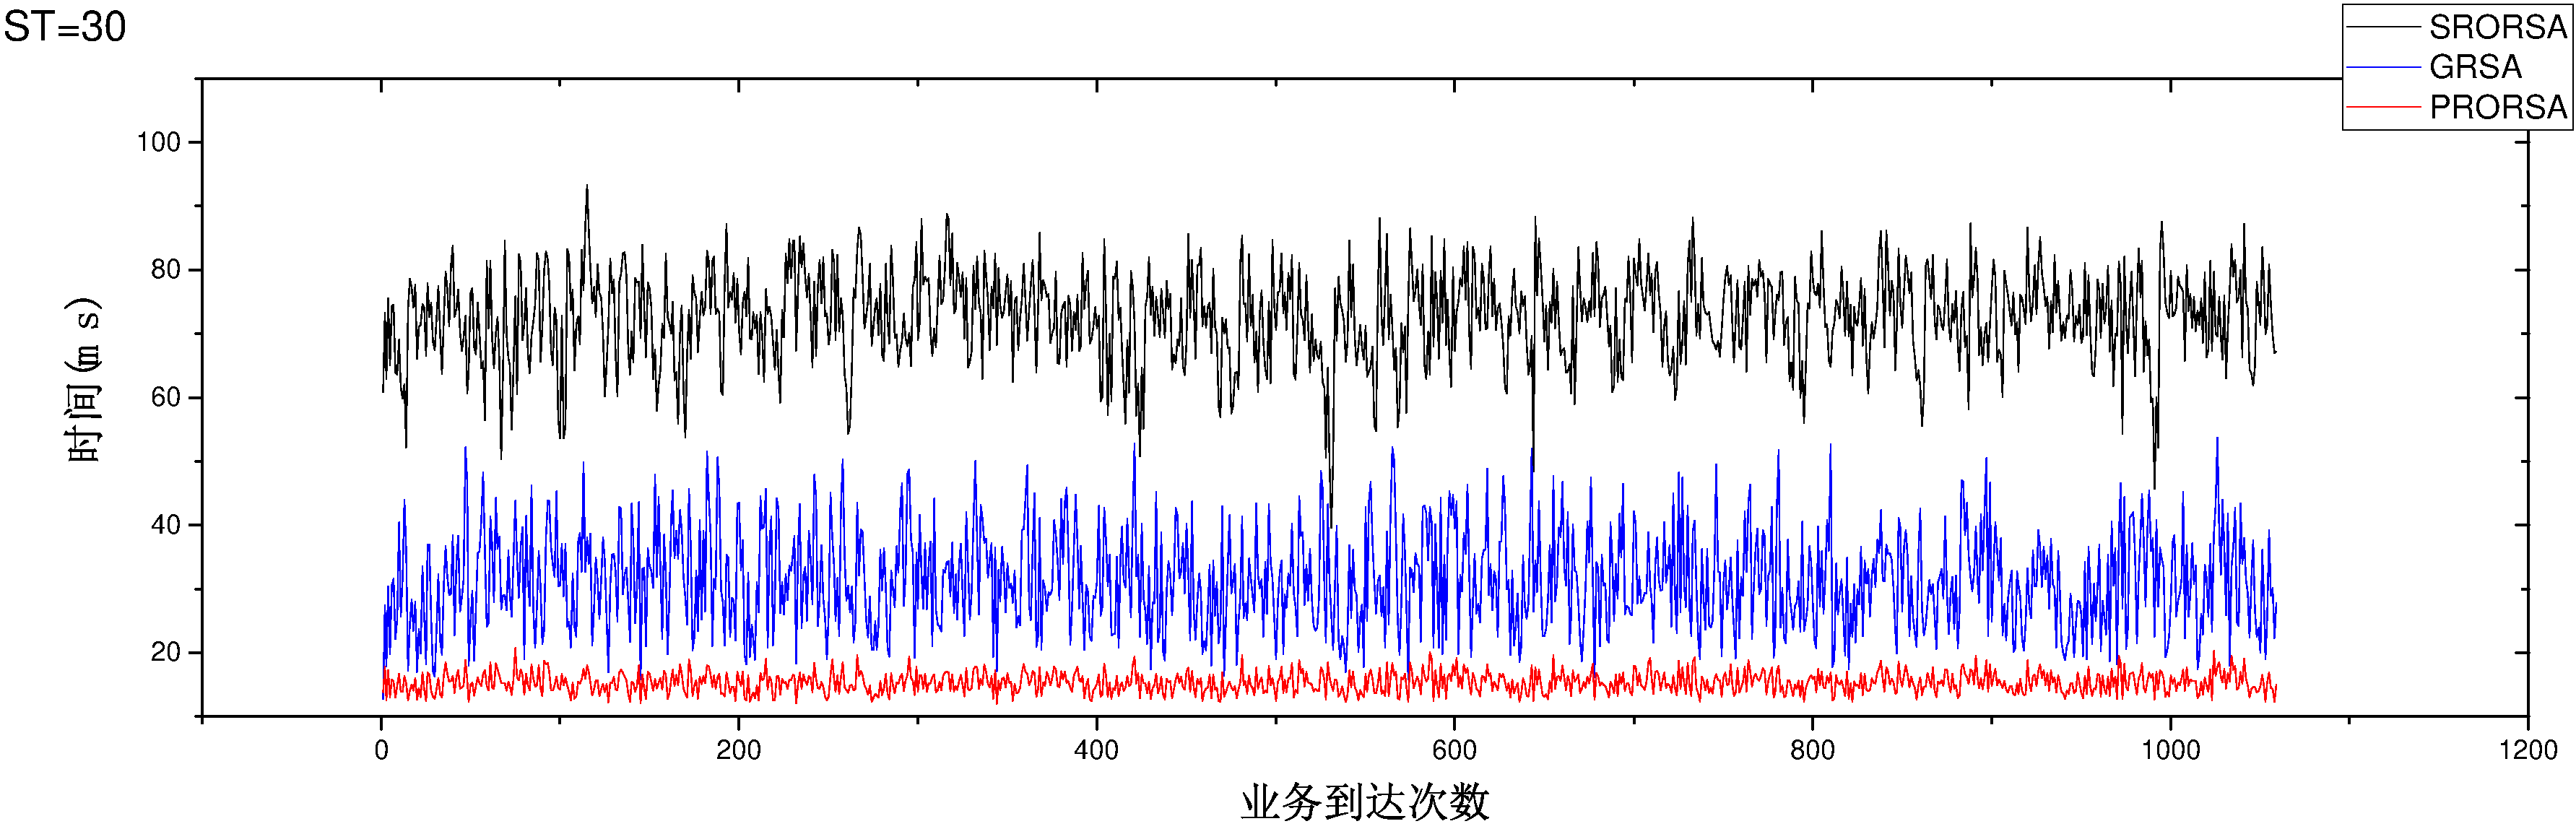
\includegraphics[width=1 \textwidth]{figures/B30T.pdf}}
\end{center}
\caption{{\footnotesize{无权图时间对比(ST=30)}}}
\label{B30T}
\end{figure*}
\begin{figure*}
\setlength{\belowcaptionskip}{-0.5cm}
\begin{center}
{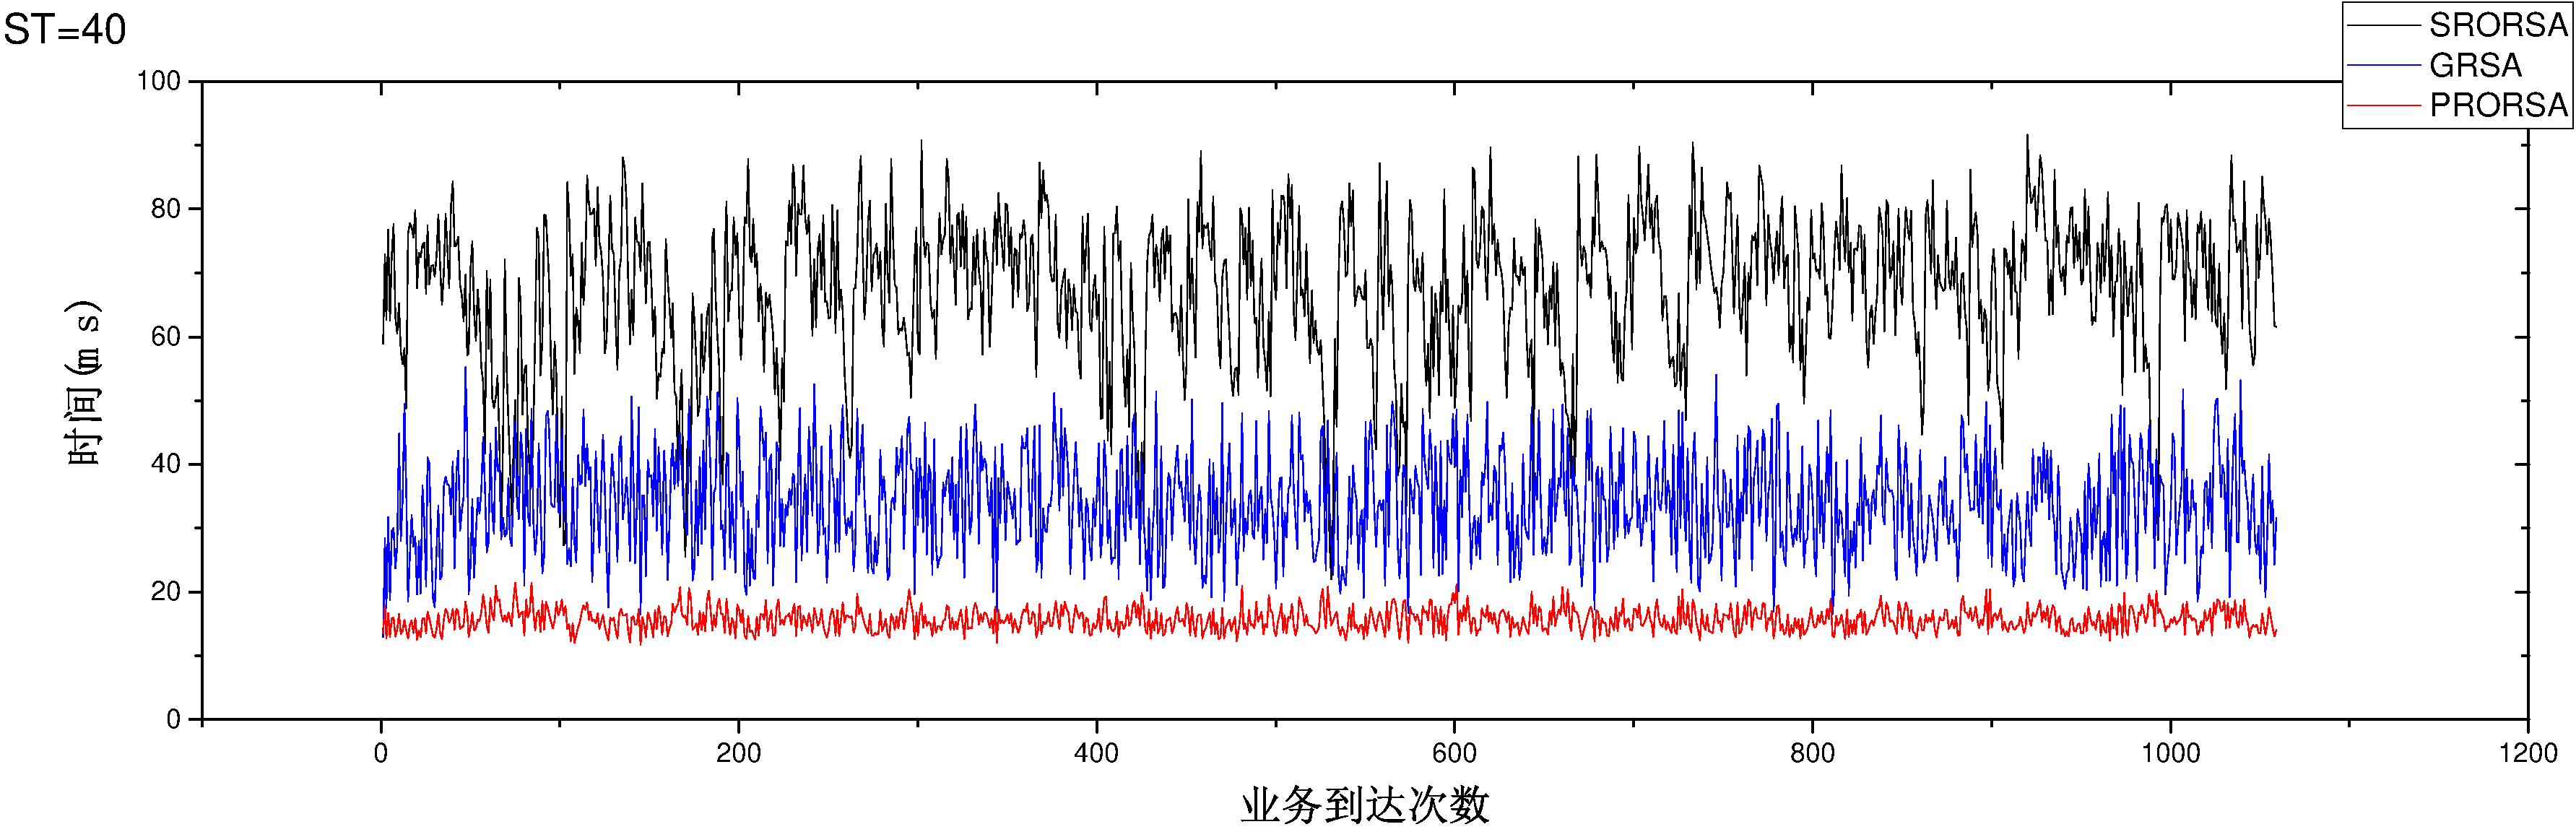
\includegraphics[width=1 \textwidth]{figures/B40T.pdf}}
\end{center}
\caption{{\footnotesize{无权图时间对比(ST=40)}}}
\label{B40T}
\end{figure*}
\subsubsection{阻塞率分析}

图 \ref{B10Z}到图 \ref{B40Z}展示了随着$ST$的变化,PRORSA,SRORSA和GRSA的阻塞率变化情况,其中PRORSA,SRORSA由于是同一种算法,所以其阻塞率几乎一样。当$ST=10$时,我们发现PRORSA/SRORSA的阻塞次数明显小于GRSA。 当$ST=20$时,PRORSA/SRORSA的阻塞次数和阻塞幅度均小于GRSA,在GRSA中出现了一次相对较大的阻塞,但是PRORSA/SRORSA 中没有出现这种不平稳的阻塞率突变。当$ST=30$时,我们发现PRORSA/SRORSA的阻塞次数和阻塞幅度比GRSA小很多,GRSA的平均阻塞率是PRORSA/SRORSA的6倍左右。当$ST=40$时,PRORSA,SRORSA和GRSA的阻塞率都增加很多,但是PRORSA/SRORSA的阻塞情况还是大大优于GRSA,可见在大服务压力的网络中,PRORSA/SRORSA依然能够有效的减小阻塞率。
\begin{figure*}
\setlength{\belowcaptionskip}{-0.5cm}
\begin{center}
{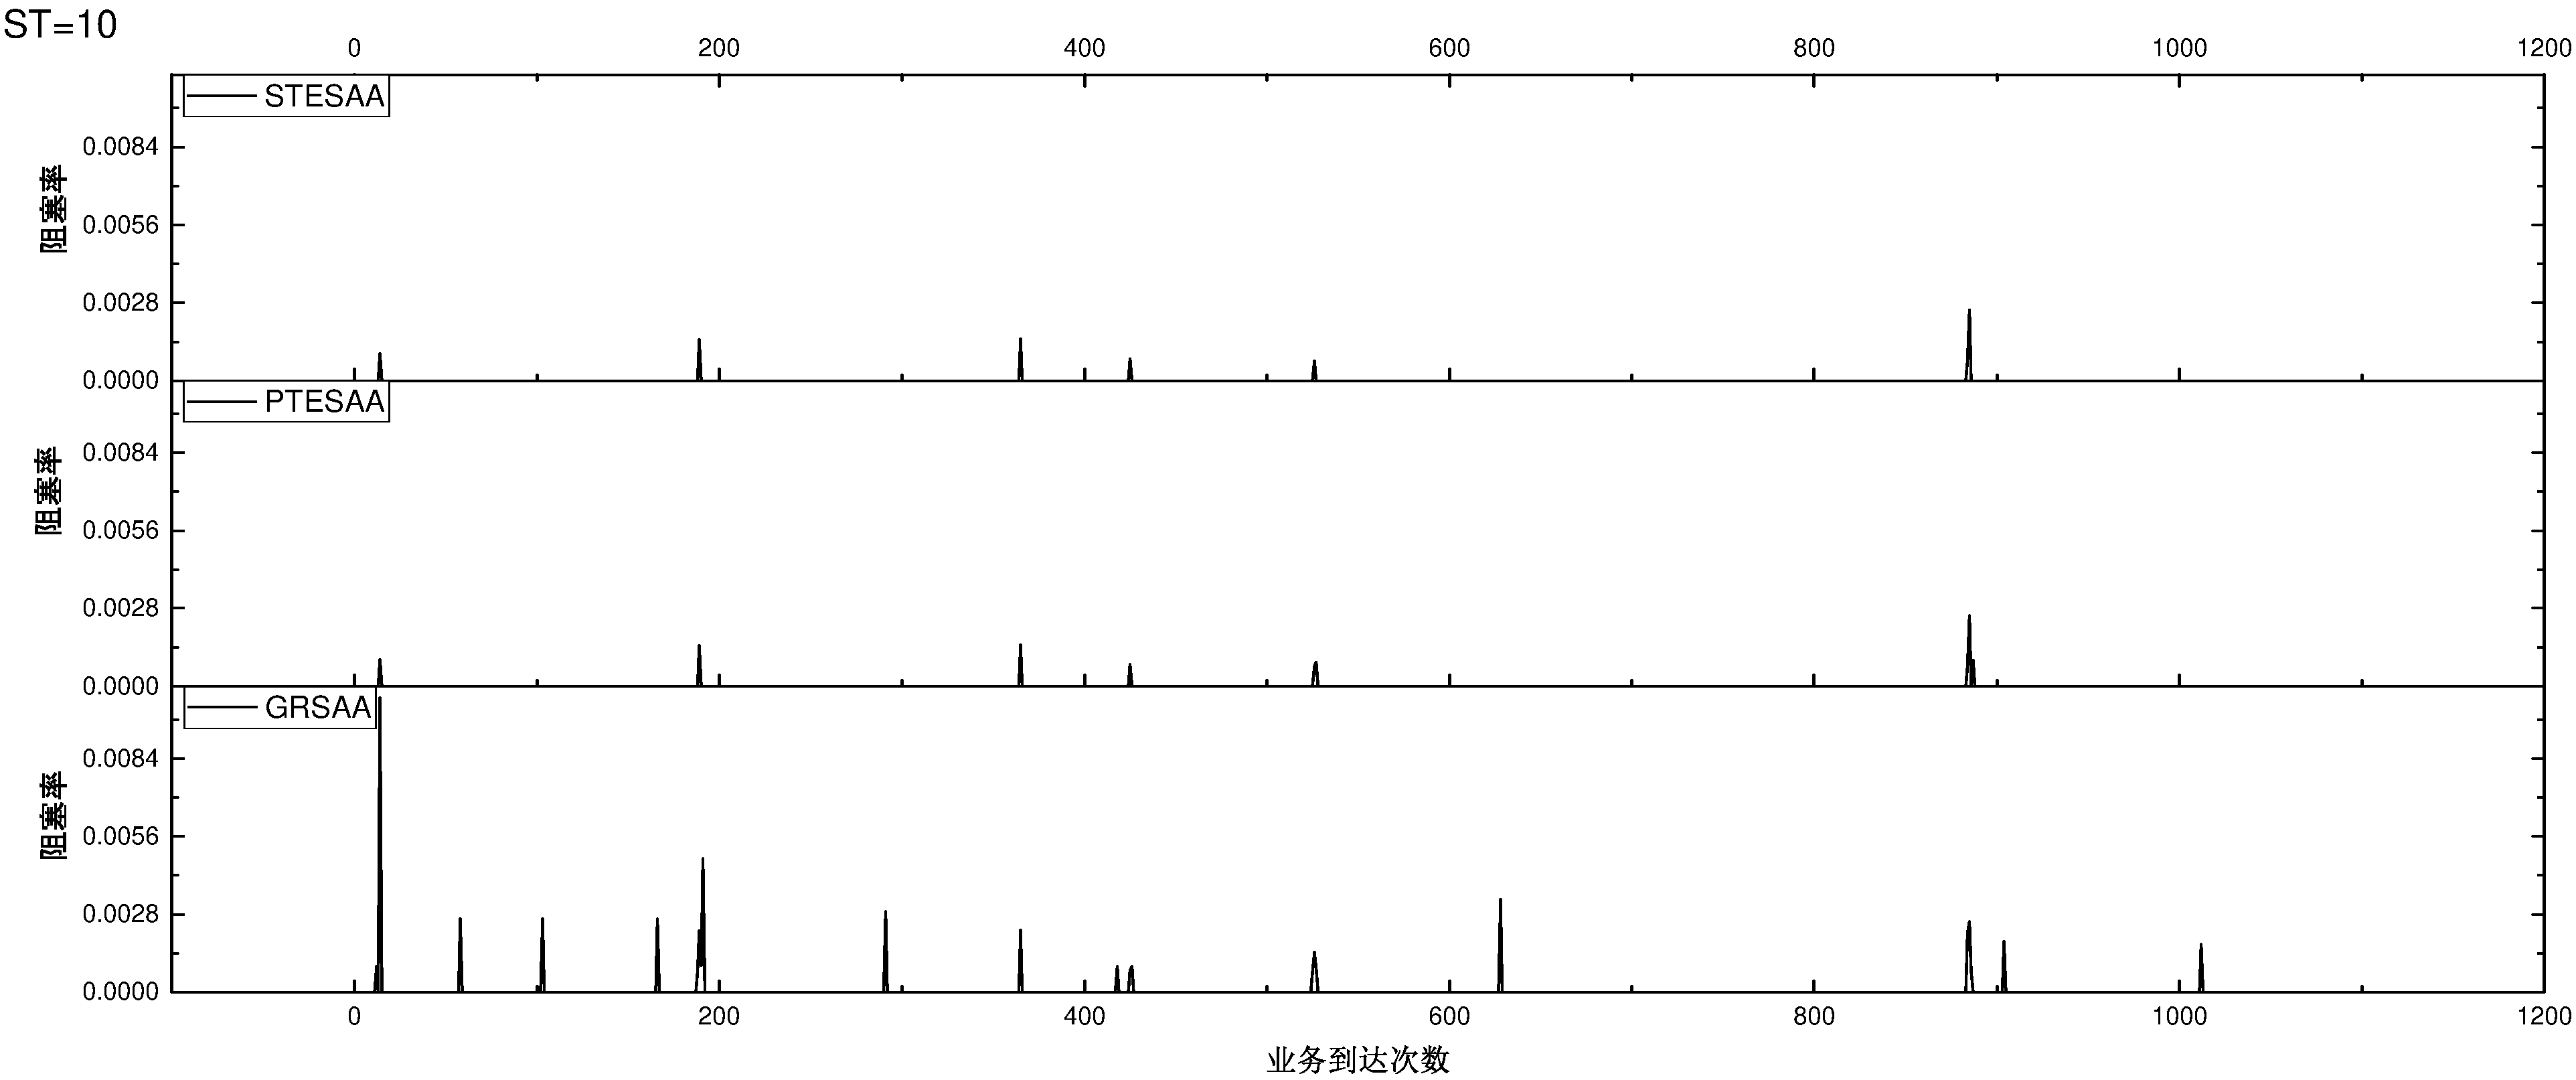
\includegraphics[width=1 \textwidth]{figures/B10Z.pdf}}
\end{center}
\caption{{\footnotesize{无权图阻塞率对比(ST=10)}}}
\label{B10Z}
\end{figure*}
\begin{figure*}
\setlength{\belowcaptionskip}{-0.5cm}
\begin{center}
{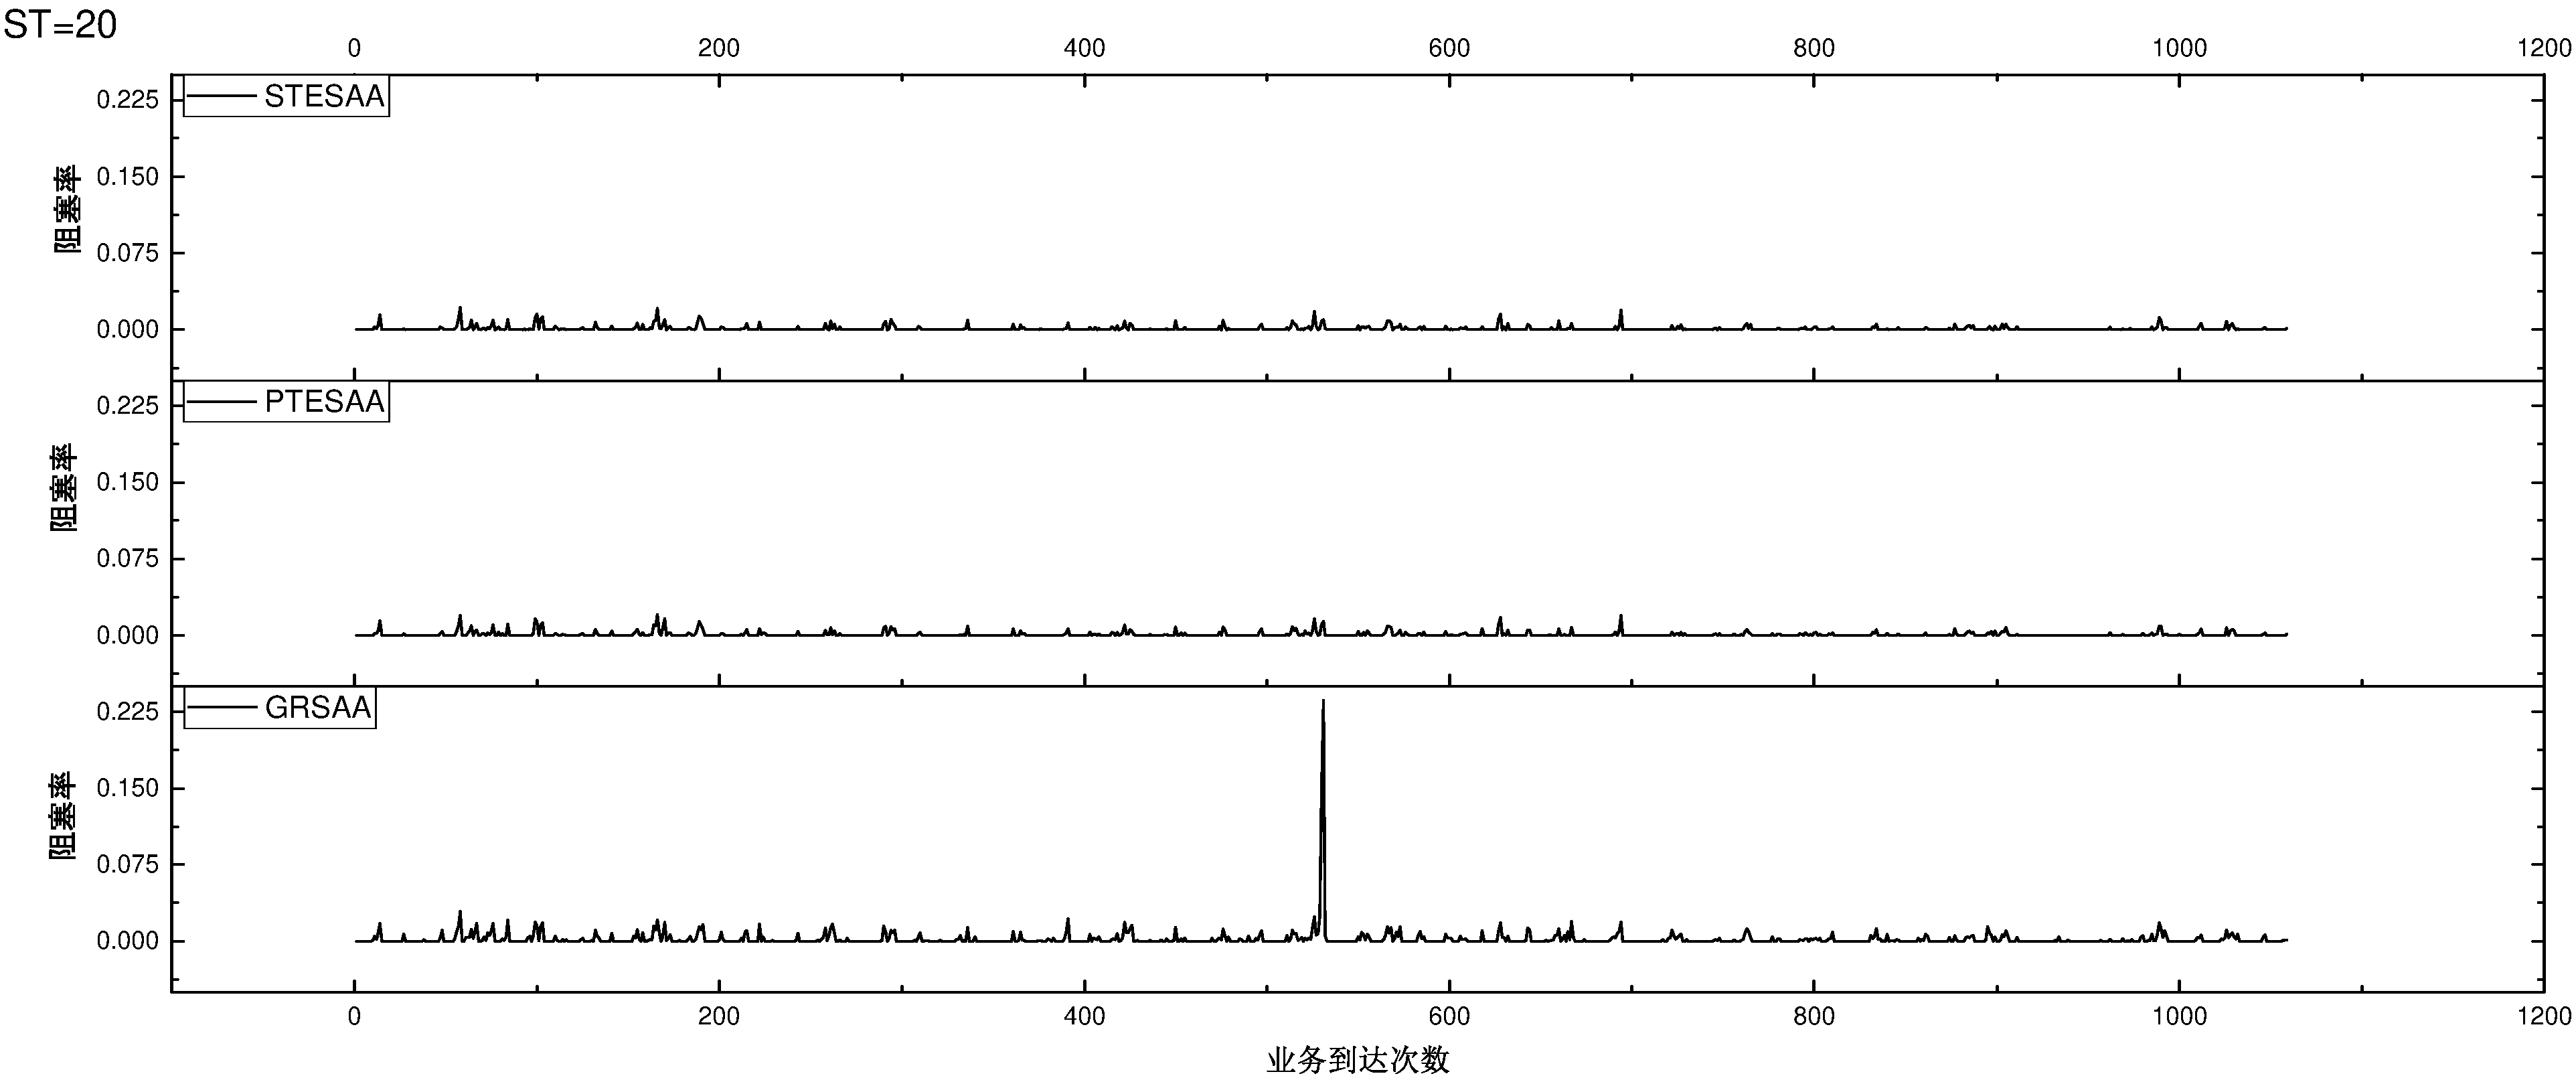
\includegraphics[width=1 \textwidth]{figures/B20Z.pdf}}
\end{center}
\caption{{\footnotesize{无权图阻塞率对比(ST=20)}}}
\label{B20Z}
\end{figure*}
\begin{figure*}
\setlength{\belowcaptionskip}{-0.5cm}
\begin{center}
{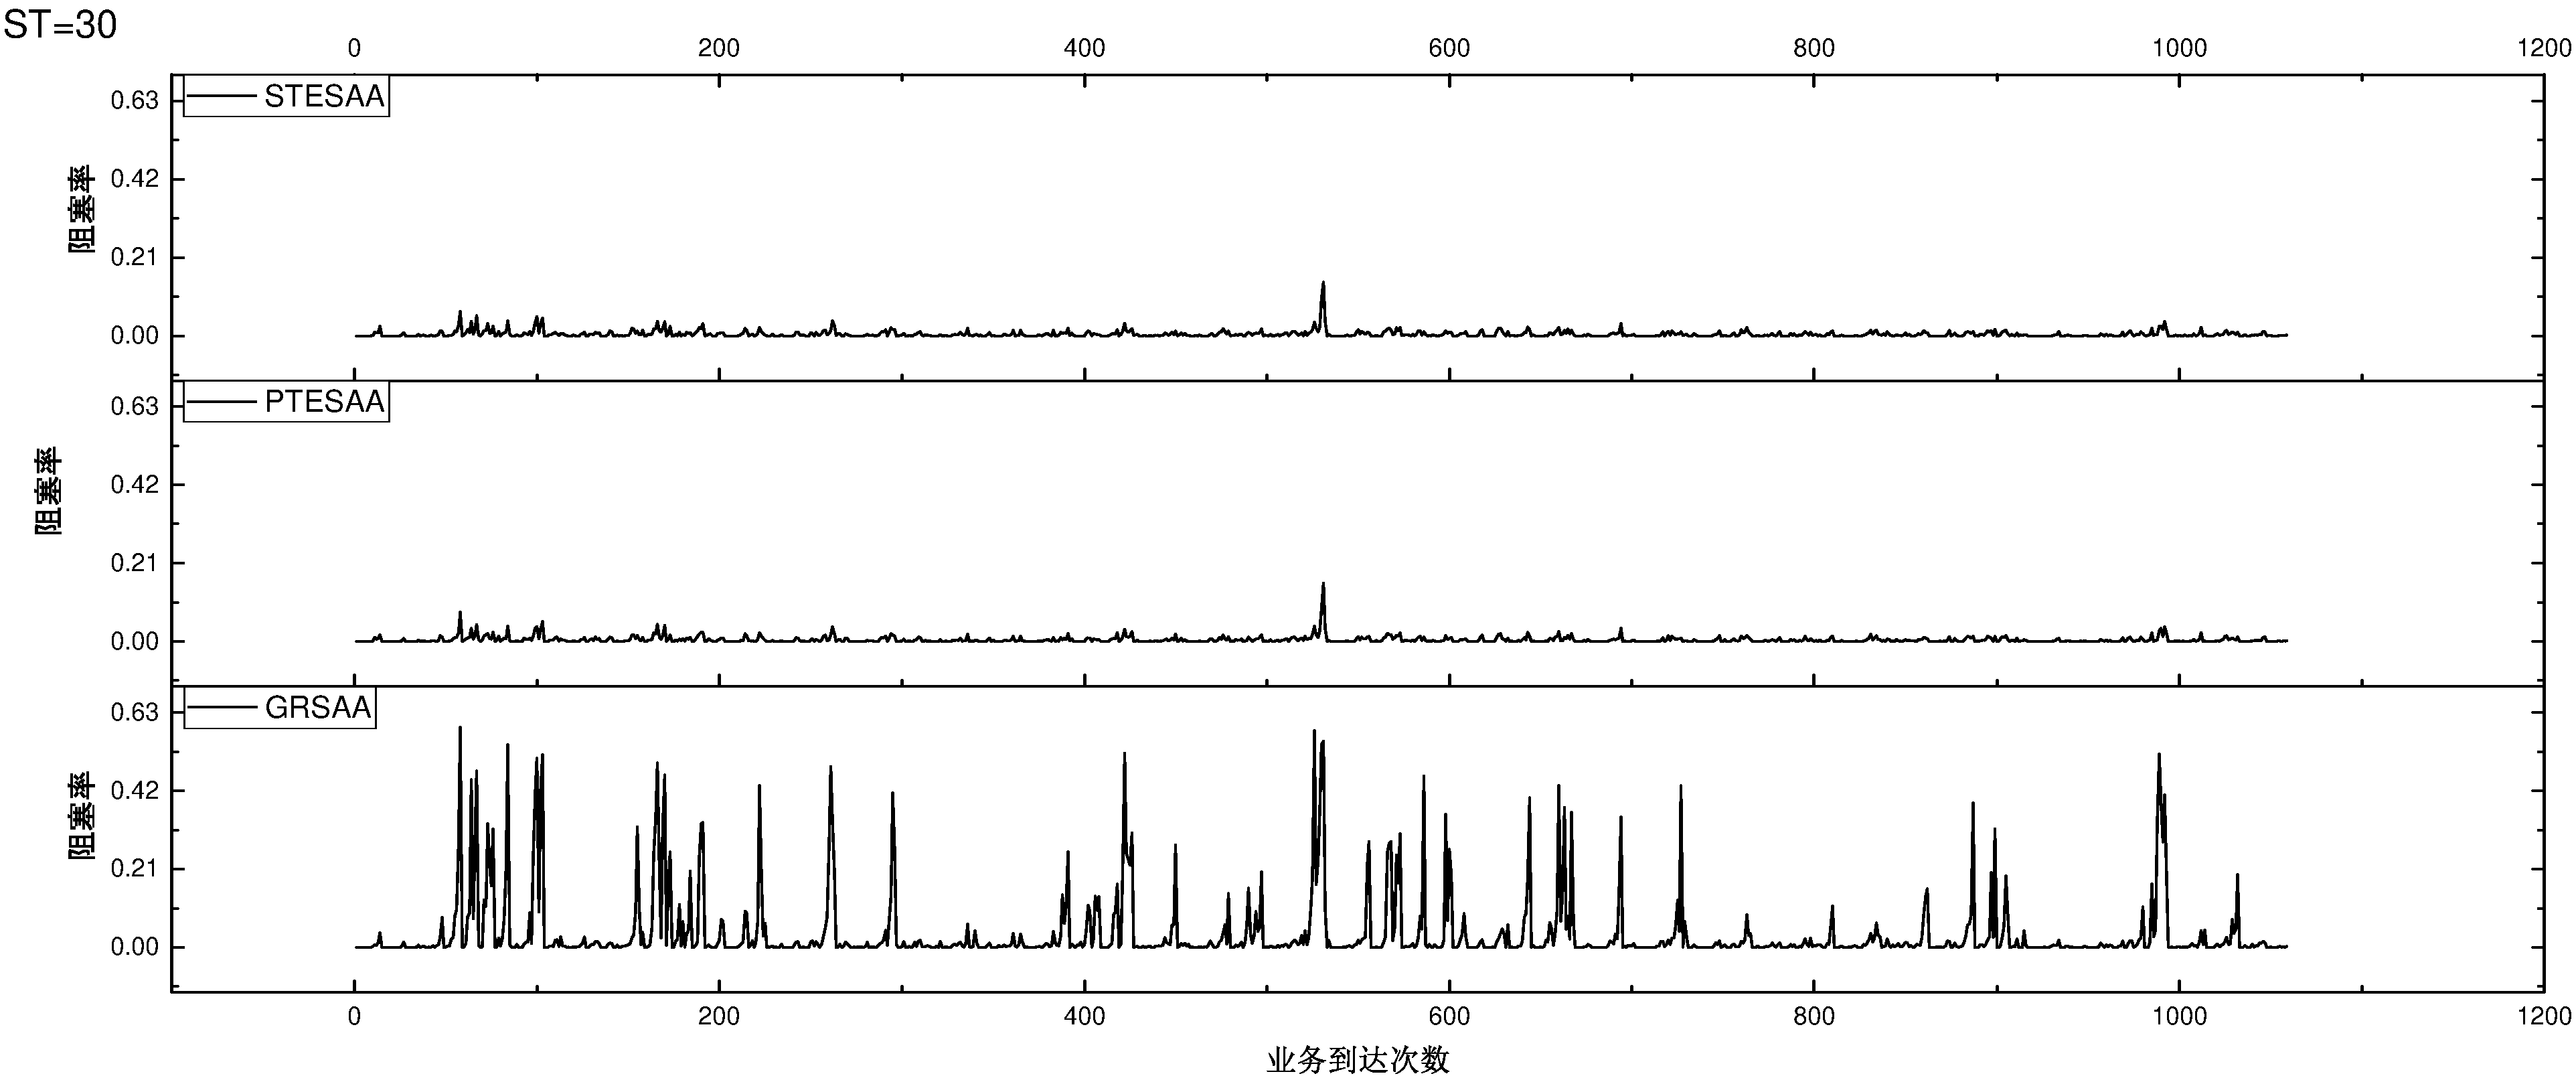
\includegraphics[width=1 \textwidth]{figures/B30Z.pdf}}
\end{center}
\caption{{\footnotesize{无权图阻塞率对比(ST=30)}}}
\label{B30Z}
\end{figure*}
\begin{figure*}
\setlength{\belowcaptionskip}{-0.5cm}
\begin{center}
{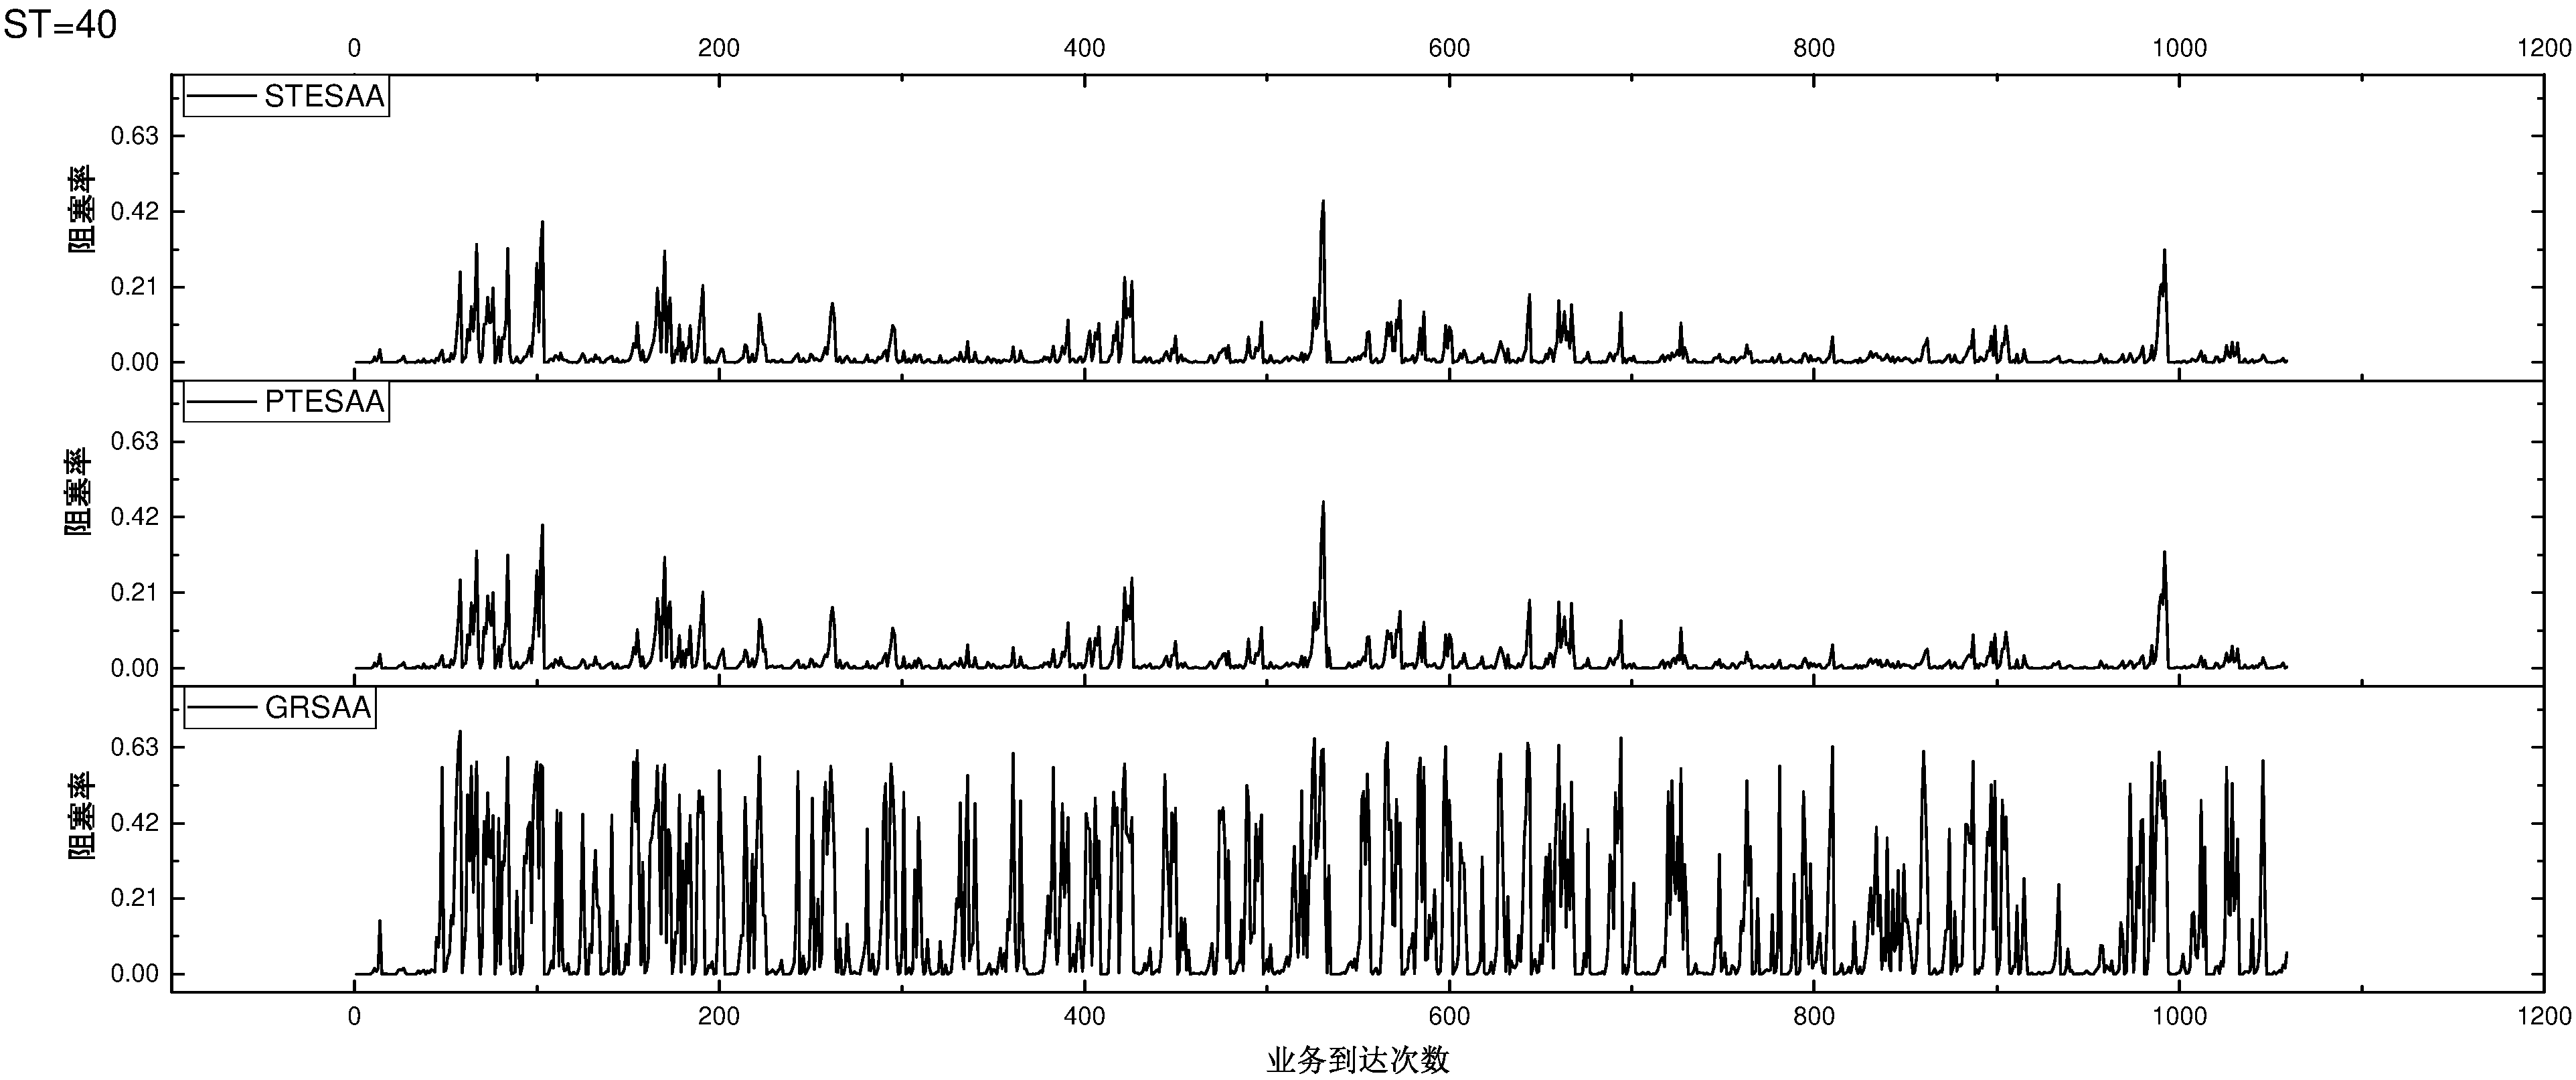
\includegraphics[width=1 \textwidth]{figures/B40Z.pdf}}
\end{center}
\caption{{\footnotesize{无权图阻塞率对比(ST=40)}}}
\label{B40Z}
\end{figure*}
\subsection{带权图下的仿真结果}
\subsubsection{路径优化分析}
\begin{figure*}
\setlength{\belowcaptionskip}{-0.5cm}
\begin{center}
{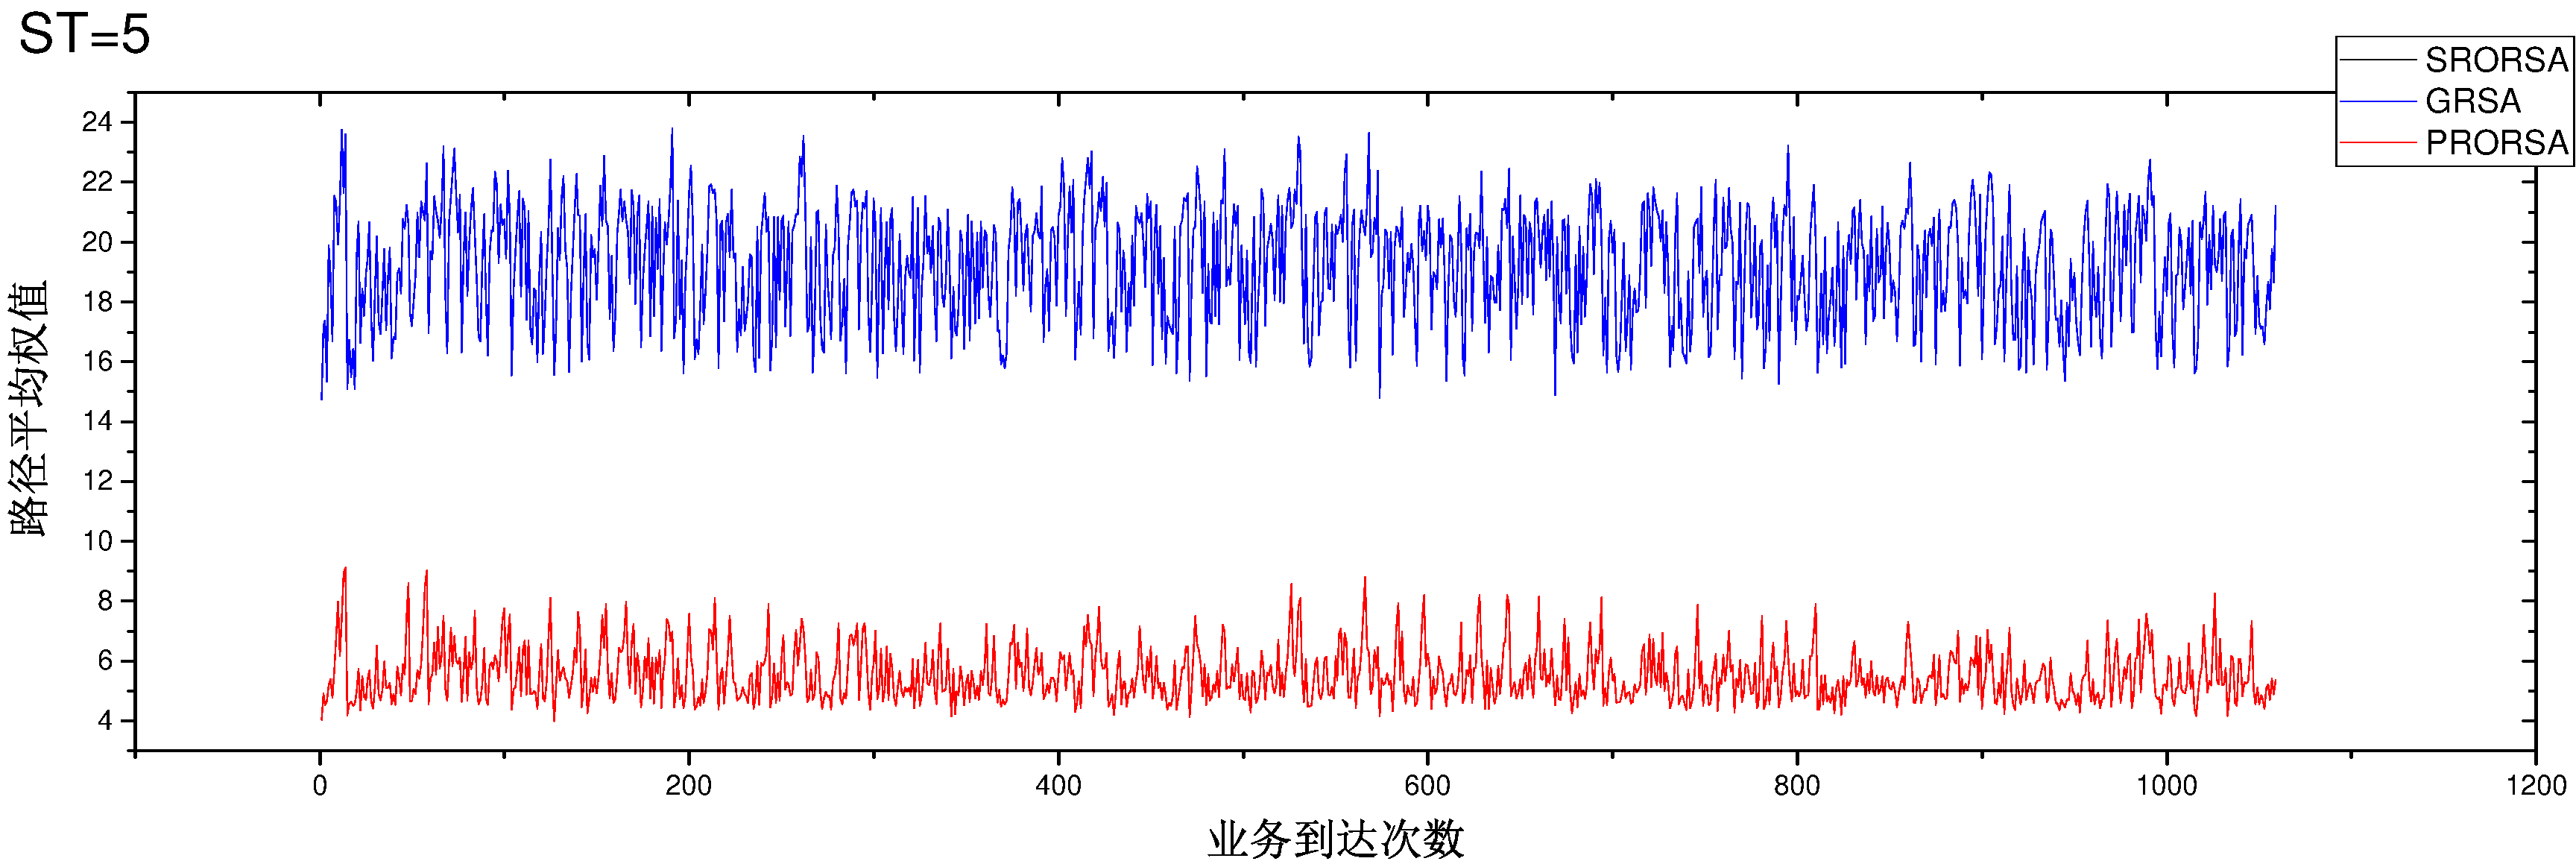
\includegraphics[width=1 \textwidth]{figures/H5C.pdf}}
\end{center}
\caption{{\footnotesize{带权图路径权值对比(ST=5)}}}
\label{H5C}
\end{figure*}
\begin{figure*}
\setlength{\belowcaptionskip}{-0.5cm}
\begin{center}
{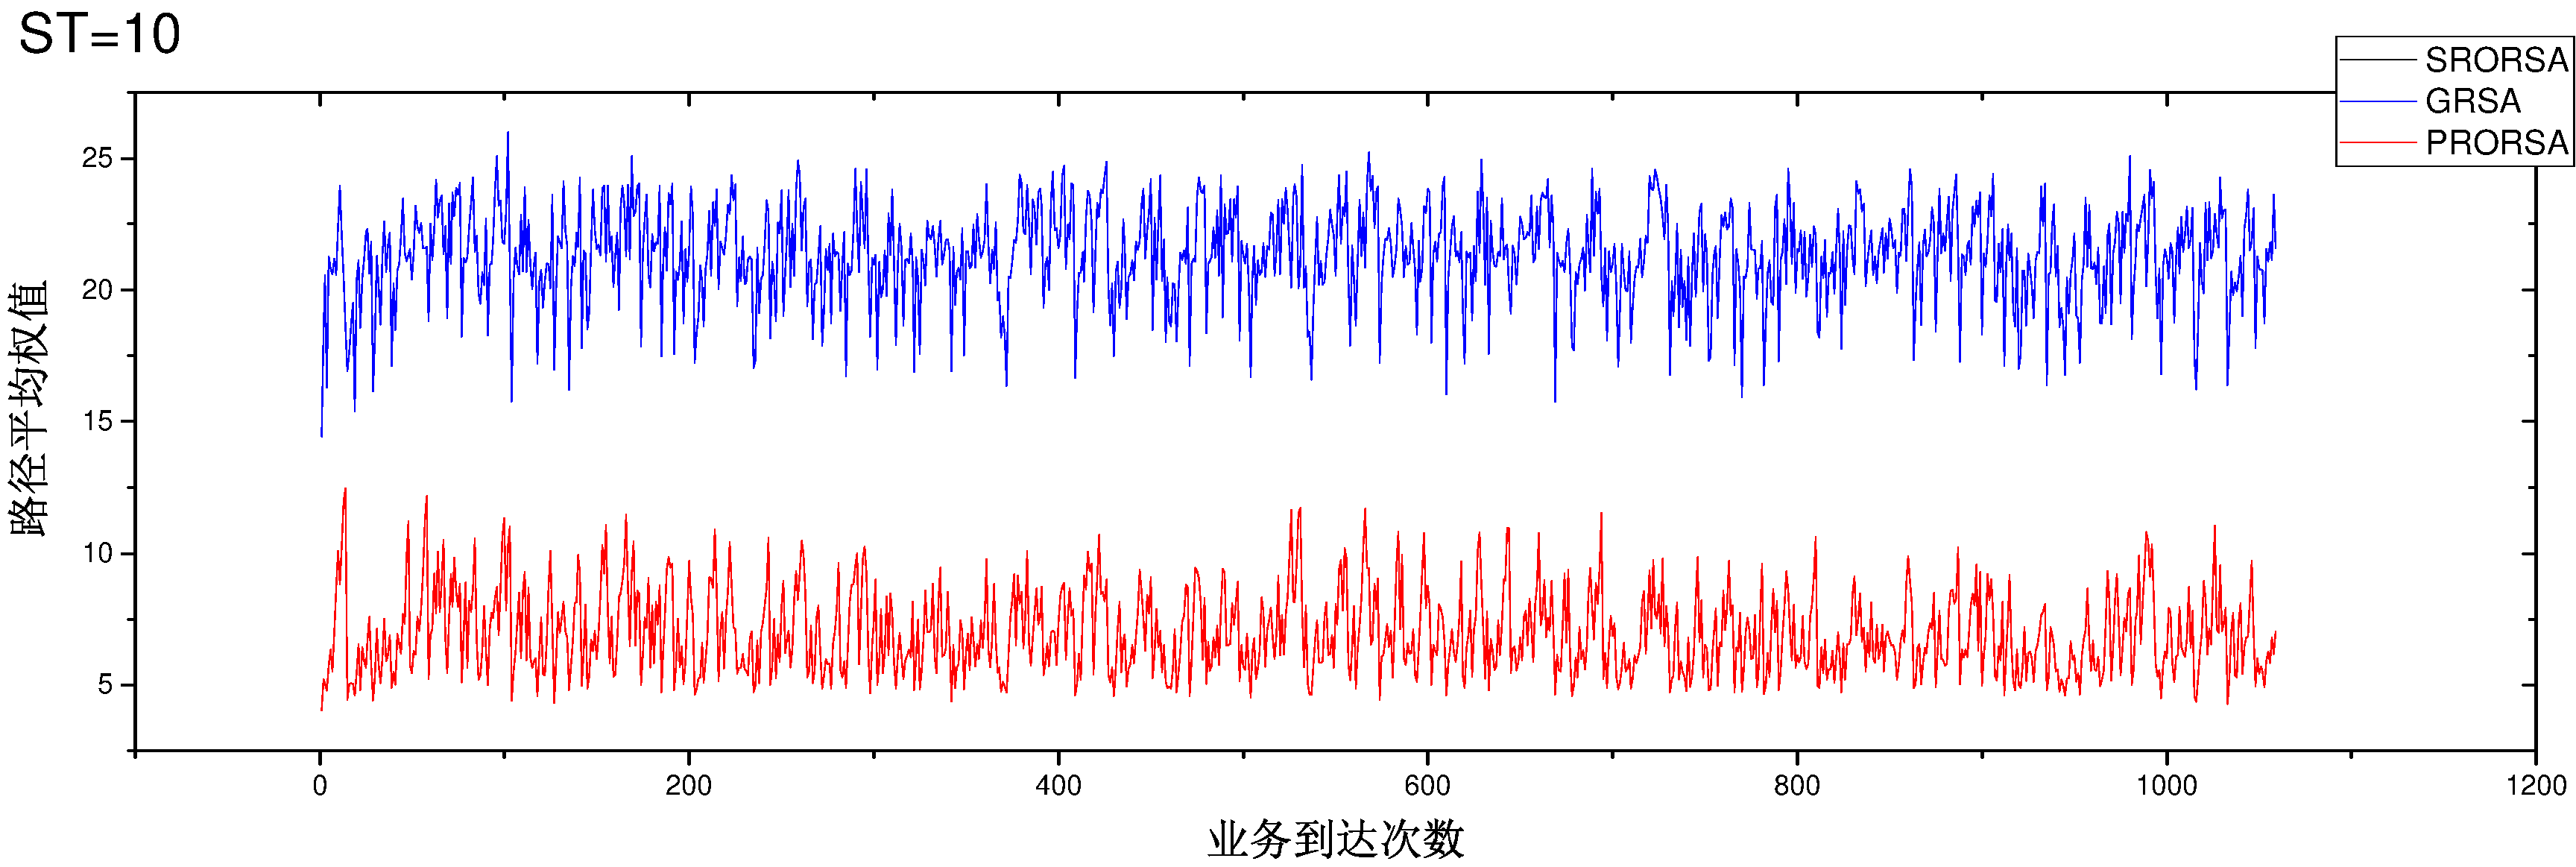
\includegraphics[width=1 \textwidth]{figures/H10C.pdf}}
\end{center}
\caption{{\footnotesize{带权图路径权值对比(ST=10)}}}
\label{H10C}
\end{figure*}
\begin{figure*}
\setlength{\belowcaptionskip}{-0.5cm}
\begin{center}
{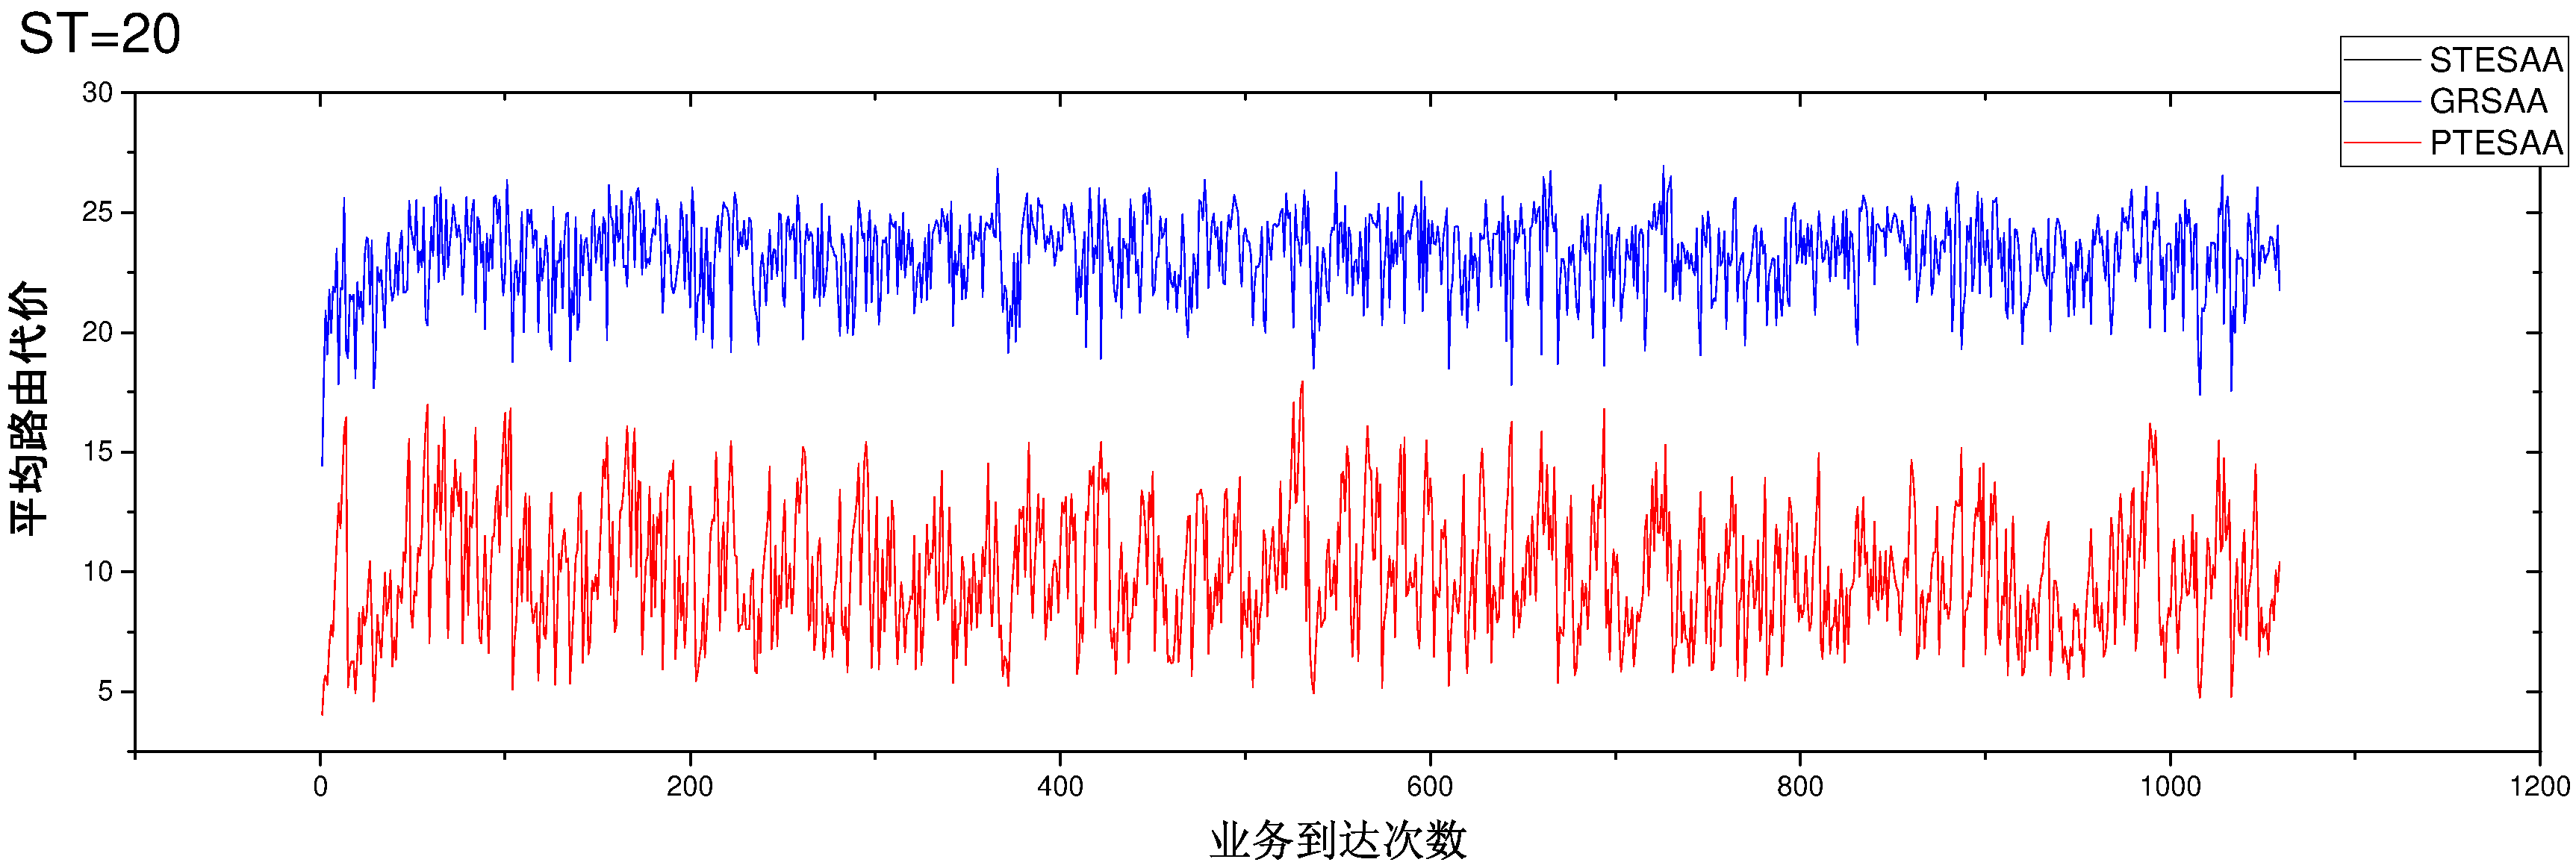
\includegraphics[width=1 \textwidth]{figures/H20C.pdf}}
\end{center}
\caption{{\footnotesize{带权图路径权值对比(ST=20)}}}
\label{H20C}
\end{figure*}
\begin{figure*}
\setlength{\belowcaptionskip}{-0.5cm}
\begin{center}
{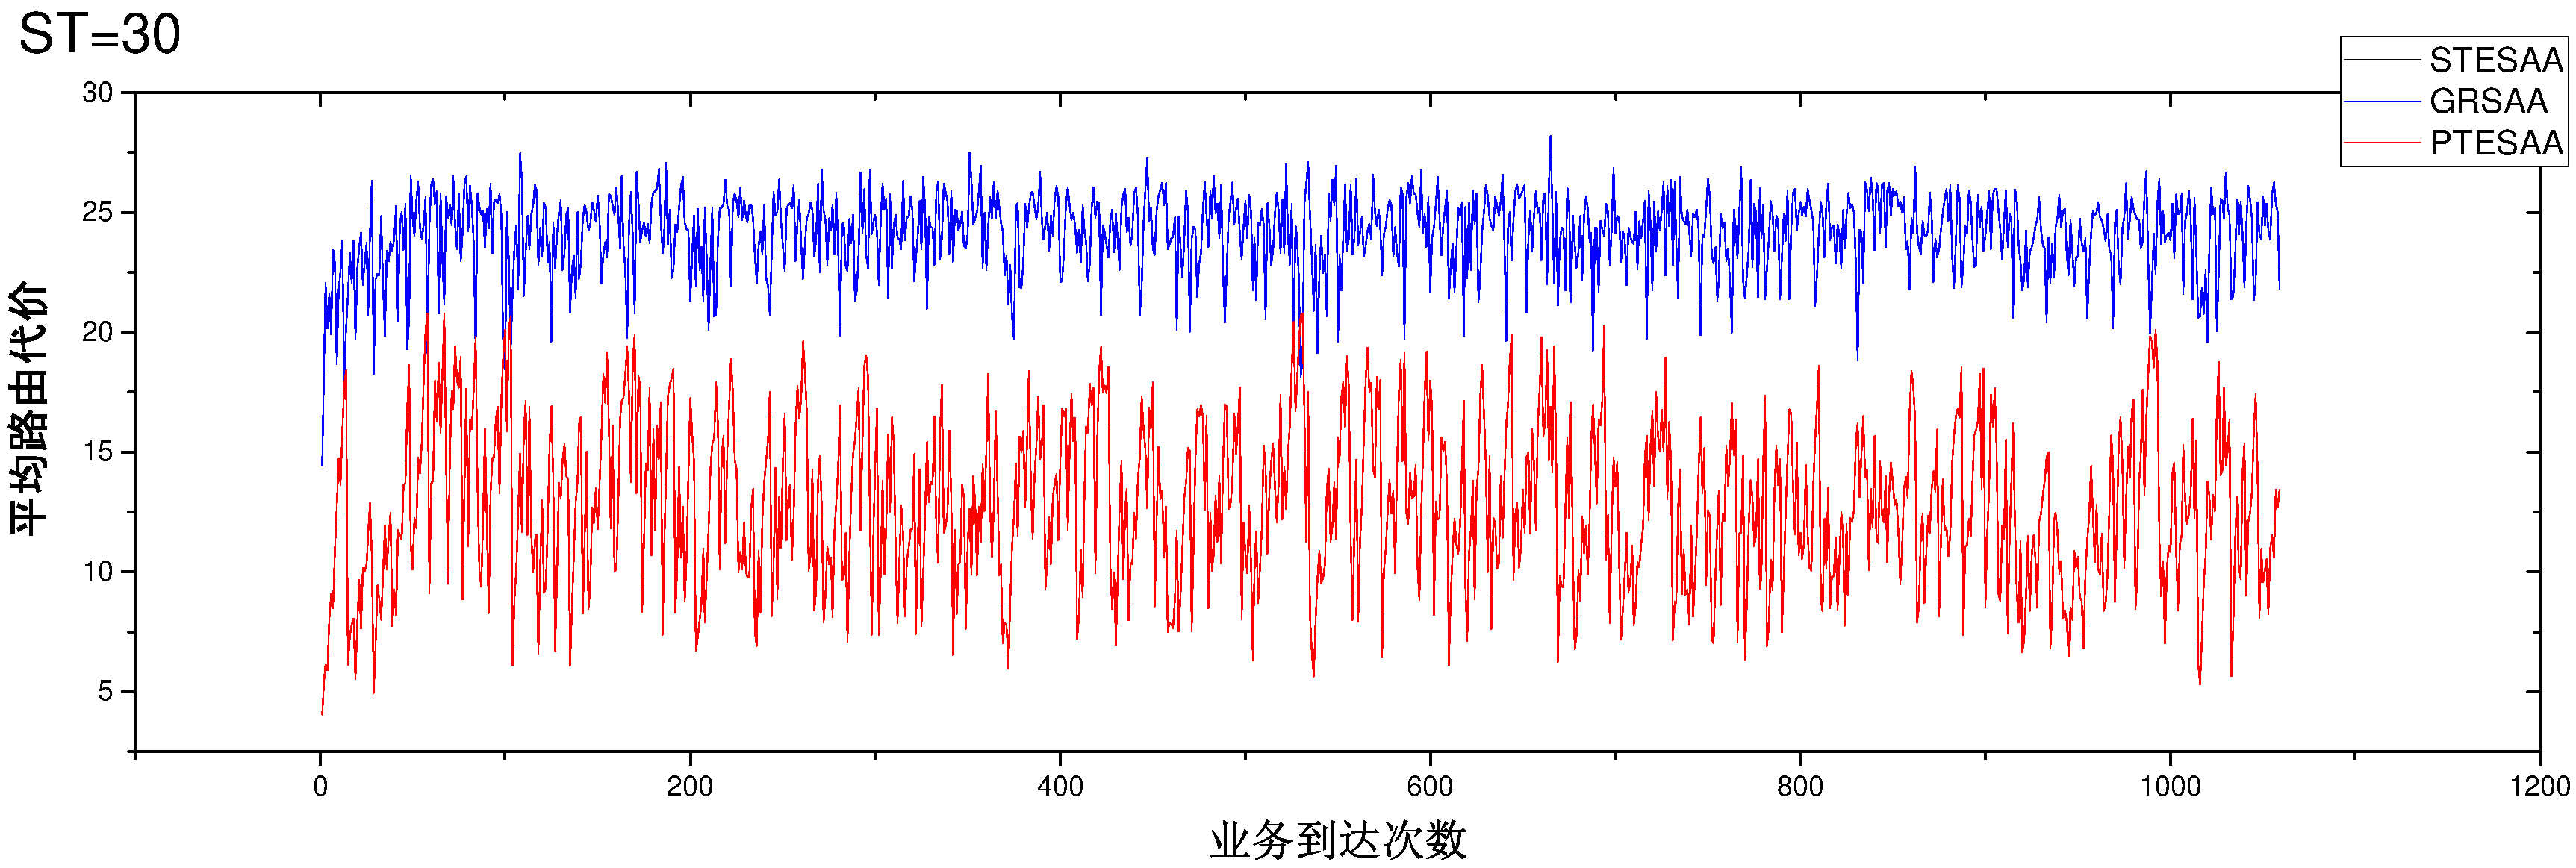
\includegraphics[width=1 \textwidth]{figures/H30C.pdf}}
\end{center}
\caption{{\footnotesize{带权图路径权值对比(ST=30)}}}
\label{H30C}
\end{figure*}
\begin{figure*}
\setlength{\belowcaptionskip}{-0.5cm}
\begin{center}
{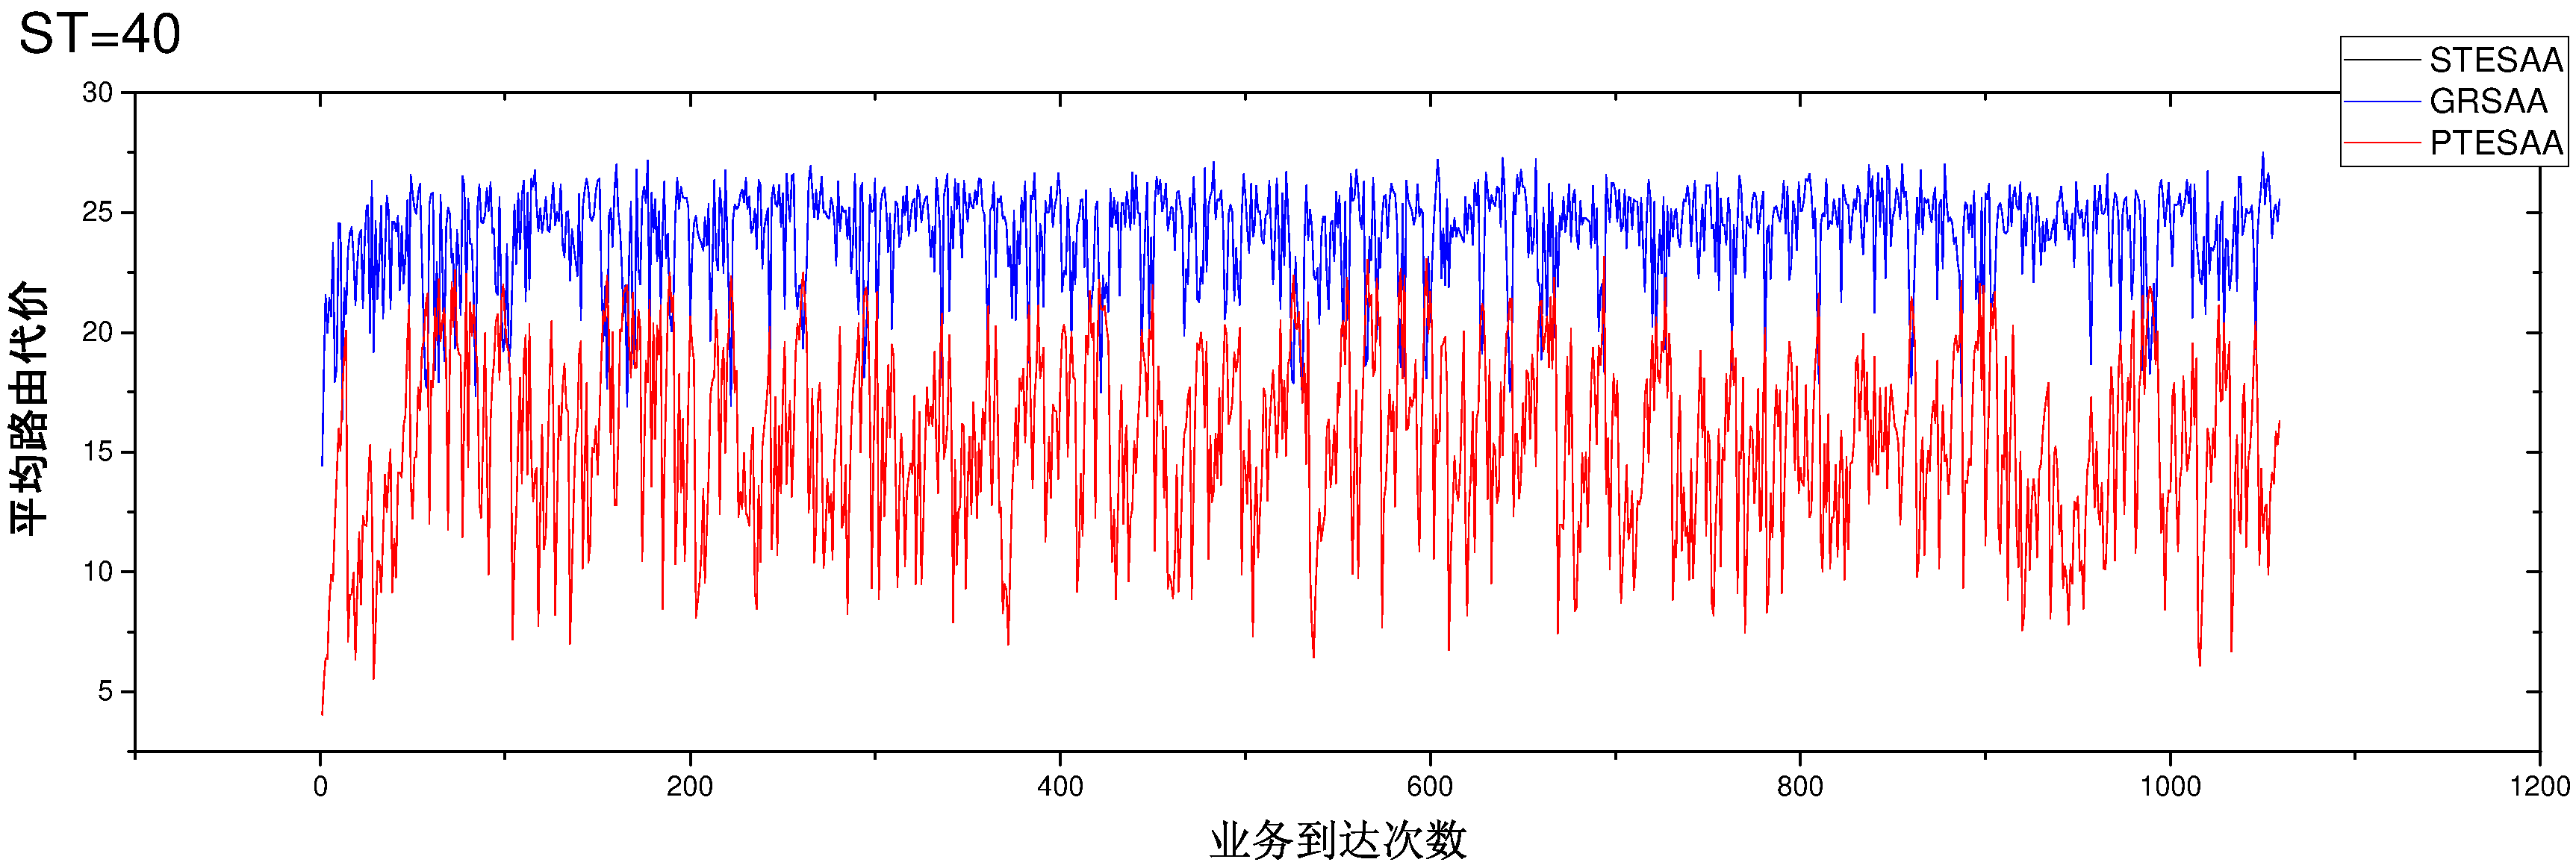
\includegraphics[width=1 \textwidth]{figures/H40C.pdf}}
\end{center}
\caption{{\footnotesize{带权图路径权值对比(ST=40)}}}
\label{H40C}
\end{figure*}

图 \ref{H5C}到图 \ref{H40C}表示了权值的优化结果,我们把PRORSA和SRORSA的优化结果与贪心算法GRSA的算法权值优化结果进行比较,图中的横坐标表示业务到达的次数,一共产生1051个加入事件,网络链路的权值设置为1到10之间的整数值,当网络状况较好的时候,比如,平均服务时间为$ST=5$ 时,路径权值达到了平均3.5倍的优化,PRORSA和SRORSA 的权值在3-10 之间波动,把业务的路径权值控制在很小的范围,路径优化得非常的理想。另外,随着平均服务时间$ST$ 的增加,贪心算法GRSA的路径平均权值轻微增加,由平均20增加到平均25,这是因为GRSA 是贪心的利用分层图,对链路的权值大小没有限制,不管在拥塞和不拥塞的网络条件下都会产生大量高权值的路径。观察PRORSA 和SRORSA 路径权值随着$ST$ 的变化发现,PRORSA 和SRORSA 的链路权值随着$ST$的增加而不断上涨,从最初的均值为7 到最后($ST=40$) 时的均值为15,这是因为当网络压力较大时,网络中的可用链路会出现匮乏,每个分层图上的路径权值都会很大,使得优化选择的空间变小。
\begin{figure*}
\setlength{\belowcaptionskip}{-0.5cm}
\begin{center}
{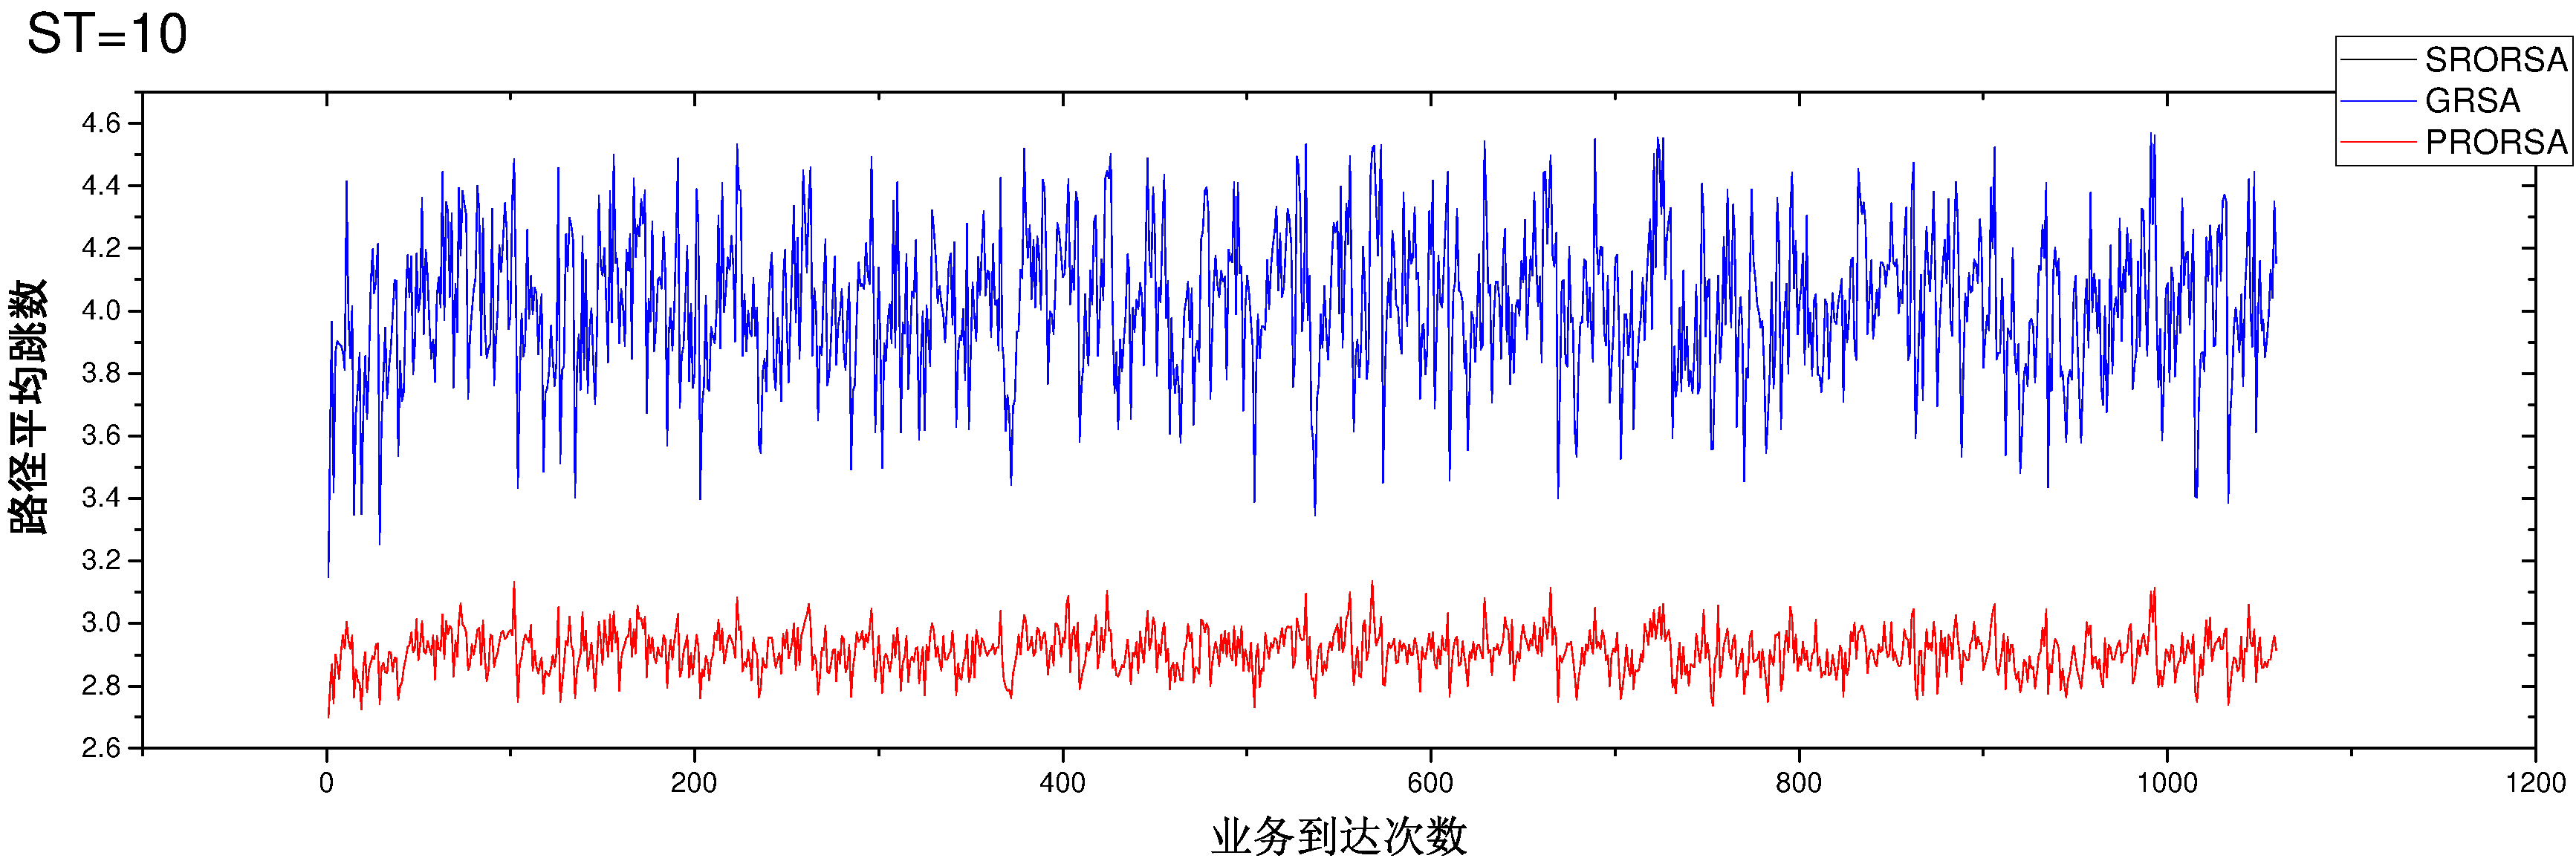
\includegraphics[width=1 \textwidth]{figures/H10H.pdf}}
\end{center}
\caption{{\footnotesize{带权图路径跳数对比(ST=10)}}}
\label{H10H}
\end{figure*}
\begin{figure*}
\setlength{\belowcaptionskip}{-0.5cm}
\begin{center}
{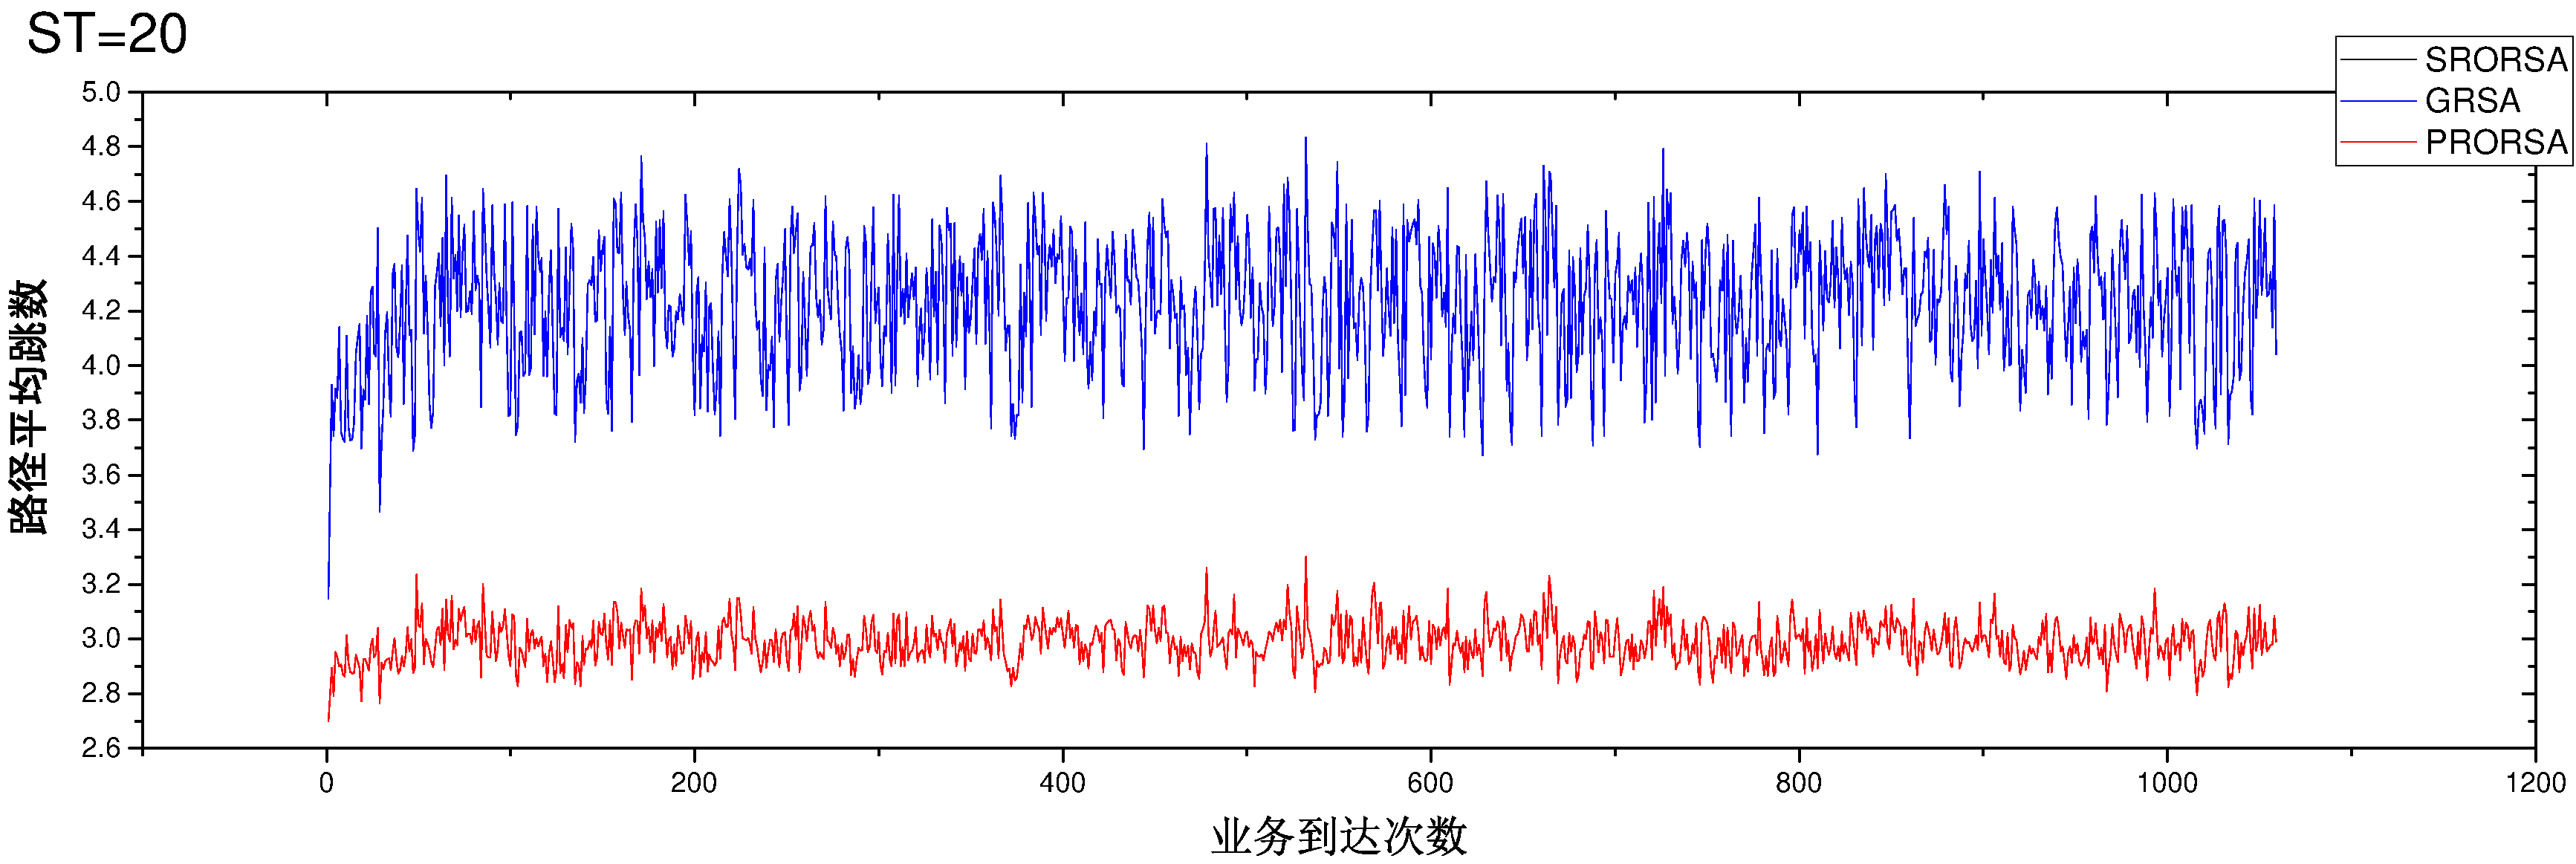
\includegraphics[width=1 \textwidth]{figures/H20H.pdf}}
\end{center}
\caption{{\footnotesize{带权图路径跳数对比(ST=20)}}}
\label{H20H}
\end{figure*}
\begin{figure*}
\setlength{\belowcaptionskip}{-0.5cm}
\begin{center}
{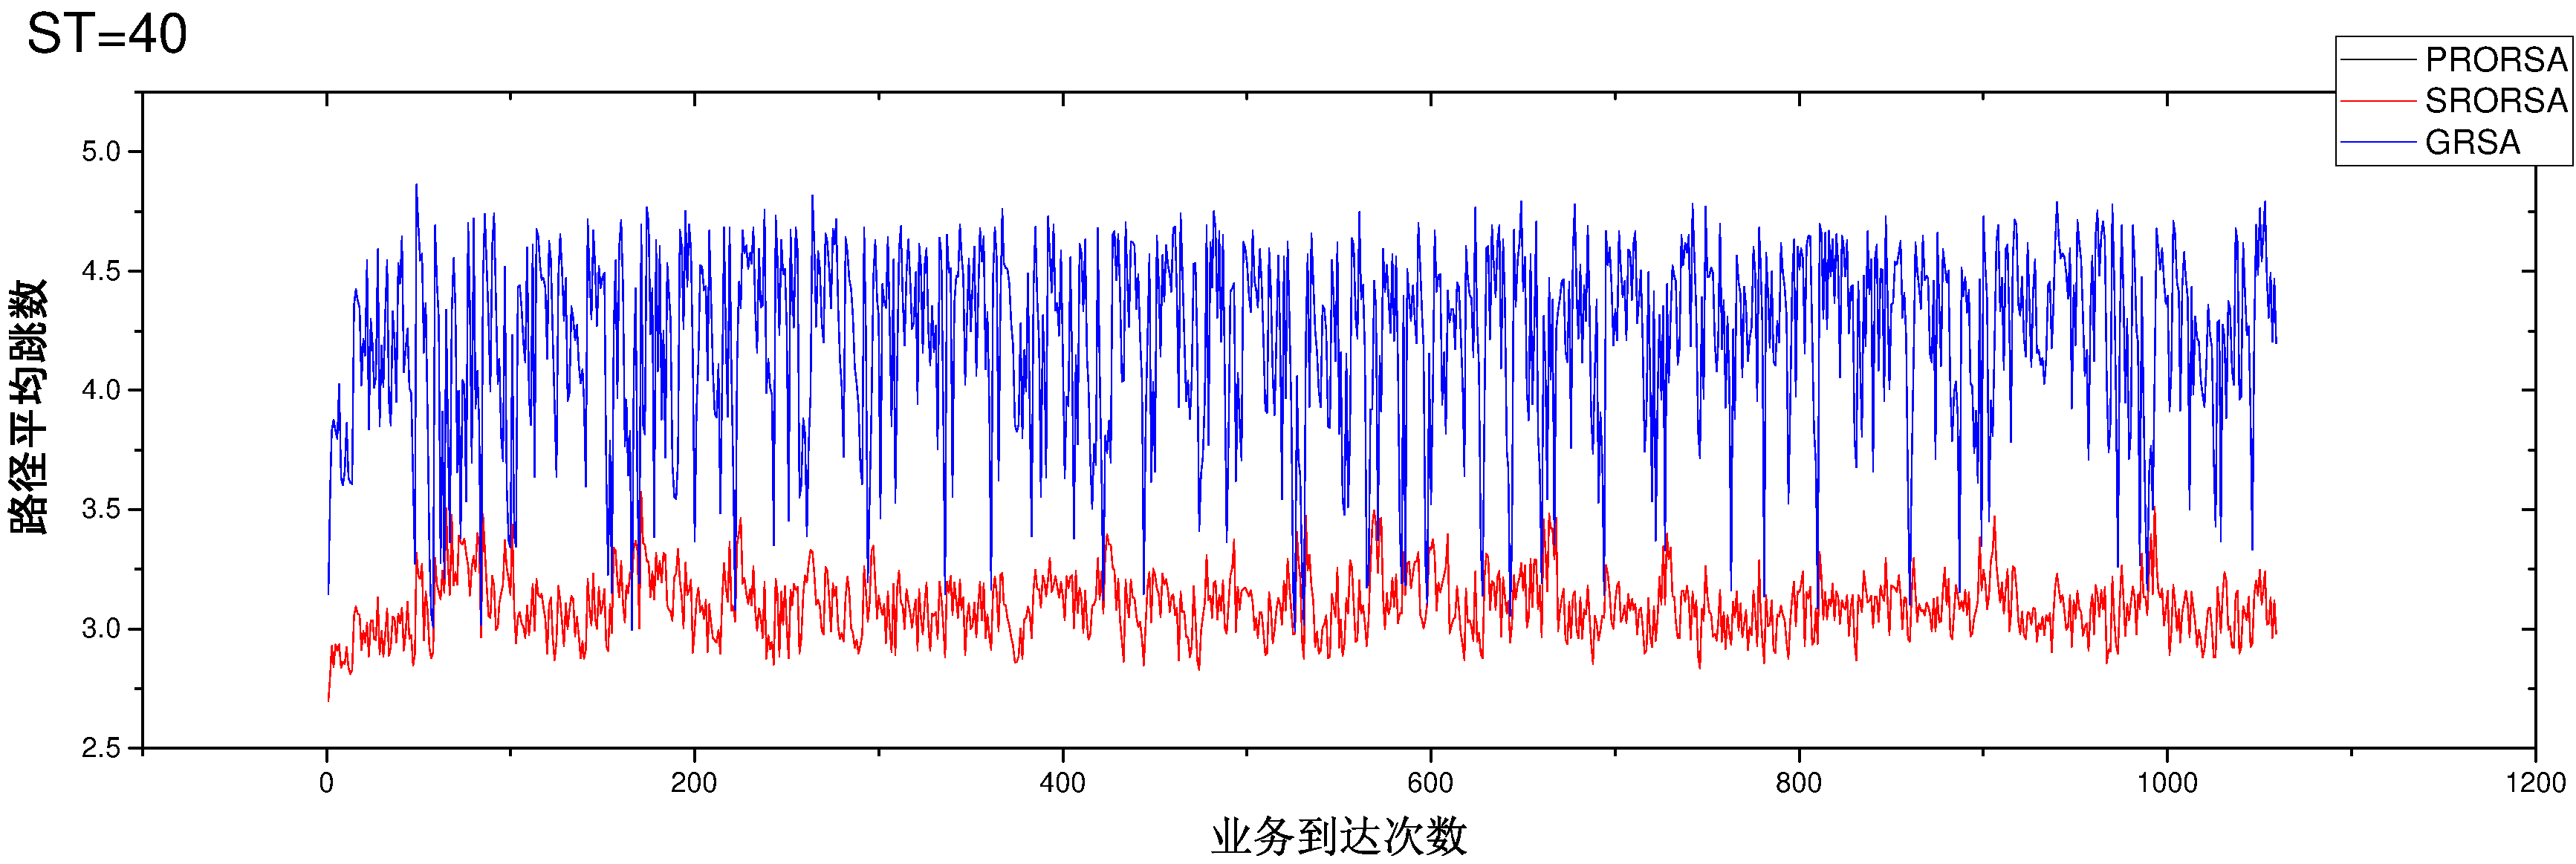
\includegraphics[width=1 \textwidth]{figures/H40H.pdf}}
\end{center}
\caption{{\footnotesize{带权图路径跳数对比(ST=40)}}}
\label{H40H}
\end{figure*}

图 \ref{H10H}到 \ref{H40H}显示了带权情况下的路径跳数情况,可以看到当权值优化时,业务的跳数也得到了很大的优化,这是因为权值小的路径常常路跳径较短,而且GRSA是会贪心的在一个分层图上加入业务,导致分层图变得碎片化,容易求得跳数较大的路径,所以即使在带权图的优化中,跳数也会减小很大。
\subsubsection{时间分析}

图 \ref{H5T}到图 \ref{H40T}展示了在不同平均服务时间$ST$下的各种算法的计算时间,当$ST=5$时,我们可以看到通过GPU加速的PRORSA的计算时间是SPROA 的计算时间的1/4,而实际上备选路径部分的GPU加速达到了7-8 倍,但是由于步骤二的快速路径选择过程也需要消耗一部分时间,这部分时间不能进行GPU加速,实际上PRORSA的大部分算法时间花在了步骤二的路径选择上,所以使得总体的加速比下降为4 倍左右。我们发现由于PRORSA的波动幅度比SRORSA的波动幅度小很多,这是因为SRORSA的大部分时间花在计算备选路上,备选路径的计算量随着业务数量和网络链路的占用情况变化较大,而PRORSA的计算量花在步骤二上,计算量变化较小。GRSA的计算时间略高于PRORSA的计算时间,而且GRSA的波动幅度很大,不够平稳,这是因为GRSA贪心策略占用链路资源过多,容易造成分层图链路的碎片化,使得计算量变化较大。
观察到随着$ST$的变化PRORSA的对SRORSA的加速比逐渐下降,这是因为随着网络压力的增加,可用链路变少,使得SRORSA的备选路径计算复杂度下降,PRORSA加速优势变小。另外,随着$ST$的增加,PRORSA 和SRORSA的波动幅度增加,这是因为由于链路繁忙,使得大量业务不能一次性加入,步骤二到步骤一之间的循环次数增加,使得某些业务到达点的业务需要多次的循环,计算时间变长。
\begin{figure*}
\setlength{\belowcaptionskip}{-0.5cm}
\begin{center}
{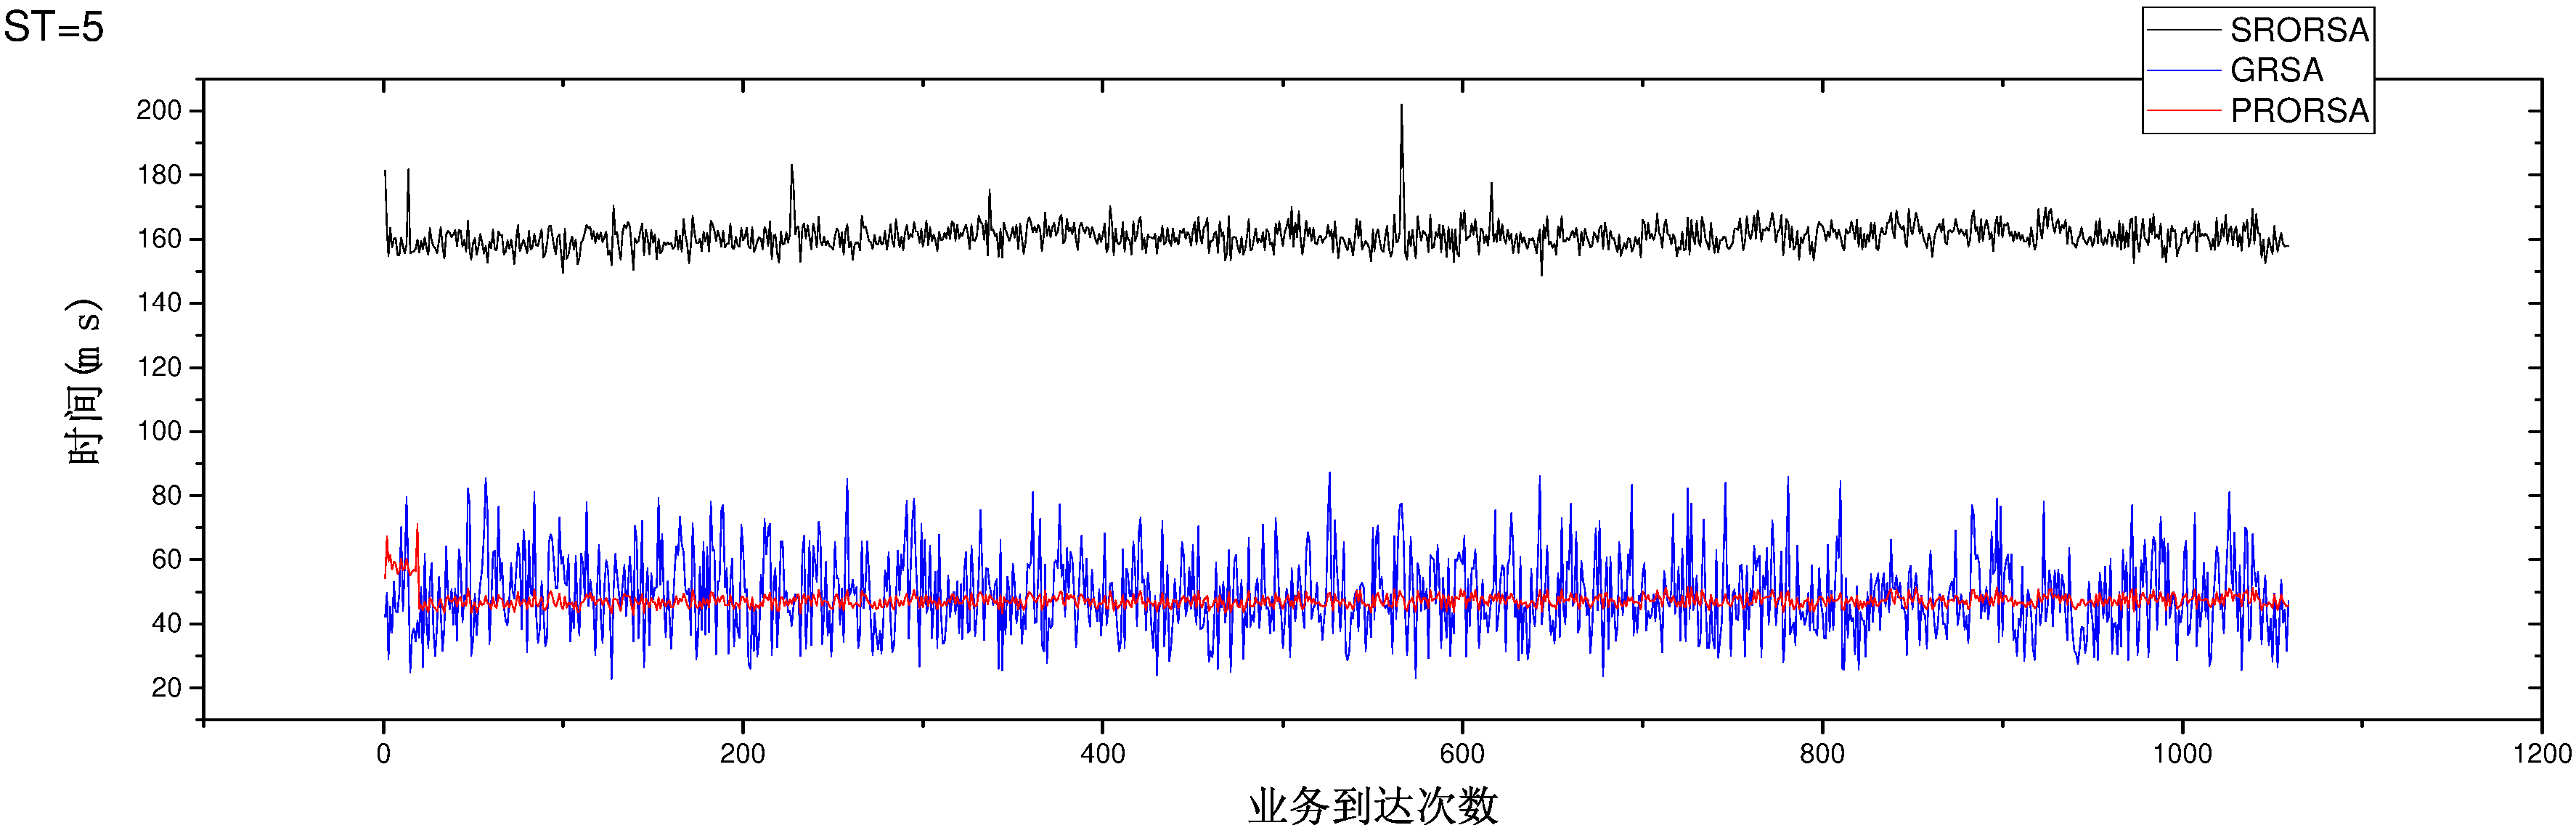
\includegraphics[width=1 \textwidth]{figures/H5T.pdf}}
\end{center}
\caption{{\footnotesize{带权图时间对比(ST=5)}}}
\label{H5T}
\end{figure*}
\begin{figure*}
\setlength{\belowcaptionskip}{-0.5cm}
\begin{center}
{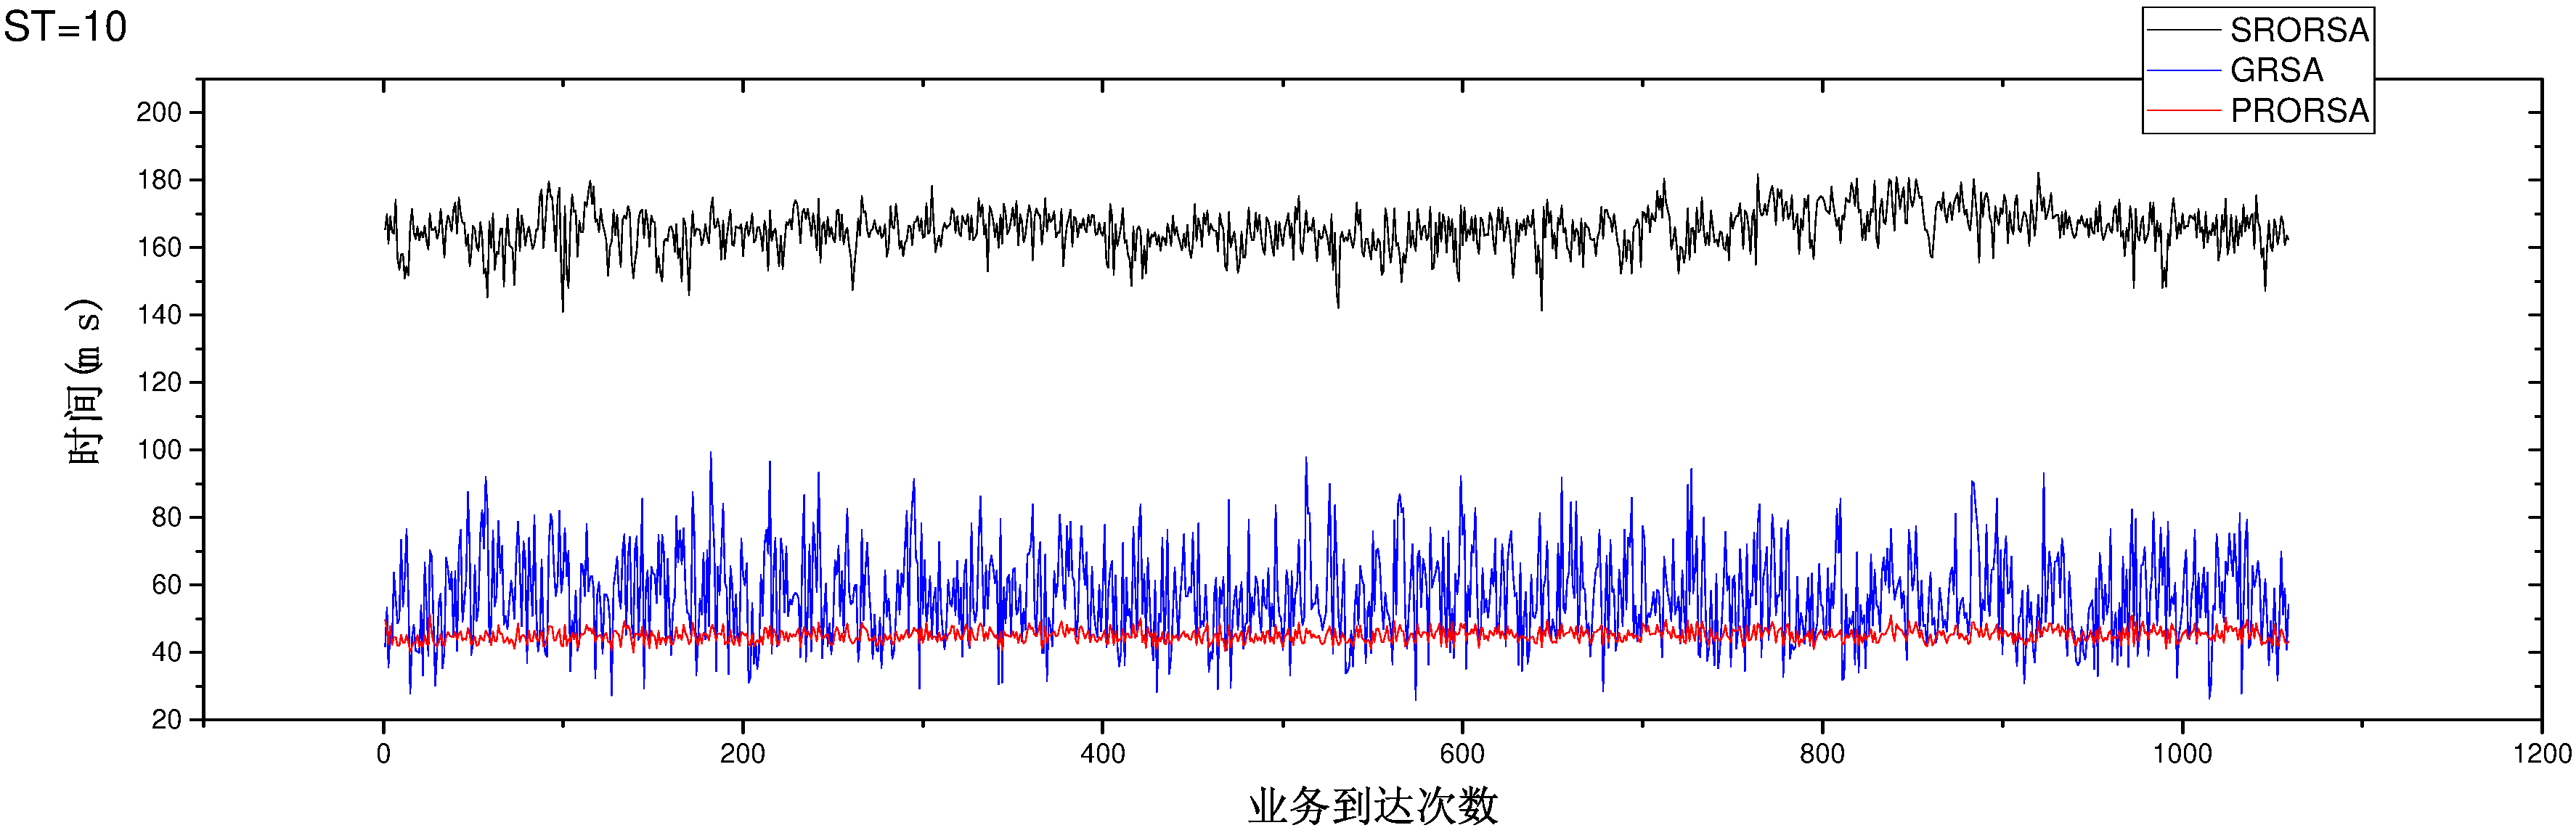
\includegraphics[width=1 \textwidth]{figures/H10T.pdf}}
\end{center}
\caption{{\footnotesize{带权图时间对比(ST=10)}}}
\label{H10T}
\end{figure*}
\begin{figure*}
\setlength{\belowcaptionskip}{-0.5cm}
\begin{center}
{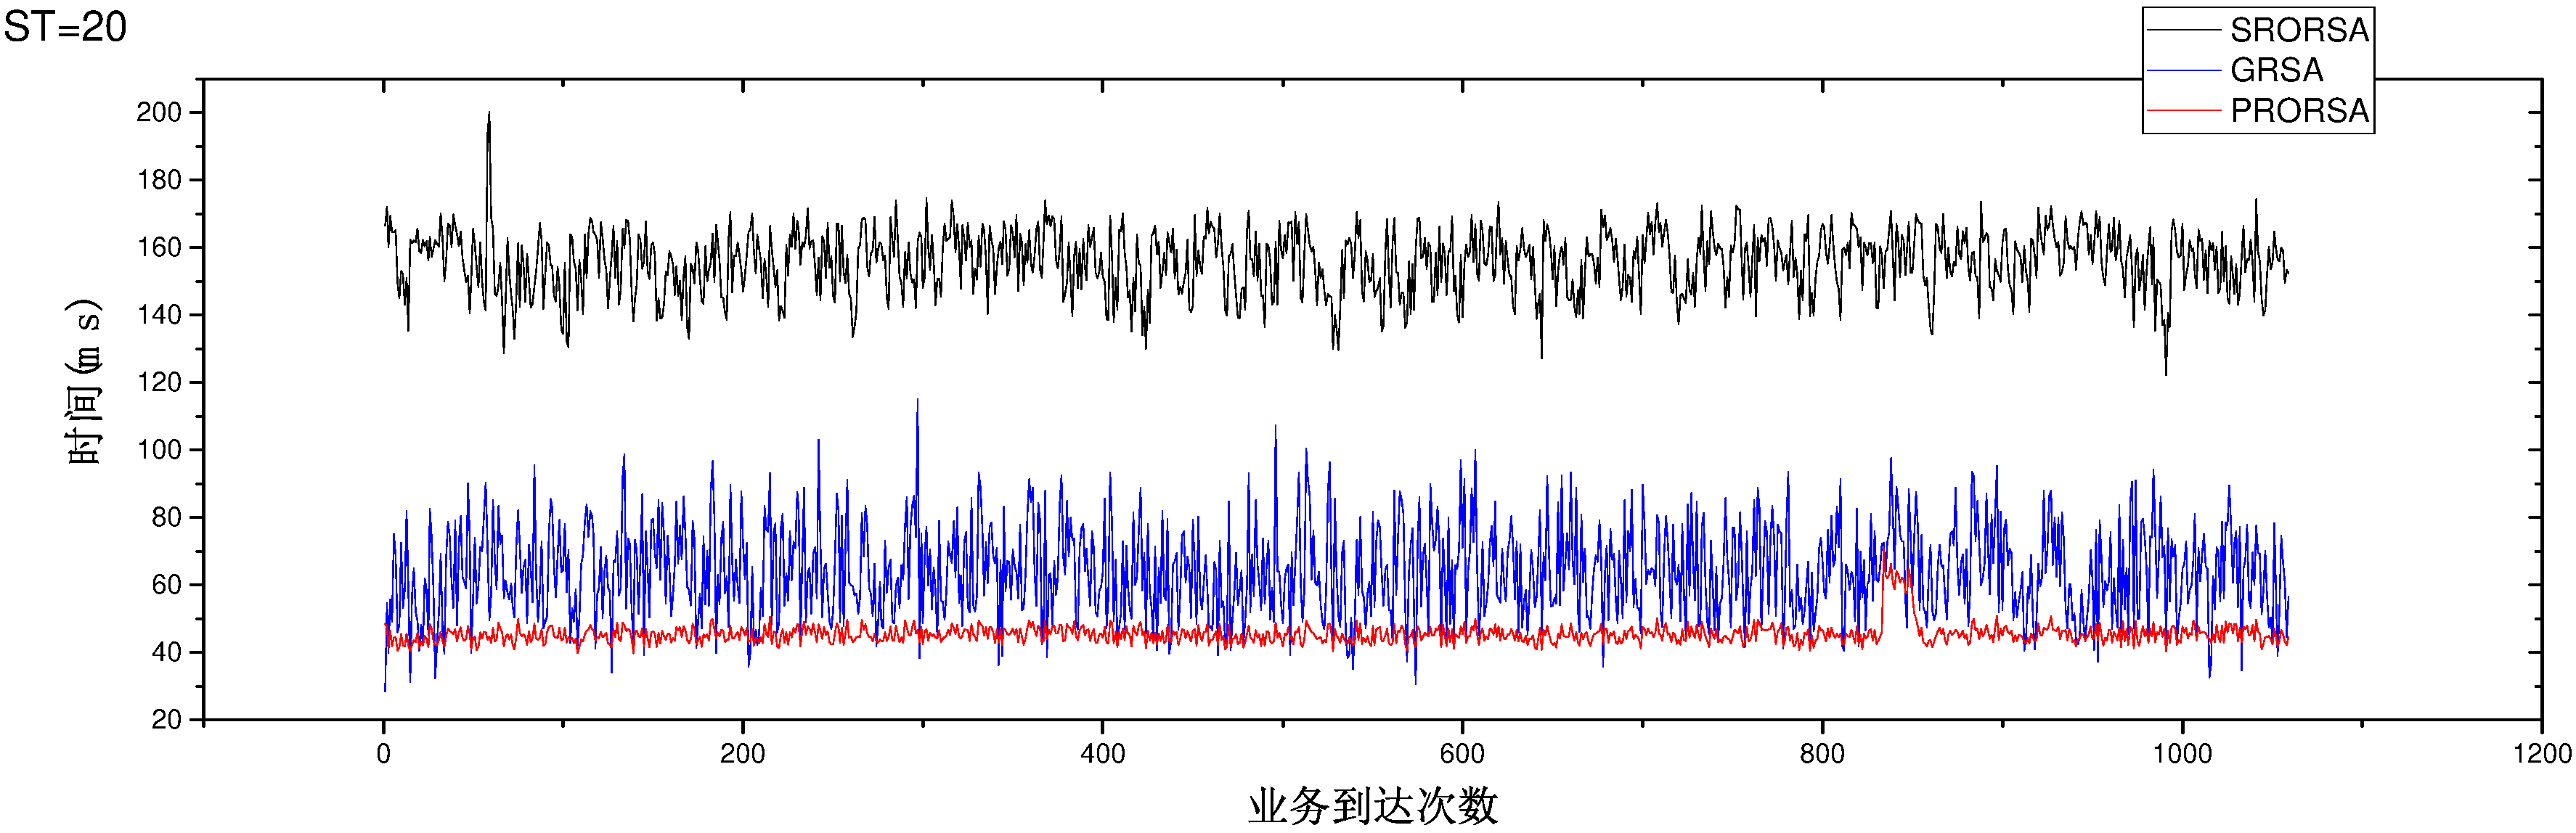
\includegraphics[width=1 \textwidth]{figures/H20T.pdf}}
\end{center}
\caption{{\footnotesize{带权图时间对比(ST=20)}}}
\label{H20T}
\end{figure*}
\begin{figure*}
\setlength{\belowcaptionskip}{-0.5cm}
\begin{center}
{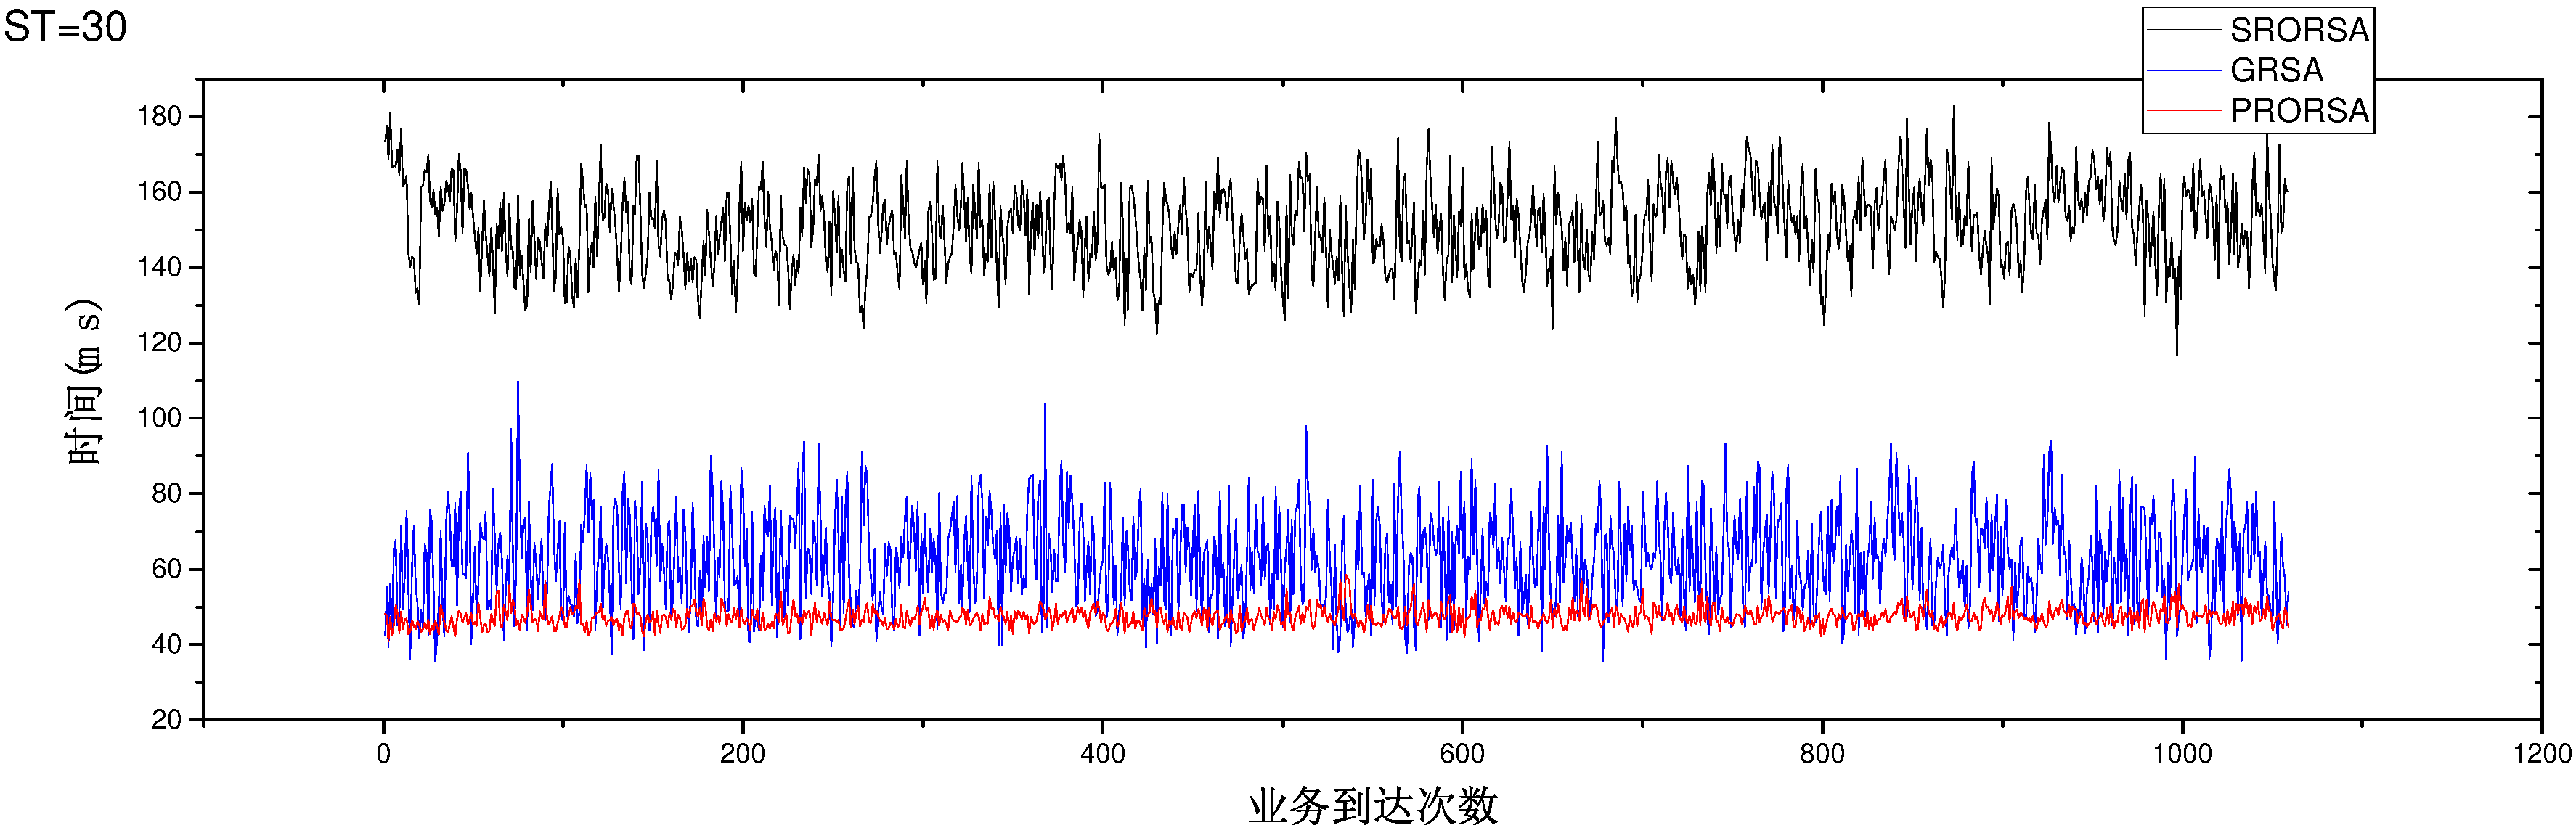
\includegraphics[width=1 \textwidth]{figures/H30T.pdf}}
\end{center}
\caption{{\footnotesize{带权图时间对比(ST=30)}}}
\label{H30T}
\end{figure*}
\begin{figure*}
\setlength{\belowcaptionskip}{-0.5cm}
\begin{center}
{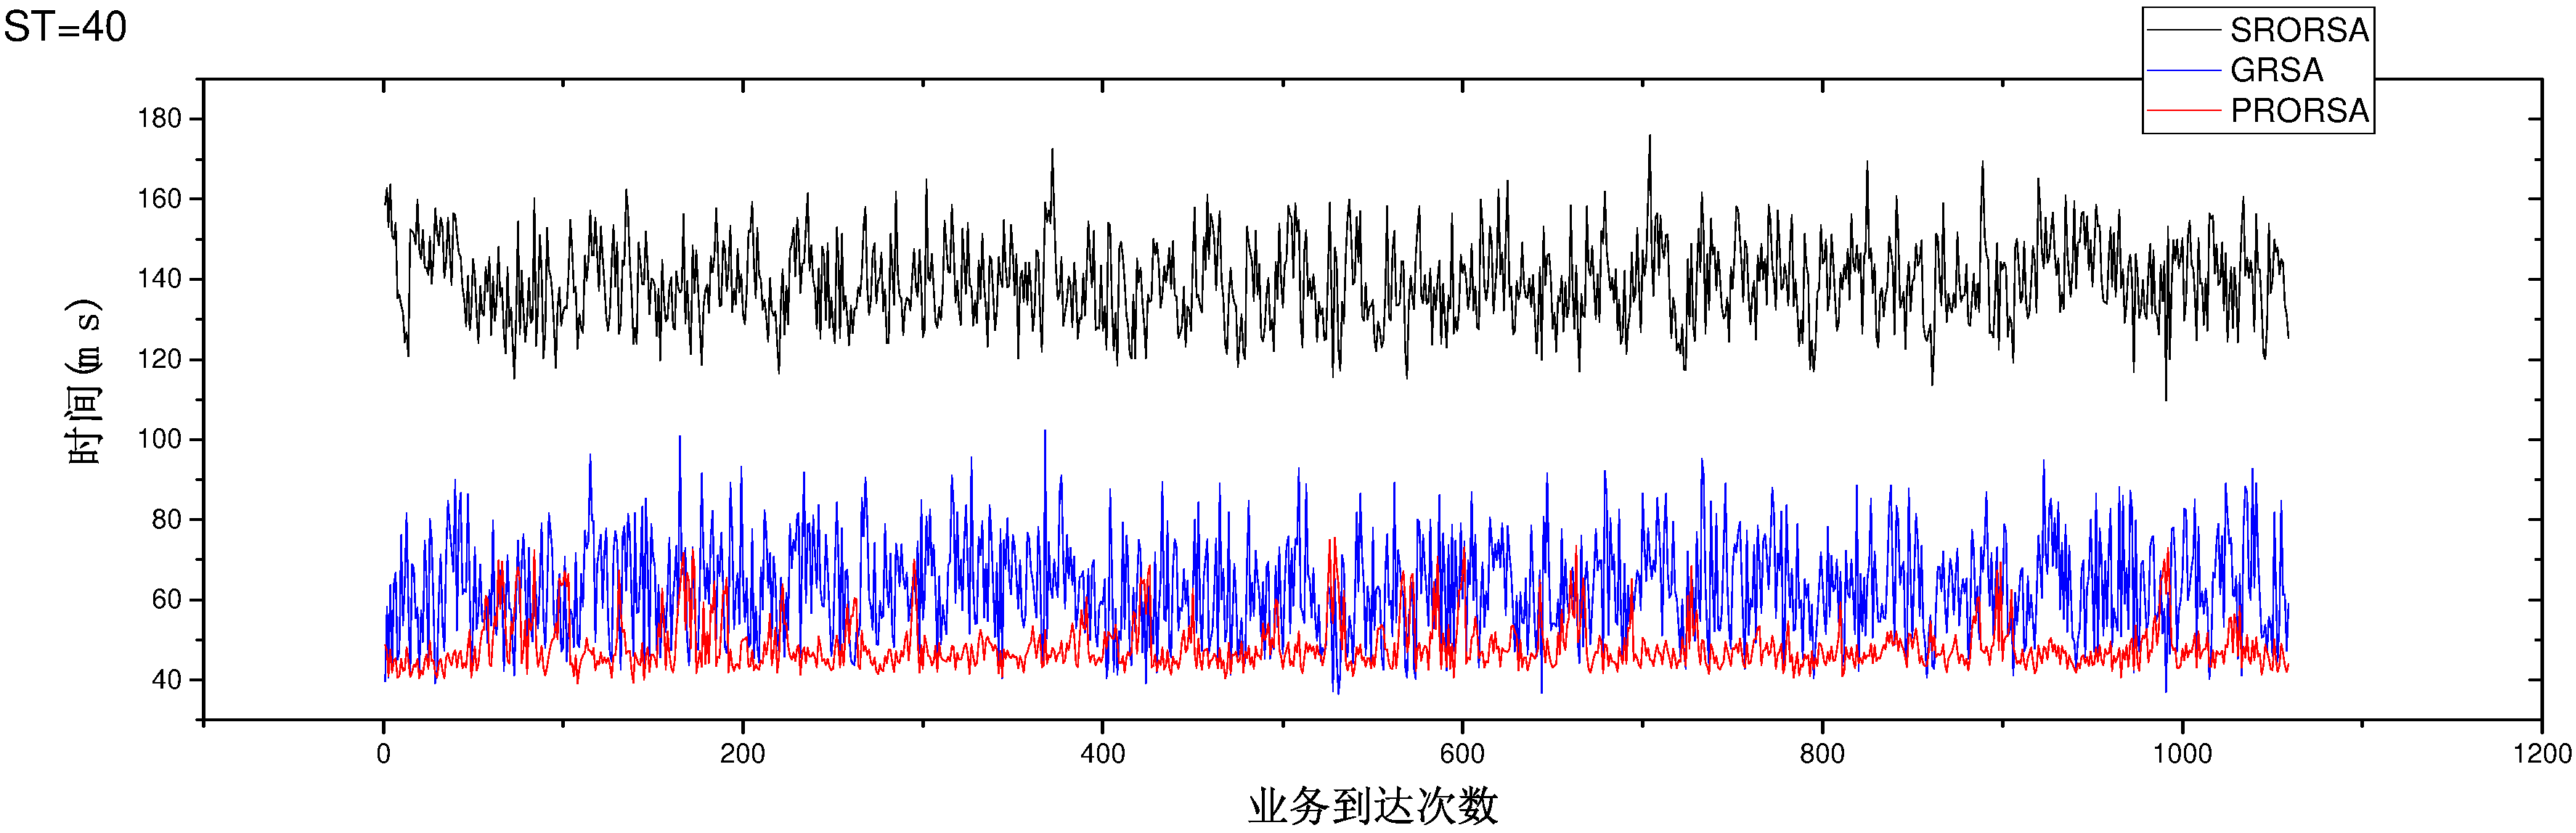
\includegraphics[width=1 \textwidth]{figures/H40T.pdf}}
\end{center}
\caption{{\footnotesize{带权图时间对比(ST=40)}}}
\label{H40T}
\end{figure*}
\subsubsection{阻塞率分析}

图 \ref{H10Z}到图 \ref{H40Z}展示了带权情况下随着$ST$的变化,PRORSA,SRORSA和GRSA的阻塞率变化情况,由于带权情况下的跳数也优化得很理想,所以其占用的链路资源也较少,阻塞情况得到改善。当$ST=10$时,我们发现PRORSA/SRORSA 的阻塞次数明显小于GRSA。 当$ST=20$ 时,PRORSA/SRORSA 的阻塞次数和阻塞幅度均小于GRSA,在GRSA中出现了一次相对较大的阻塞,但是PRORSA/SRORSA 中没有出现这种不平稳的阻塞率突变。当$ST=30$ 时,我们发现PRORSA/SRORSA的阻塞次数和阻塞幅度比GRSA小很多,GRSA的平均阻塞率是PRORSA/SRORSA的6倍左右。当$ST=40$时,PRORSA,SRORSA和GRSA 的阻塞率都增加很多,但是PRORSA/SRORSA的阻塞情况还是大大优于GRSA。
\begin{figure*}
\setlength{\belowcaptionskip}{-0.5cm}
\begin{center}
{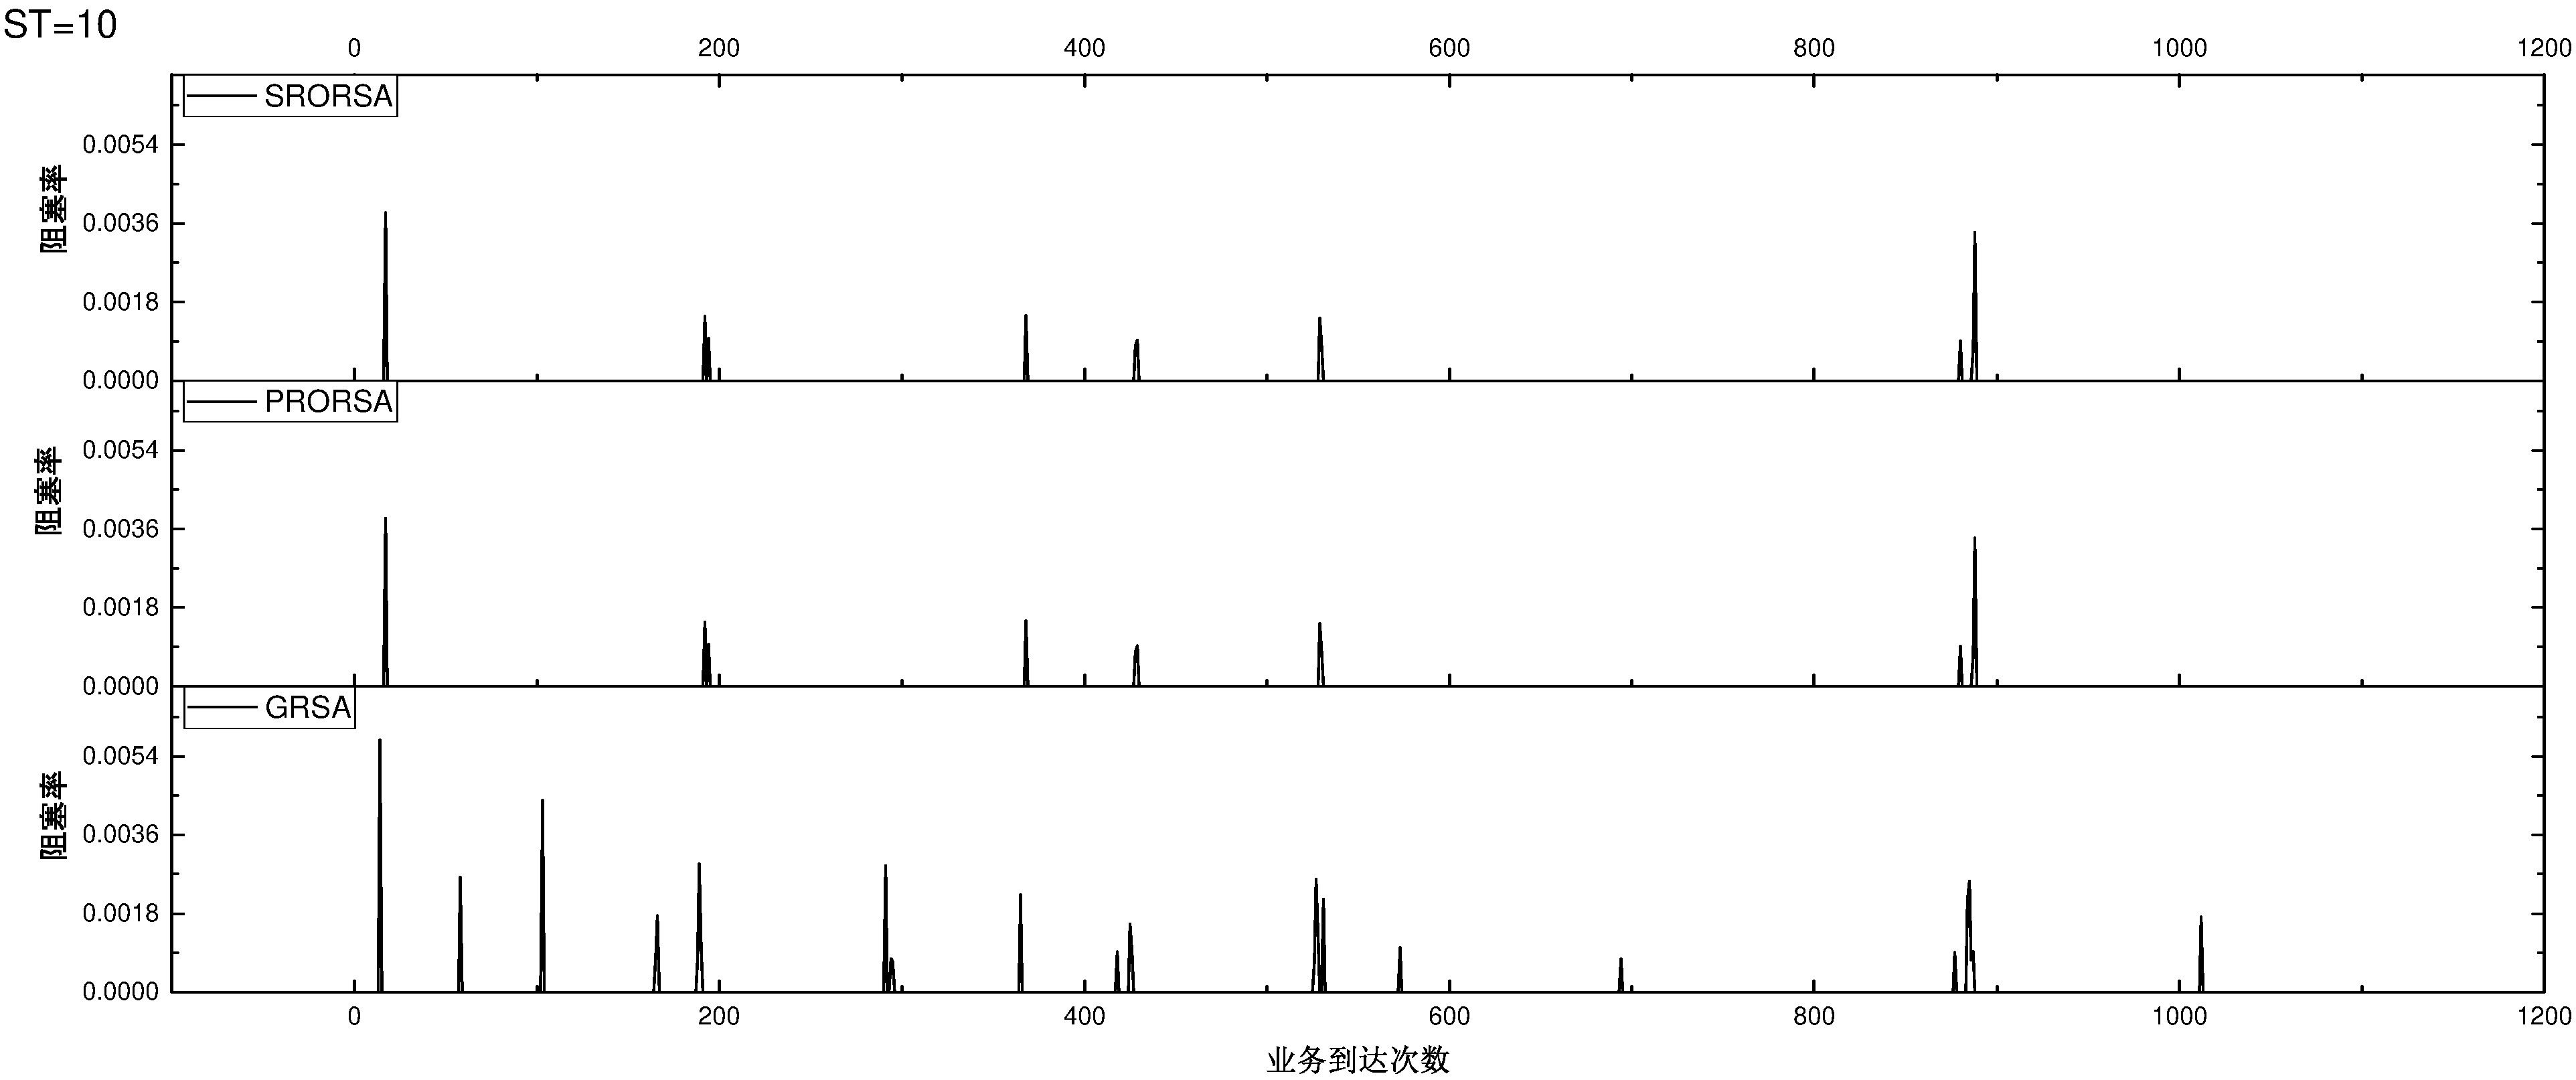
\includegraphics[width=1 \textwidth]{figures/H10Z.pdf}}
\end{center}
\caption{{\footnotesize{带权图阻塞率对比(ST=10)}}}
\label{H10Z}
\end{figure*}
\begin{figure*}
\setlength{\belowcaptionskip}{-0.5cm}
\begin{center}
{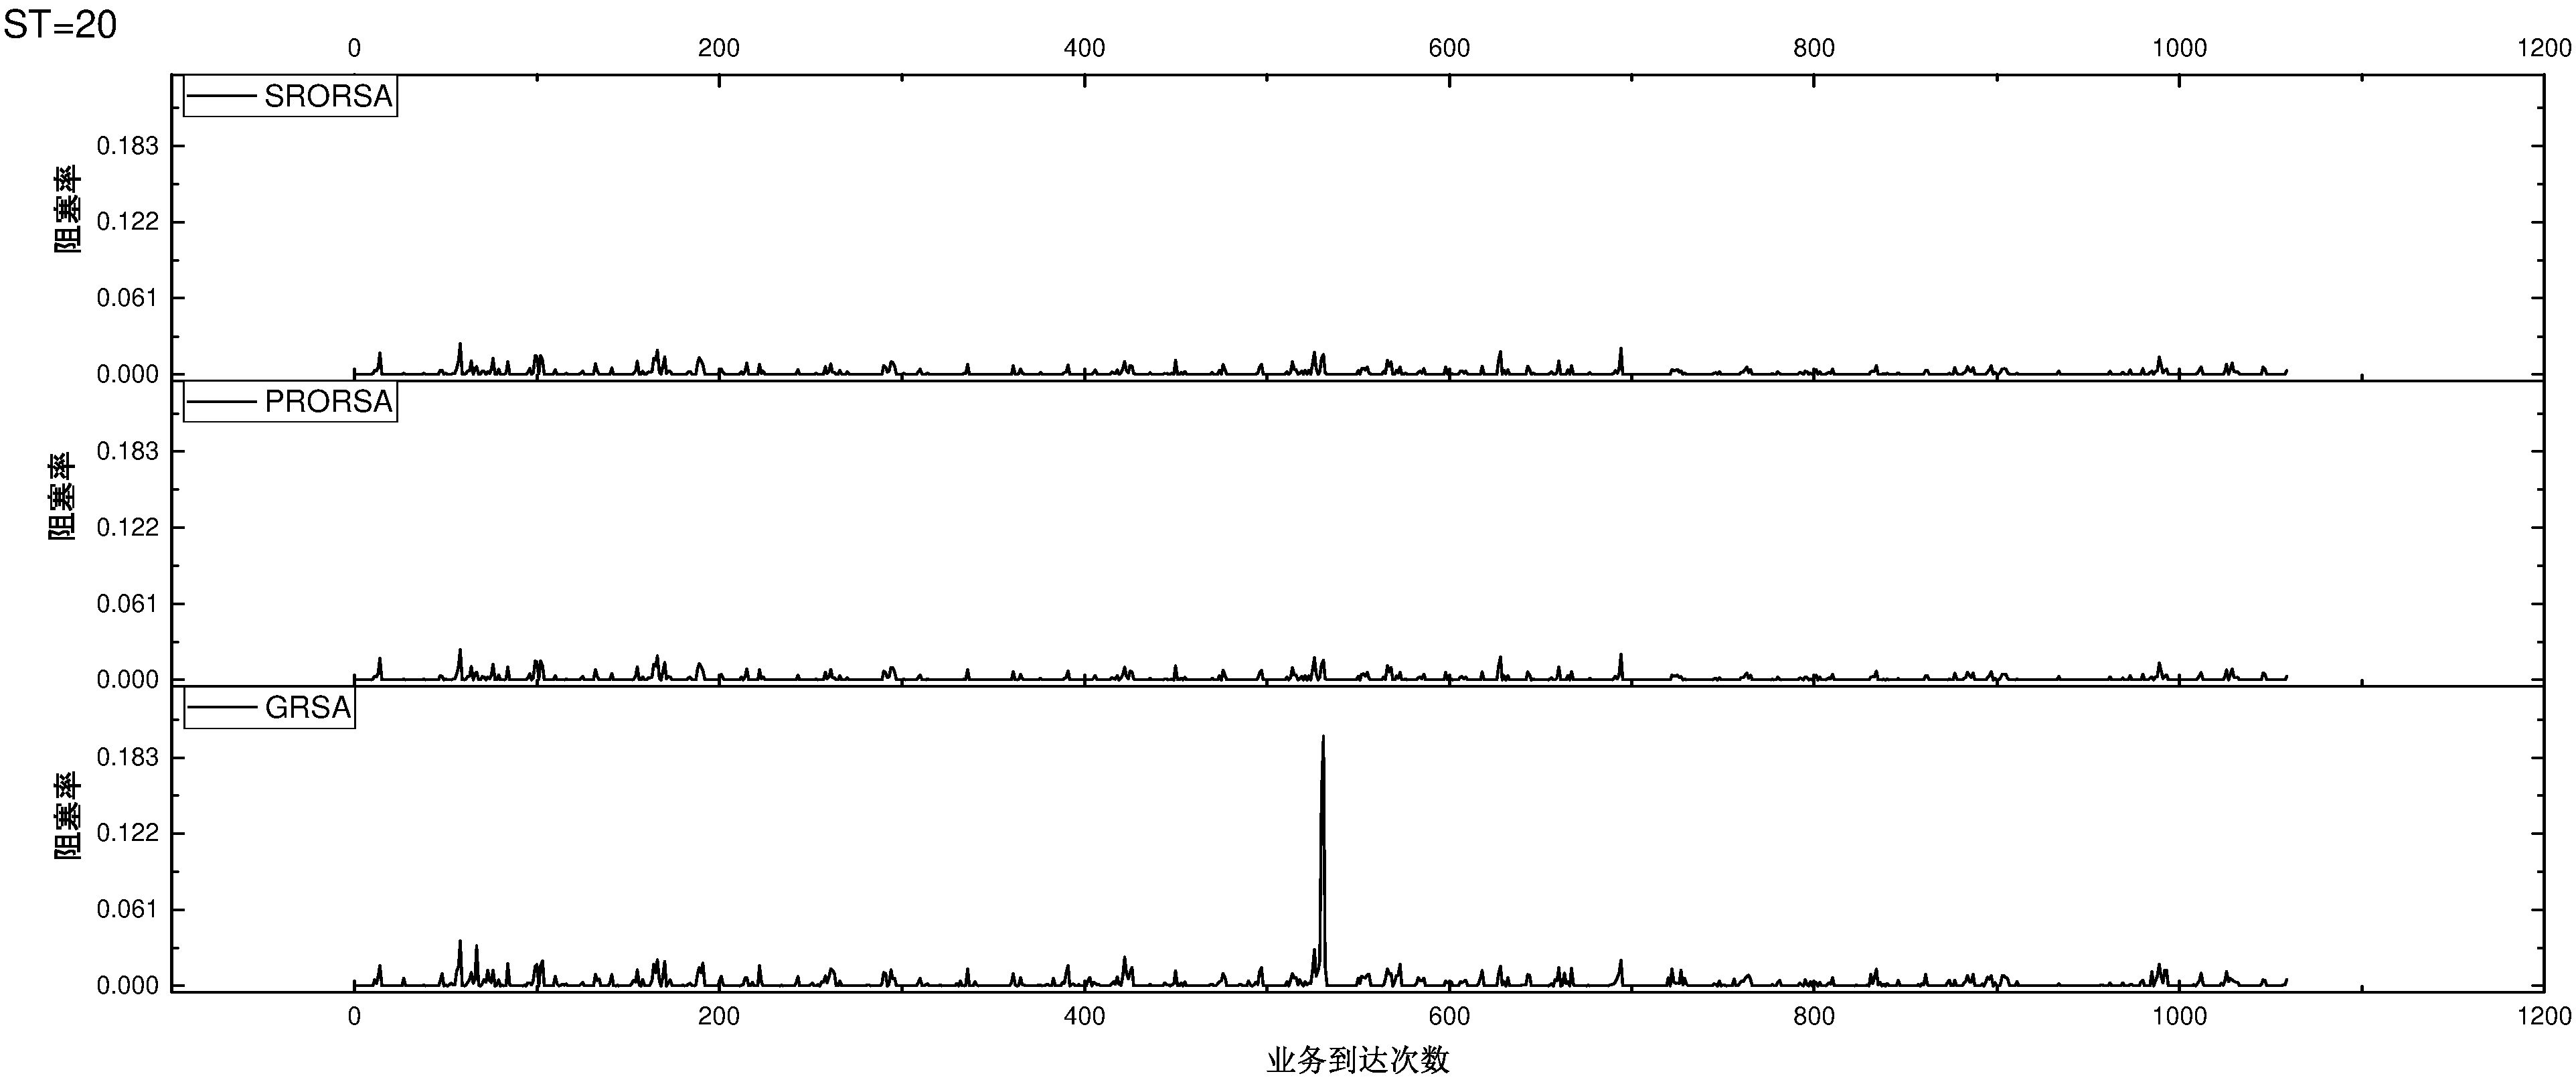
\includegraphics[width=1 \textwidth]{figures/H20Z.pdf}}
\end{center}
\caption{{\footnotesize{带权图阻塞率对比(ST=20)}}}
\label{H20Z}
\end{figure*}
\begin{figure*}
\setlength{\belowcaptionskip}{-0.5cm}
\begin{center}
{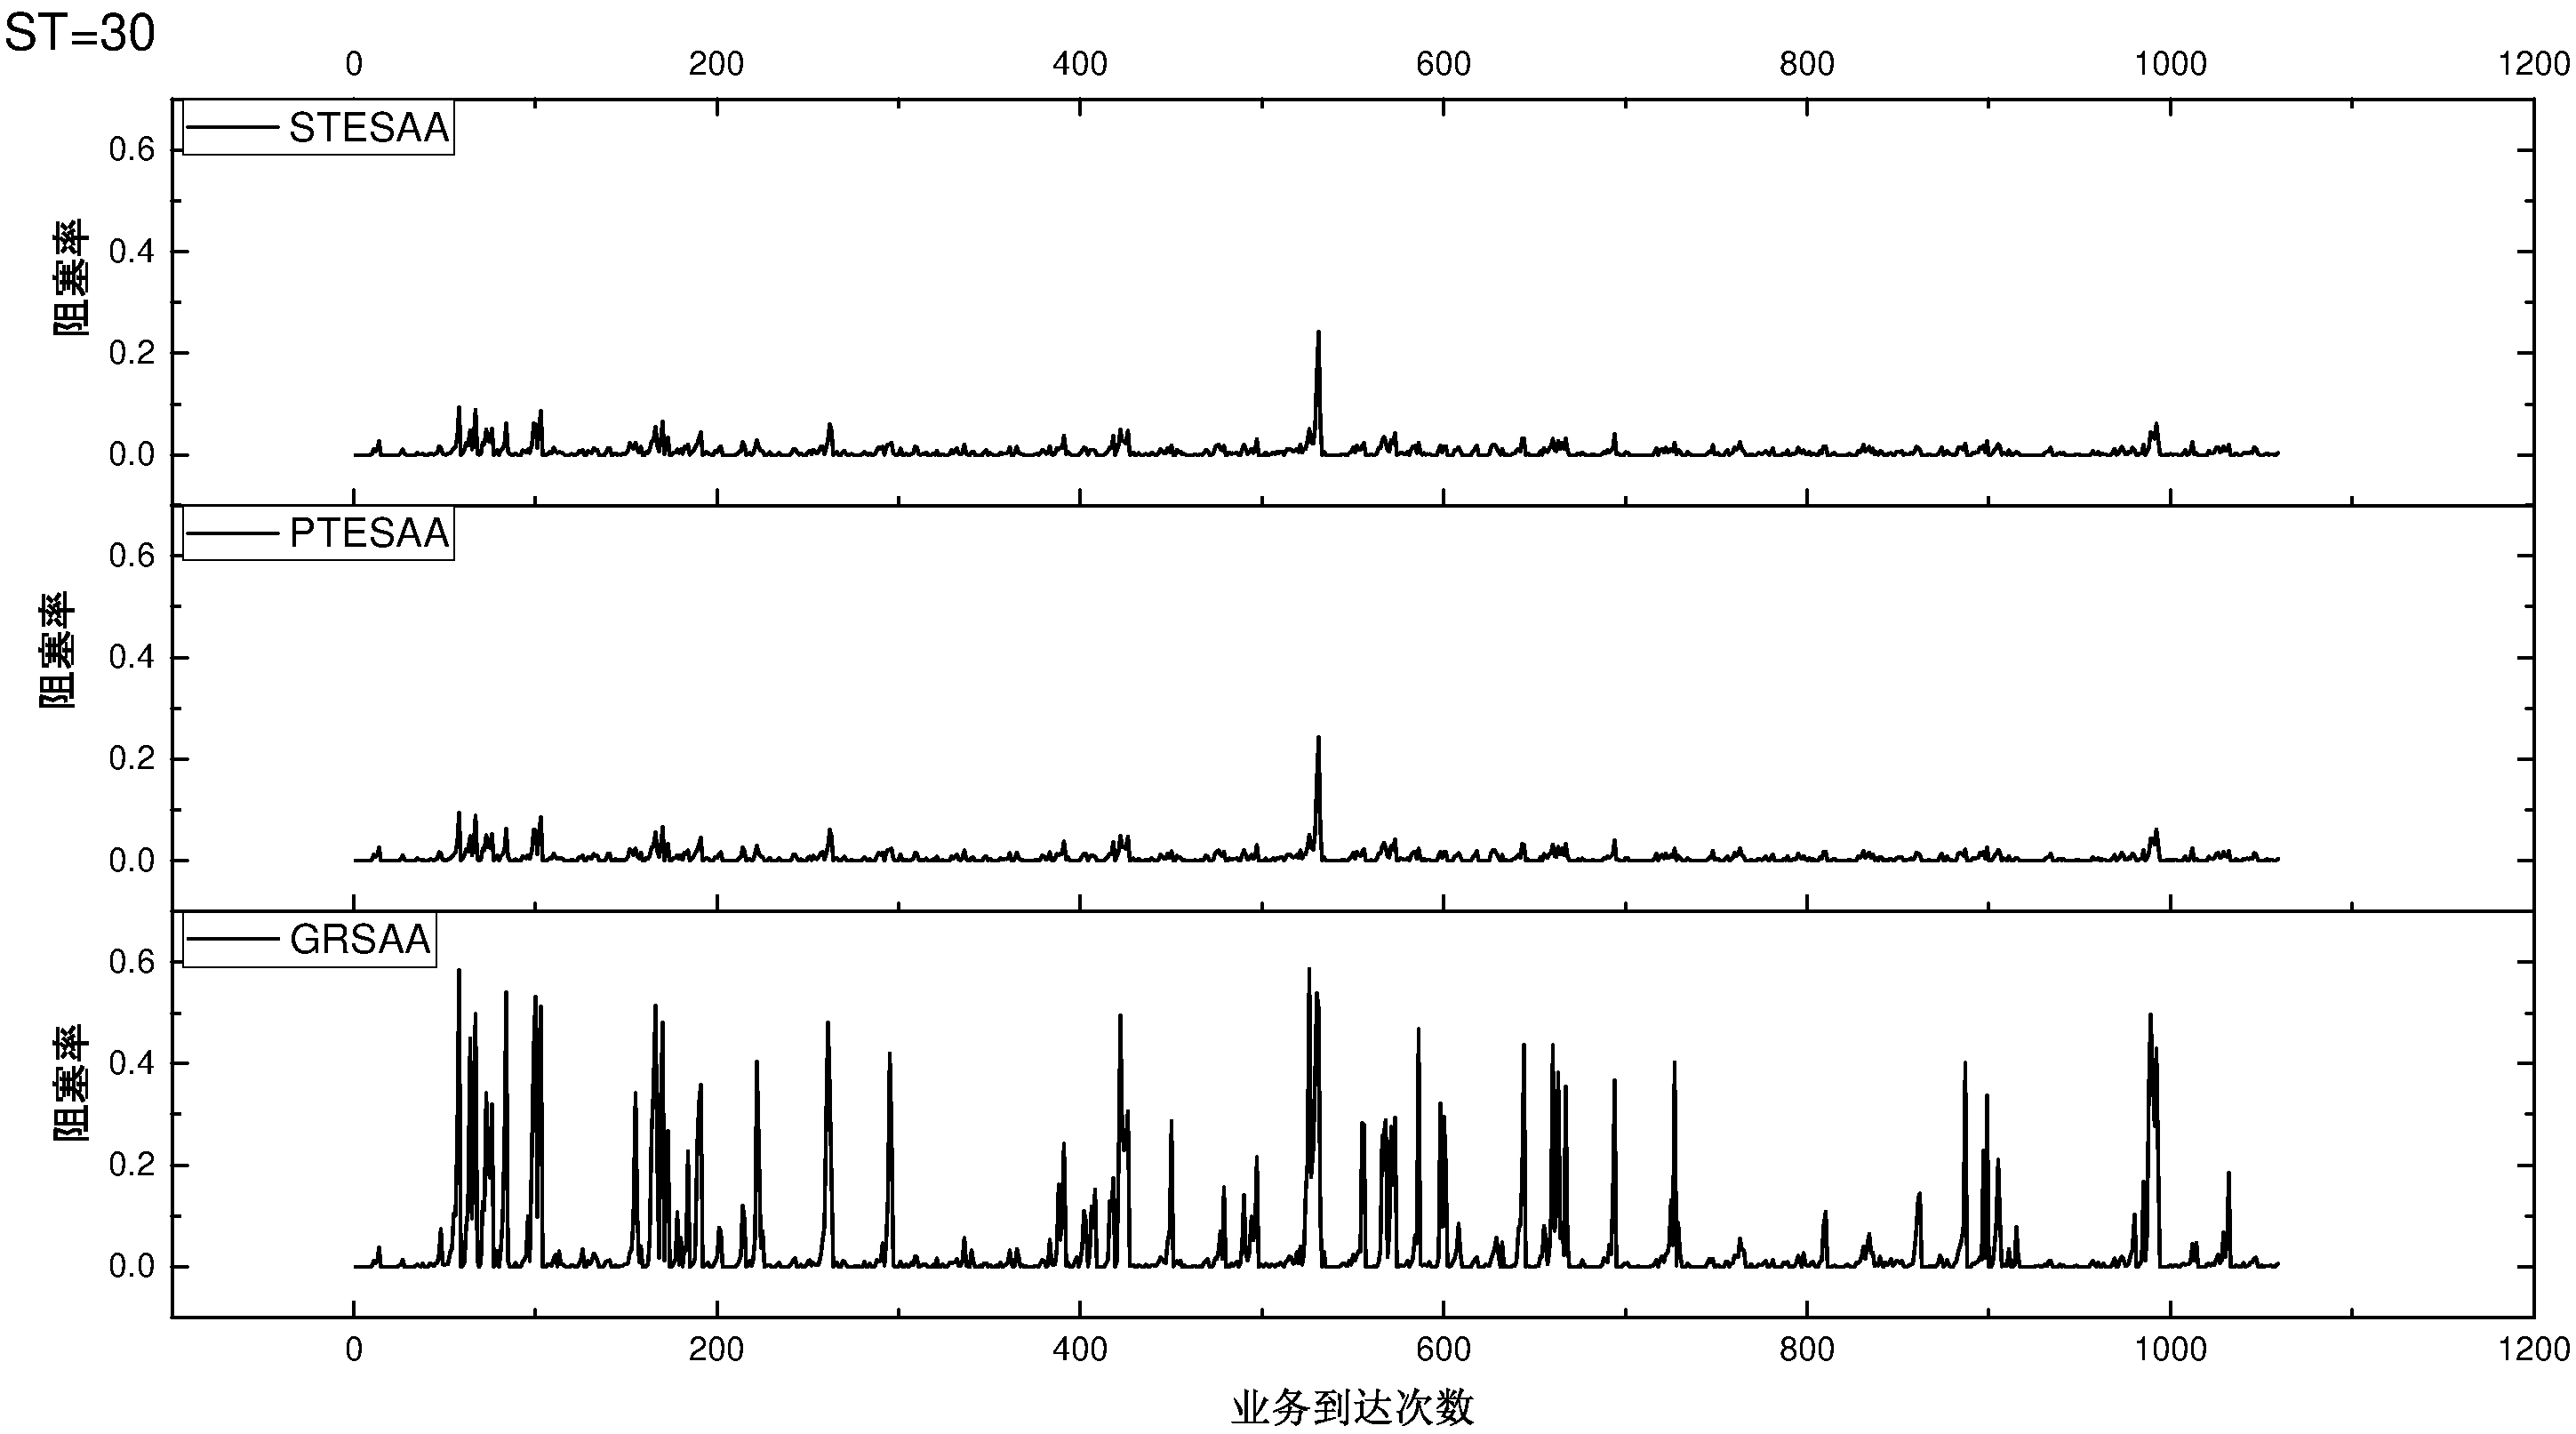
\includegraphics[width=1 \textwidth]{figures/H30Z.pdf}}
\end{center}
\caption{{\footnotesize{带权图阻塞率对比(ST=30)}}}
\label{H30Z}
\end{figure*}
\begin{figure*}
\setlength{\belowcaptionskip}{-0.5cm}
\begin{center}
{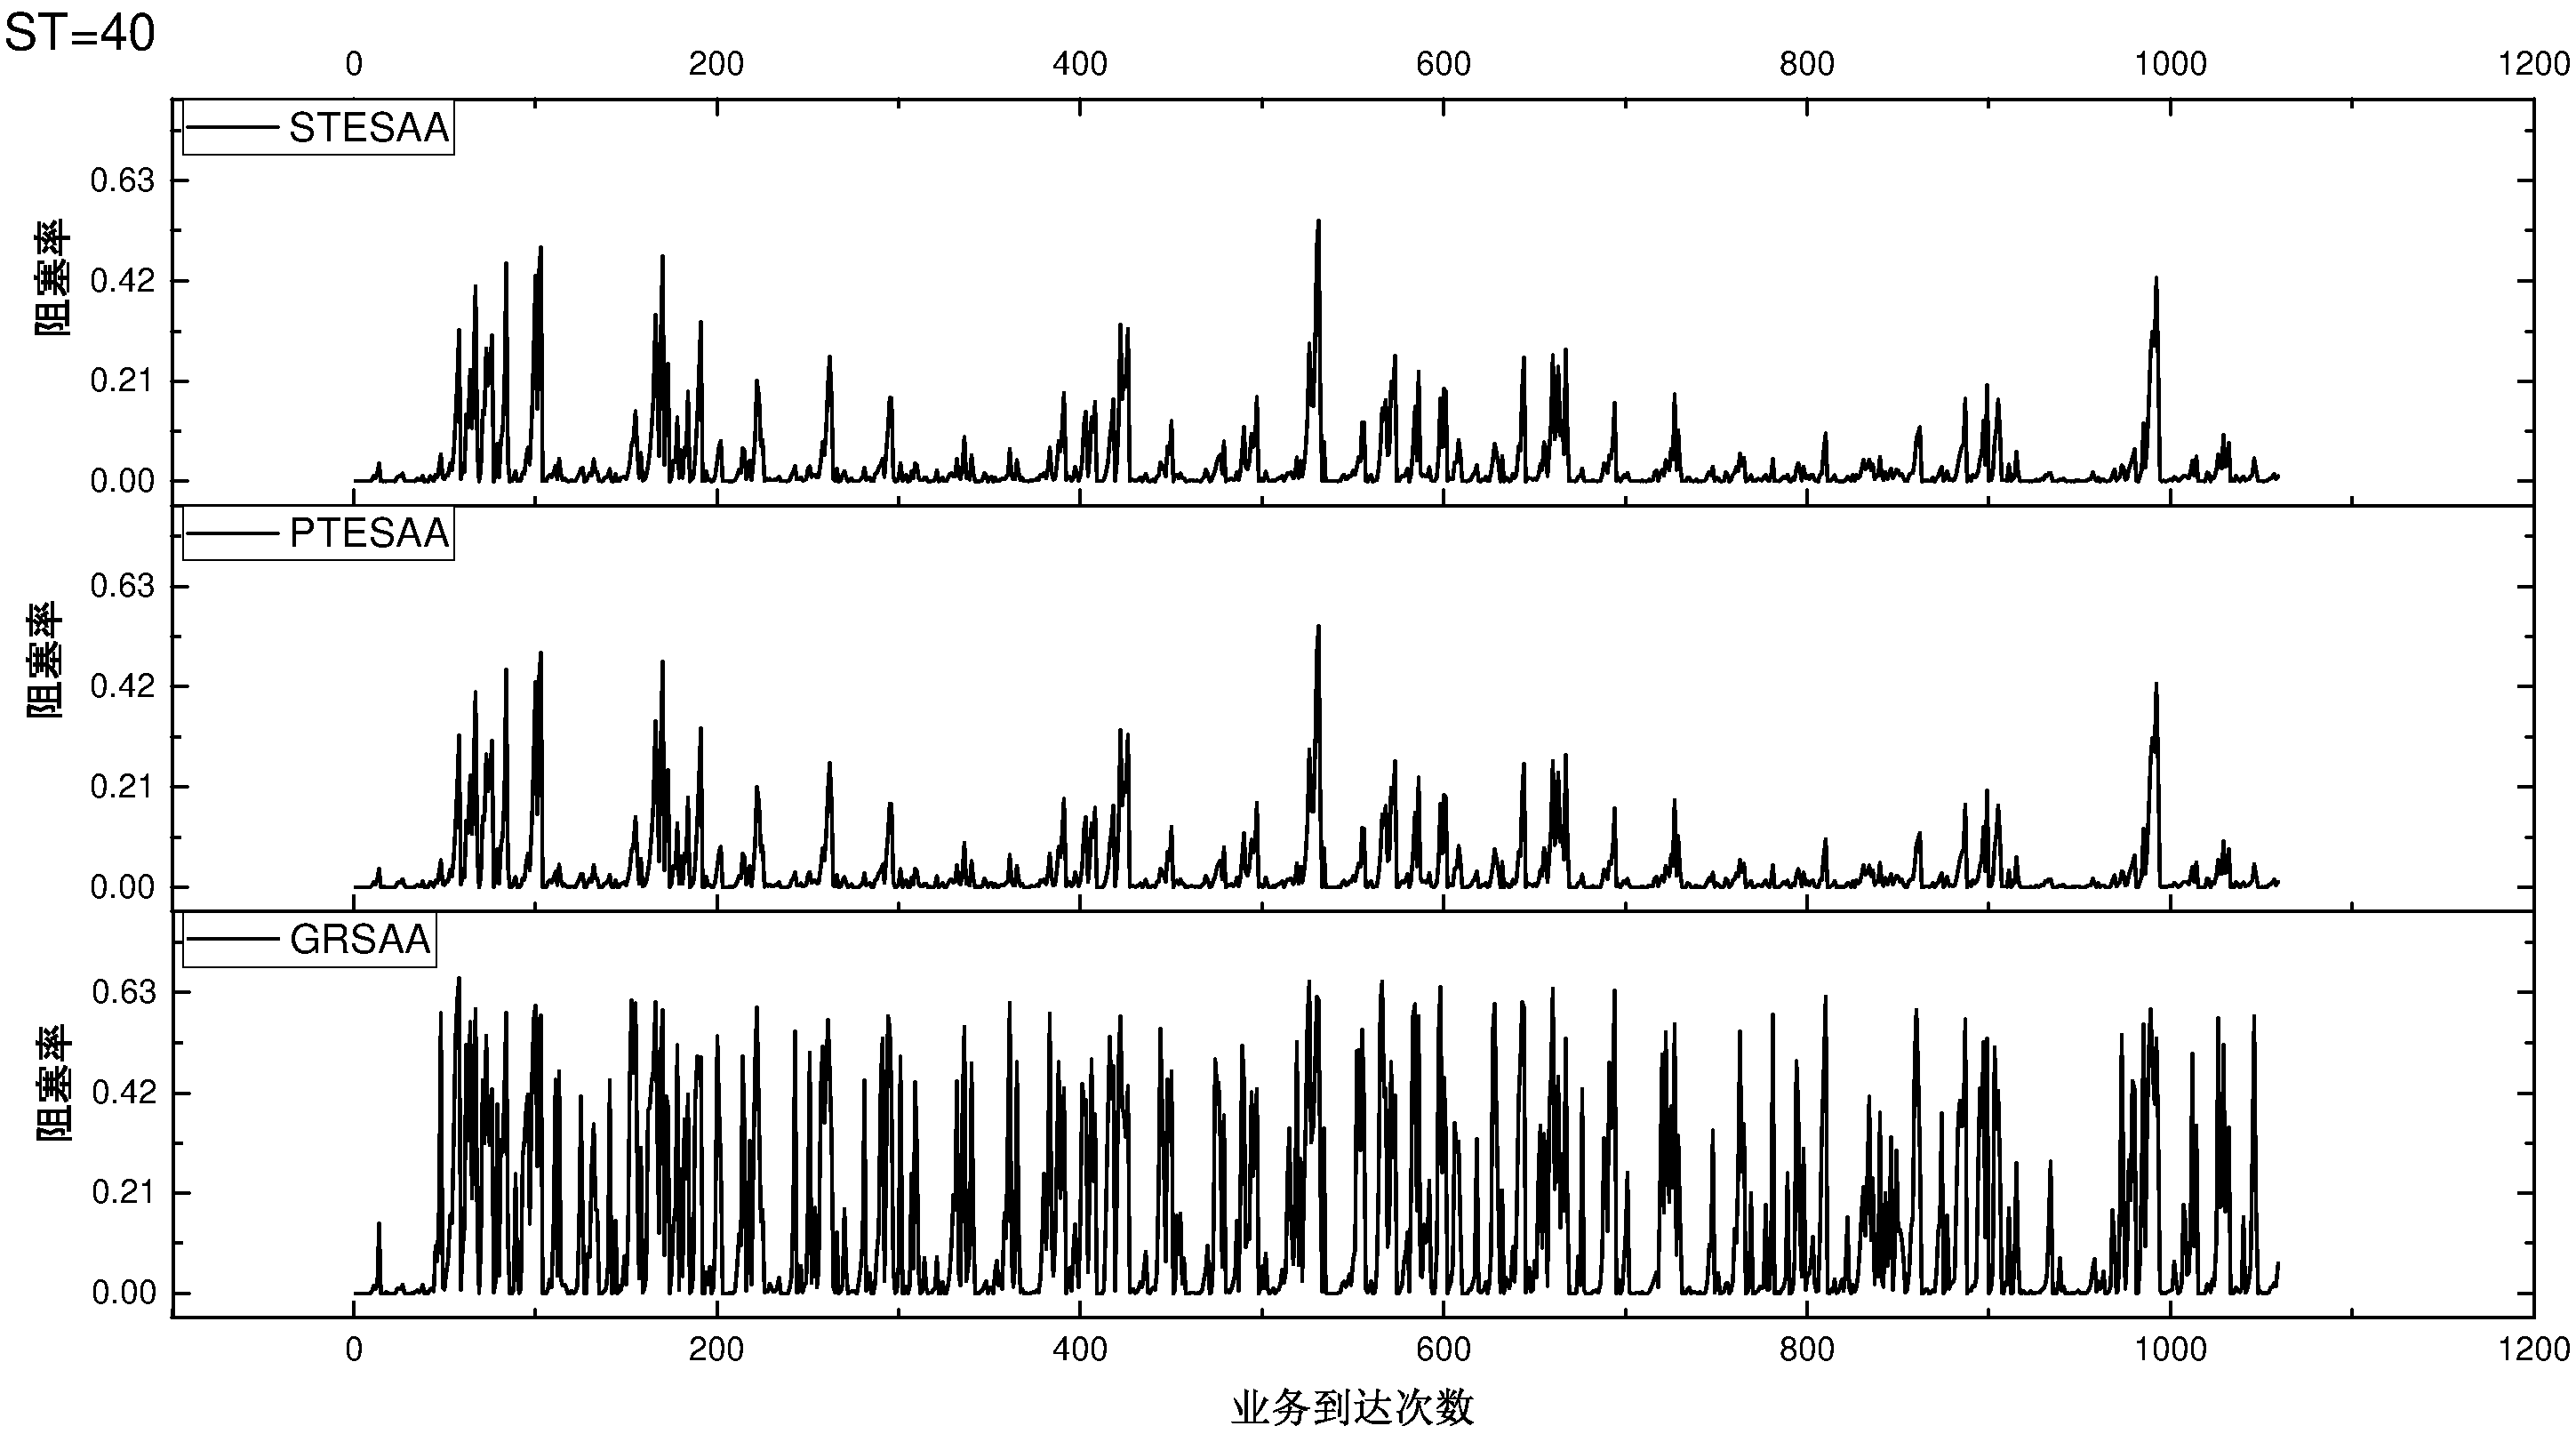
\includegraphics[width=1 \textwidth]{figures/H40Z.pdf}}
\end{center}
\caption{{\footnotesize{带权图阻塞率对比(ST=40)}}}
\label{H40Z}
\end{figure*}
\section{本章总结}
本章首先讨论了EON中的RSA问题,介绍了分层图模型,针对分层图模型设计了RORSA的算法框架,对框架中路由计算部分进行了并行设计,分别在无权图和带权图两种情况下设计了基于GPU的并行算法,实验发现RORSA能够大大优化路径跳数,路径代价和阻塞率,同时,并行算法PRORSA能加速达到5被以上。
